% =====================================================================
% MSc Thesis — Efficiently Verifying Public Key Exchange in Secure
% Messaging Protocols. Key Transparency for Signal: Dual-Index
% Warnings and Windowed Consistency Proofs
%
% Mohammad Saiful Islam — King's College London — Supervisor: Dr. B. Dowling
%
% OVERLEAF SETUP: upload this whole folder as a project; compiler:
% pdfLaTeX; main document: main.tex.
%
% HOUSE RULES (from supervisor feedback — enforce in every chapter):
%  F1  Every \section and \subsection starts with a signpost paragraph:
%      "In this section we introduce X. This is relevant because Y."
%      Never put two headers adjacent with no text between.
%  F11 Use the notation macros in kt-macros.sty EVERYWHERE (\pkid{A},
%      \sharedS, \lblself, \lblpeer, \lblwarn, ...). Never invent ad-hoc symbols inline.
%  F21 Never show an equation without defining every symbol right below
%      it on first use.
%  F17 Non-breaking space before citations: "CONIKS~\cite{melara2015coniks}".
%  RFC Every construction cites its spec: RFC 9162 (log proofs),
%      RFC 9381 (ECVRF), RFC 5869 (HKDF), draft-ietf-keytrans-protocol.
%  Recap rule: when reusing a concept introduced >2 pages back, add
%      "recall that ... (\cref{...})".
%  Writing order: Ch2 -> Ch3 -> Ch4 -> Ch5 -> Ch6 -> Ch7 -> Ch1 (last).
% =====================================================================
\documentclass[11pt,a4paper,oneside]{report}

\usepackage[utf8]{inputenc}
\usepackage[T1]{fontenc}
\usepackage[margin=2.5cm]{geometry}
\usepackage{amsmath,amssymb,amsthm}
\usepackage{mathtools}
\usepackage{booktabs}        % professional tables
\usepackage{graphicx}
\usepackage{float}           % [H] to pin figures exactly where placed
\usepackage{setspace}        % 1.5 line spacing (UK MSc convention)
\usepackage{tikz}
\usetikzlibrary{arrows.meta,positioning,calc,shapes.geometric}
\usepackage{pgfplots}        % benchmark plots (D12)
\pgfplotsset{compat=1.18}
\usepackage{xcolor}
\usepackage{microtype}
% Allow TeX a last-resort stretch so long unbreakable inline math (e.g. the VRF
% signatures in the definitions/appendix) cannot overrun the right margin.
\setlength{\emergencystretch}{4em}
\usepackage{siunitx}         % \SI{159}{\micro\second} etc.
\usepackage[ruled,vlined,linesnumbered]{algorithm2e} % Algorithms 1-3
\usepackage{tcolorbox}       % Expt security-game boxes (prof style, F25)
\tcbuselibrary{skins,breakable}
\usepackage{csquotes}
\usepackage[backend=biber,style=ieee,sorting=none]{biblatex}
\addbibresource{references.bib}
\usepackage[hidelinks]{hyperref}
\usepackage[capitalize,nameinlink]{cleveref}
\crefname{appendix}{Appendix}{Appendices}
\Crefname{appendix}{Appendix}{Appendices}
\usepackage{kt-macros}       % ALL project notation lives here

% ── Definition/theorem environments: intuition first, then formal ──
\theoremstyle{definition}
% One shared counter across all theorem-like environments, reset per chapter,
% so Definition / Lemma / Theorem / Remark number continuously (e.g. Definition
% A.13, Lemma A.14) instead of each restarting at A.1.
\newtheorem{definition}{Definition}[chapter]
\newtheorem{lemma}[definition]{Lemma}
\newtheorem{theorem}[definition]{Theorem}
\newtheorem{remark}[definition]{Remark}

% Every Definition gets an "intuition" lead-in (F23/F26):
%   \begin{definition}[Merkle log tree]\label{def:log}
%     \intuition{A tamper-evident list: one short fingerprint commits
%     to every entry, and any change to history changes the fingerprint.}
%     Formally, ...
%   \end{definition}
\newcommand{\intuition}[1]{\emph{Intuition: #1}\\[2pt]}

% ── Experiment block for security games (ACKA-paper style, F25) ──
% A proper framed box in the clean crypto-paper style (thin black rule all
% round, white background, bold title with a rule under it, then the numbered
% game lines) — NOT a shaded/rounded tcolorbox that reads as a "note". Mirrors
% the experiment layout of ACKA (Dowling & Hale, Fig. 7).
\newsavebox{\exptboxsave}
\newenvironment{exptbox}[1]{%
  \par\addvspace{\medskipamount}%
  \setlength{\fboxsep}{8pt}\setlength{\fboxrule}{0.6pt}%
  \begin{lrbox}{\exptboxsave}%
  \begin{minipage}{\dimexpr\linewidth-2\fboxsep-2\fboxrule\relax}%
  {\bfseries #1}\par\vspace{3pt}\hrule\vspace{5pt}%
}{%
  \end{minipage}%
  \end{lrbox}%
  \noindent\fbox{\usebox{\exptboxsave}}\par\addvspace{\medskipamount}%
}

\begin{document}
\onehalfspacing              % 1.5 line spacing throughout the body

% ===================== TITLE PAGE =====================
\begin{titlepage}
\centering
\vspace{0.4cm}
{\LARGE\bfseries Efficiently Verifying Public Key Exchange in Secure Messaging Protocols\par}
\vspace{0.4cm}
{\large\itshape DUET: A Key Transparency Logging Scheme with Dual-Index Warnings and Windowed Consistency Proofs\par}
\vspace{2cm}
{\large Mohammad Saiful Islam\par}
\vspace{12cm}
{\large A dissertation\\Submitted in partial fulfillment of the requirements for the degree of\par}
\vspace{1cm}
{\large MSc Advanced Computing\par}
{\scshape King's College London\\Department of Informatics\par}
\vfill
{\large August 2026\par}
\end{titlepage}

% ===================== DECLARATION =====================
\chapter*{Declaration}
I declare that this thesis, and the work presented in it, are my own. Where I have consulted or
drawn on the published and unpublished work of others, this is always clearly attributed, and where
I have quoted from the work of others, the source is always given. With the exception of such
quotations and attributions, this thesis is entirely my own work. It has not been submitted, in
whole or in part, for any other degree or qualification at this or any other institution.

The accompanying software artefact is likewise my own work, with the exception of the third-party
material identified in its \texttt{DECLARATION.md} file: the Signal Desktop client is an existing
open-source project (Signal Messenger, LLC, licensed under AGPL-3.0) into which the DUET components
were integrated, and the Rust reference implementation depends on standard, freely available
libraries.

\vspace{1cm}
\noindent Mohammad Saiful Islam\\
August 2026

% ===================== FRONT MATTER =====================
\begin{abstract}
The security of end-to-end encrypted messaging rests on an assumption its cryptography does
not itself establish: that the public keys the server hands out are authentic. Signal's
original built-in defence, the Safety Number, covers only the long-term identity keys and requires a
manual out-of-band comparison that few users ever complete, leaving a malicious or compromised
directory free to substitute a key undetected. Key transparency answers the malicious-server
problem by publishing the directory as a verifiable, append-only log, and now ships in
production --- most recently as Signal's optional Automatic Key Verification --- but deployed
designs still leave two gaps: a key substituted in the log itself is noticed only by its owner,
with no in-band channel to warn the peer, and a client returning after an offline period must
pay a monitoring cost that grows with the number of missed epochs, i.e., with the time spent
offline.

To close both gaps, we propose DUET (DUal-index, Epoch-windowed Transparency), a key
transparency scheme for secure messaging that remains aligned with the emerging IETF Key
Transparency protocol and is demonstrated through an implementation in Signal Desktop. DUET
rests on two underlying mechanisms. First, the
\emph{dual-index warning scheme} derives, from each conversation's shared secret, a pair of
participant-specific lookup labels together with a shared warning label, enabling automatic,
in-band detection of key substitution by both participants without additional user interaction.
Second, \emph{windowed consistency proofs} replace per-epoch catch-up with a single consistency
proof between the last trusted and current tree heads, making offline synchronization independent
of the duration of the offline period.

Measured on a directory of up to $10^6$ labels, the dual-index lookup proof has a median size of
\SI{817}{B} --- at parity with CONIKS, while adding automatic detection without enlarging the per-lookup proof --- and
median full client verification stays below \SI{150}{\micro\second} and is effectively independent of directory size.
Windowed catch-up sends \SI{320}{B} in place of \SI{222528}{B} at a one-month offline window, a
\num{695}-fold reduction. A two-client demonstration shows substitution and equivocation being
detected in band, with the warning surfaced in the client interface.

These results show that DUET's combination of automatic, in-band key-substitution detection and
window-independent offline consistency can be added to a messaging directory at Signal's scale
at essentially the cost it already pays, and the thesis sets out what remains between the
measured prototype and a production deployment.
\end{abstract}

\chapter*{Acknowledgements}
I am grateful to my supervisor, Dr.\ Benjamin Dowling, whose work on Authenticated Continuous
Key Agreement motivated this project and whose guidance shaped it throughout. I thank the
Department of Informatics at King's College London for its support over the course of the MSc,
and my family, whose encouragement made this work possible.

\tableofcontents
\listoffigures
\listoftables

% NOTATION TABLE — prof insists on consistent notation (F11).
% Keep this synchronized with kt-macros.sty. One row per macro.
\chapter*{Notation}
% The \small must stay scoped to this table: unbraced, it leaks into every
% chapter and appendix that follows and silently sets the whole body a size
% smaller (it cost the document ~13 pages before this was caught).
\begingroup
\small
\begin{tabular}{@{}lp{9.5cm}@{}}
\toprule
Symbol & Meaning \\
\midrule
$\A, \B$ & honest parties (Alice, Bob); $\Srv$: server; $\Adv$: adversary \\
$\pkid{U}, \skid{U}$ & long-term identity key pair of user $U$ \\
$\spk{U}, \sig{\spk{U}}$ & signed pre-key and its signature under $\skid{U}$ \\
$\opk{U}{i}$ & $i$-th one-time pre-key of $U$ \\
$\ek{U}$ & ephemeral key of $U$ \\
$\xIK{U},\xSPK{U},\xOPK{U},\xEK{U}$ & X3DH-spec notation for $\pkid{U},\spk{U},\opk{U}{i},\ek{U}$ \\
$\sharedS$ & X3DH shared secret \\
$\DH{X}{Y};\ \KDF$ & Diffie--Hellman value of two key pairs; key-derivation function \\
$\Hash$ & collision-resistant hash $\{0,1\}^*\!\to\!\{0,1\}^{256}$ (SHA-256) \\
$\ell_{\mathsf{self}}, \ell_{\mathsf{peer}}, \ell_{\mathsf{warn}}$ & dual-index labels: own-key lookup, peer-key lookup, and shared warning slot \\
$t$; $\STH_t$ & epoch number; signed tree head at epoch $t$ \\
$h_t$; $r_t$ & log-tree root; prefix-tree root at epoch $t$ \\
$\pincl, \pcons, \pvrf$ & inclusion / consistency / VRF proofs \\
$W$ & offline window (epochs); $N$: number of labels; $E$: number of epochs \\
$\concat$ & byte-string concatenation \\
\bottomrule
\end{tabular}
\endgroup

% ===================== CHAPTERS =====================
\chapter{Introduction}\label{ch:intro}

Private messaging is now part of everyday personal, professional, and civic communication.
Signal~\cite{signal-home} is a widely used end-to-end encrypted messenger. Its cryptographic design
has influenced other messaging systems~\cite{signal-protocol-impact}. The Signal Protocol, introduced
in \cref{sec:bg-signal}, provides its end-to-end encryption. Signal's practical use and the protocol's
wider influence make it an important setting for studying key authentication in asynchronous private
messaging.

For journalists, activists, abuse survivors, and others whose safety may depend on confidential
communication, encryption alone is not sufficient. A message must be encrypted under the intended
recipient's authentic key. A silent key substitution defeats that guarantee while leaving the
conversation looking secure. An attacker may then read or alter communications without giving either
user an immediate indication that the channel has been compromised. Detecting such substitution is
therefore particularly important where a loss of confidentiality could cause serious harm.

End-to-end encryption protects message content only when it is encrypted to the intended recipient's
authentic key. In asynchronous messengers such as Signal, clients obtain that key from
provider-operated infrastructure. The public-key directory is therefore a critical trust point. If the
infrastructure substitutes an attacker's key for the recipient's, the protocol may establish an
encrypted channel with the attacker. This is a key-substitution, or ``fake-key,'' attack. The
encryption layer cannot distinguish the substituted key from the intended recipient's authentic key.

The traditional defence is a manual \emph{safety-number} comparison in which the two users in a
conversation compare a displayed code over a separate, out-of-band channel. The comparison is sound
when completed, but users rarely complete it without guidance. In one study, only about 14\% of
unguided pair--application trials succeeded. Just two of twelve pairs completed the comparison in any
of the applications tested~\cite{vaziripour2017}. Even a successful comparison is a one-off check that
says nothing about later key changes.

A messaging service's public-key directory maps user identities to their public identity keys.
\emph{Key transparency} (KT) addresses this limitation by committing directory states to a verifiable,
append-only history. Clients can then check their keys against a consistent record. Signal uses KT in
its optional Automatic Key Verification feature~\cite{signal-akv}.

For a substitution committed within the directory, existing systems still rely on the account holder
monitoring their own entry. A lookup can confirm that a fetched key matches the log, but this does not
tell the communicating peer that the logged key is wrong. No automatic, in-band channel warns that
peer. A returning client that monitors every epoch also incurs a cost that grows linearly with the
number of missed epochs.

Key verification in an asynchronous messenger should therefore operate automatically, warn both
parties in band, and reject a missing or invalid proof instead of accepting the key silently. A
returning client should also be able to verify missed history without downloading one proof for every
missed epoch, while keeping proof sizes and local verification costs practical.

\section{Aim and Approach}\label{sec:intro-aims}

We propose DUET (\emph{DU}al-index, \emph{E}poch-windowed \emph{T}ransparency), which performs
key-substitution checks automatically and reports warnings in band. The checks do not require a
separate manual comparison or change the asymptotic complexity of an individual lookup proof. The
complete mechanism nevertheless performs additional label-bound lookups and writes. DUET combines the
dual-index warning scheme with windowed consistency verification and is integrated into a Signal
Desktop prototype (\cref{ch:impl}). The windowed consistency mechanism replaces one proof per missed
epoch with a single proof whose size grows logarithmically in the endpoint log sizes.

DUET does not prevent a malicious provider from denying service. Its narrower goal is to ensure that a
substituted key, an invalid or missing proof, or an inconsistent directory history causes verification
to fail rather than allowing the client to accept an attacker's key silently. \Cref{ch:threat}
formalizes this distinction between detectable interference and availability.

\section{Contributions}\label{sec:intro-contributions}

This thesis makes four principal contributions.

\paragraph{Conceptual.} The \emph{dual-index warning scheme} derives a separate lookup label for each
party and a shared warning label from the conversation's shared secret. The warning label identifies a
shared slot to which either party can write an authenticated alert. For an honestly established and
monitored conversation, a malicious server cannot predict and pre-position that slot before the label
is first used. Before the warning commits, a censored write is detected through a key mismatch
alongside a proof-verified empty slot. After the warning commits, the transition audit detects any
removal as an invalid directory transition. The resulting signal allows both parties to detect the
substitution automatically and in band (\cref{sec:design-dual}).

The thesis also implements the abstract append-only-log component of the Authenticated Continuous Key
Agreement (ACKA) framework~\cite{dowling2023acka} as the DUET directory and evaluates its proof sizes
and local cryptographic costs. Within this directory, the dual-index scheme makes key substitution by
a semi-trusted operator detectable. The ACKA framework is introduced in \cref{sec:bg-acka}.

\paragraph{Cryptographic.} The cryptographic contribution applies an RFC~9162~\cite{rfc9162}
distant-head consistency proof to offline monitoring. A returning client re-verifies the log with one
proof instead of retrieving one proof for every missed epoch. The proof size stays logarithmic in the
endpoint log sizes rather than linear in the number of epochs missed (\cref{sec:design-windowed},
\cref{lem:windowed-size}). A same-head consistency lemma (\cref{lem:dualindex-consistency}) establishes
that Alice's peer lookup and Bob's self-check cannot authenticate different values under one signed
head. \Cref{ch:design} establishes these properties, and \cref{ch:eval} evaluates their costs.

\paragraph{Systems.} The systems contribution includes a standalone Rust reference implementation
comprising the \texttt{duet} crate, an HTTP directory server, and a cross-vantage auditor. It also
includes a TypeScript verifier integrated into a fork of the Signal Desktop client (\cref{ch:impl}).
The shared protocol operations in the two implementations are checked for byte-for-byte agreement
using cross-language test vectors.

\paragraph{Empirical.} The benchmark evaluation, covering metrics M1--M17, yields four principal
findings. The implemented VRF-indexed lookup proof is at rough size parity with CONIKS. The detection
channel uses additional lookups of the same shape rather than enlarging that proof. Median full-client
verification remains below \SI{150}{\micro\second} through $10^7$ labels and grows far more slowly than
$N$. A month-long offline catch-up uses a few hundred raw path-hash bytes, compared with hundreds of
kilobytes under the per-epoch baseline. The STRIDE and MITRE ATT\&CK evaluation distinguishes the
attacks detected by the implemented controls from the residual risks that remain (\cref{ch:eval}).

\section{Thesis Roadmap}\label{sec:intro-roadmap}

\Cref{ch:background} surveys the Signal stack, transparency logs, verifiable key directories, and the
ACKA framework, and derives the requirements addressed by DUET. \Cref{ch:threat} defines the threat
model and security requirements. \Cref{ch:design} presents the design and instantiates ACKA.
\Cref{ch:impl} describes the two-layer implementation and its Signal Desktop integration.
\Cref{ch:eval} evaluates the system empirically and against the threat model.
\Cref{ch:discussion,ch:lsepi,ch:conclusion} cover the discussion and future work, the legal, social,
ethical, and professional dimensions, and the conclusion. The appendices contain the formal
definitions, algorithms, implementation and test references, benchmark tables, security analyses,
traceability material, and glossary.

\chapter{Background}\label{ch:background}

This chapter establishes the background needed to understand the design of DUET. It begins with
Signal's asynchronous key-distribution model and then examines key-transparency systems and
continuous-authentication research to derive the requirements carried into \cref{ch:design}.
\Cref{app:extended-background} provides further detail on protocol mechanics, usability evidence, and
the systems reviewed in this chapter.

% ============================================================================
\section{The Signal Protocol Stack}\label{sec:bg-signal}

Signal is a widely used end-to-end encrypted messenger~\cite{signal-home,dowling2020nocompromise}. Its
protocol combines X3DH for asynchronous session establishment with the Double Ratchet for ongoing key
evolution~\cite{x3dh,doubleratchet}. The messaging server supplies the public pre-key material needed to start a
conversation while the recipient is offline~\cite{signaldocs}, so confidentiality depends on the
authenticity of keys obtained from provider-operated infrastructure.

\subsection{Key Material, Safety Numbers, and What They Cover}\label{ssec:bg-keymat}

Signal publishes a long-term identity key, a signed pre-key, and optional one-time pre-keys. The Safety
Number authenticates the parties' identity keys and account identifiers through an out-of-band
comparison~\cite{safetynumbers}. A signed pre-key is authenticated indirectly by its identity-key
signature, while one-time pre-keys are unsigned. The ceremony therefore authenticates the long-term
identity binding rather than every public value used in one session. \Cref{sec:ext-signal} provides the
full key-material notation and coverage.

\subsection{The Extended Triple Diffie--Hellman (X3DH) Protocol}\label{ssec:bg-x3dh}

X3DH lets Alice establish a shared secret $\sharedS$ with an offline Bob by combining identity,
ephemeral, signed-pre-key, and optional one-time-pre-key Diffie--Hellman terms~\cite[Section~2.4]{x3dh}.
The resulting secret initializes the later protocol stages and is also the input from which DUET
derives conversation labels. Alice verifies Bob's signed pre-key under the supplied identity key and
aborts if that signature fails~\cite[Section~3.3]{x3dh}.

When Bob's genuine one-time pre-key is absent or withheld, an attacker that substitutes Bob's identity
key and a signed pre-key valid under that identity can derive the resulting secret and impersonate
Bob. Replacing only the signed pre-key fails the signature check, while replacing only the one-time
pre-key normally causes the parties to derive different secrets. DUET targets the coordinated
substitution, whose full derivation and message sequence are in \cref{sec:ext-signal}.

\subsection{The Double Ratchet Protocol}\label{ssec:bg-ratchet}

The Double Ratchet evolves the X3DH or PQXDH secret into per-message keys, providing forward secrecy
and post-compromise recovery after the adversary becomes passive~\cite{doubleratchet,pqxdh}. It does
not re-authenticate the public keys used to establish the session, so its guarantees still depend on
an authentic initial binding. \Cref{sec:ext-ratchet} explains the key-schedule details.

\subsection{Safety Numbers and the Verification Gap}\label{ssec:bg-gap}

Signal provides manual Safety Number comparison and optional Automatic Key Verification. AKV checks a
peer's stored binding against Signal's transparency service, but its documented availability is
limited for some username and phone-number-discovery cases, and it does not provide a channel through
which a detecting client can warn the peer~\cite{signal-akv}.

Usability evidence also limits reliance on manual verification. Across unguided trials in one study,
only 14\% of pair--application trials succeeded, and only two of twelve pairs completed the ceremony
in any tested application~\cite[p.~30]{vaziripour2017}. Instructions improved
success~\cite[p.~29]{vaziripour2017}, but users still needed substantial
time~\cite[p.~36]{vaziripour2017}. ACKA and its predecessor MoDUSA authenticate evolving protocol
state, yet both retain a user-initiated comparison or an assumed secure
log~\cite{dowling2021meta,dowling2023acka}. The supporting measurements are reported in
\cref{sec:ext-usability}.

Three requirements follow. Authentication should detect coordinated substitution of
session-establishment keys, detection should not depend on a rarely completed ceremony, and a detected
substitution should reach the peer rather than remain local to the key owner.

% ============================================================================
\section{Secure Transparency Logs}\label{sec:bg-logs}

Key transparency makes the directory accountable by binding each response to a committed state. An
operator that substitutes a key must place it in a state whose later evolution can be monitored.

\subsection{Commitments and Merkle Log Trees}\label{ssec:bg-merkle}

A Merkle root commits to every leaf under a collision-resistant hash. An inclusion proof shows that a
record belongs to the committed tree, while a consistency proof shows that a later log is an
append-only extension of an earlier one~\cite{rfc6962,rfc9162}. Both proofs are logarithmic in the
relevant tree size, and they answer different questions, because inclusion authenticates one record
whereas consistency shows that committed history was not rewritten. The construction, domain
separation, and proof walkthrough are explained in \cref{sec:ext-merkle}.

Although each proof is compact, requesting one proof for every missed epoch makes a returning
client's total work grow with its offline period. DUET's windowed proof addresses this cost.

\subsection{Key Transparency Requirements}\label{ssec:bg-ct2kt}

Key transparency applies verifiable commitments to identity-to-key bindings~\cite{chase2016overlays,melara2015coniks}.
A verifiable random function maps an identity to a deterministic but outsider-unpredictable label and
proves that the mapping was evaluated correctly~\cite{rfc9381}. This resists outsider enumeration, but
it does not hide queries from the operator or conceal the directory's scale.

Local proof verification also does not establish that every observer received the same state. A malicious
operator can present Alice and Bob with different internally consistent histories, and exposing such a fork
requires signed commitments obtained from independent vantage points to be compared. DUET therefore
separates local lookup verification from cross-vantage equivocation detection. The split-view problem
and the comparison mechanisms used by existing systems are discussed further in
\cref{sec:ext-splitview}.

\subsection{The IETF KeyTrans Architecture}\label{ssec:bg-keytrans}

The IETF Key Transparency architecture combines a VRF-indexed prefix tree with a log of committed
directory states and defines search, monitoring, and auditing roles~\cite{ietf-keytrans-architecture,ietf-keytrans-protocol}.
Signal's service implements the emerging protocol with modifications~\cite{signal-kt-server}. The draft
calls for reasonable monitoring windows but does not prescribe their construction. DUET uses the same
combined-tree model and supplies a windowed consistency mechanism.

% ============================================================================
\section{Verifiable Key Directories for Key Transparency}\label{sec:bg-vkd}

A verifiable key directory is an authenticated key--value map whose membership and non-membership
answers can be checked against a public commitment. SEEMless formalized completeness, soundness, and
simulation-based privacy for this abstraction~\cite{chase2019seemless}, and later constructions refine
its update history, storage, monitoring, and privacy properties.

\subsection{Cryptographic Building Blocks}\label{ssec:bg-vkd-blocks}

Most systems combine VRF-derived labels with a sparse or path-compressed Merkle directory, and some add
a zero-knowledge set to hide information beyond the queried binding. SEEMless uses an append-only ZKS,
Parakeet an ordered ZKS, and ELEKTRA a rotatable ZKS~\cite{chase2019seemless,malvai2023parakeet,chen2022rzks,len2023elektra}.
Merkle\textsuperscript{2} instead composes a chronological log with per-key
histories~\cite[pp.~1--2]{hu2021merkle2}. \Cref{sec:ext-vkd-blocks} explains the structural
differences and terminology.

\subsection{Academic and Deployed Systems}\label{ssec:bg-vkd-academic}

The literature develops a sequence of trade-offs. CONIKS introduced VRF-indexed bindings and
epoch-by-epoch monitoring~\cite{melara2015coniks}. SEEMless formalized the directory abstraction,
Parakeet added storage compaction and witnesses, ELEKTRA addressed multi-device histories and privacy
recovery, OPTIKS reduced history cost, and PRISM moved towards whole-directory verification~\cite{chase2019seemless,malvai2023parakeet,len2023elektra,optiks2024,pusch2025prism}.
Detection in each still depends on a user, an auditor, a witness set, or a global verifier rather than
a conversation-specific warning delivered to the peer.

Two results sharpen that comparison. ELEKTRA's unsuppressible warning is raised after a full account
reset rather than after substitution of one key~\cite[p.~2]{len2023elektra}. PRISM frames the wider
problem as reliance on someone else to check, whether a user, gossiping clients, a blockchain, or an
auditor~\cite[p.~6]{pusch2025prism}. Its whole-directory proof changes who verifies the state but does
not itself provide conversation-specific peer notification.

CONIKS is the principal baseline for this thesis because it combines private VRF-derived labels with
signed epoch roots and self-monitoring. A client verifies its own binding and later exposes a fork by
comparing signed roots with another observer. Its limitations are also central here, because
monitoring work grows with the offline period, direct client gossip was left as future work, and
detection does not itself notify the communication peer~\cite{melara2015coniks}. SEEMless reduces
history cost through versioned labels, Parakeet replaces external gossip with a witness quorum, and
ELEKTRA adds signed device-key histories. Each improvement introduces a different monitoring, trust, or
deployment condition rather than removing the peer-warning gap.

Production systems demonstrate that these constructions can operate at messaging scale. WhatsApp,
Signal, Proton, Google, and Apple use different combinations of monitoring, auditing, and commitment
comparison~\cite{whatsapp2023whitepaper,signal-kt-server,goebel2023proton,google-kt,apple-ckv}, and an
independent review of the Meta implementation reports no break of its transparency
guarantees~\cite{nccgroup2023akd}. None of the cited deployments provides the peer-warning channel
defined in this thesis. The per-system mechanisms, limitations, and citations are examined further in
\cref{sec:ext-vkd-survey} and summarized in \cref{tab:bg-compare}.

The deployments also expose relevant engineering choices. WhatsApp demonstrates a public audit path at
messaging scale but disables client history monitoring in the cited configuration~\cite{whatsapp2023whitepaper}, Signal follows the
IETF architecture and uses fixed-length prefix copaths~\cite{signal-kt-server}, and Proton combines owner and
external auditing with Certificate Transparency. Proton also identifies communication of verification
failures to users as unresolved~\cite[p.~88]{goebel2023proton}. These systems establish deployment feasibility, but
their detection remains local to the account owner or an external verifier.

% ============================================================================
\section{The ACKA (Authenticated Continuous Key Agreement) Framework}\label{sec:bg-acka}

ACKA composes continuous key agreement, Continuous Entity Authentication (CEA), and an abstract secure
log~\cite[p.~18]{dowling2023acka}. CEA derives a label and a fingerprint from chained secret state and
the new public key-share at each epoch~\cite[pp.~13--14]{dowling2023acka}, and its security notion is
$\CEAsec$~\cite[p.~18]{dowling2023acka}. A forged share either collides at the honest label, producing
two fingerprints at one label, or appears under a label the impersonated party never derives and is
caught on lookup~\cite[pp.~7--8]{dowling2023acka}. The secure-log scheme $\Log$, required to satisfy
$\Logsec$, stores and returns those fingerprints~\cite[pp.~10--11]{dowling2023acka}.
\Cref{fig:bg-acka} summarizes the composition.

\begin{figure}[H]
\centering
% fig-bg-acka.tex — extracted from ch2-background.tex
% Label: \label{fig:bg-acka}
\begin{tikzpicture}[>=Stealth, font=\small,
   box/.style={draw, rounded corners, minimum width=26mm, minimum height=20mm,
               align=center, text width=24mm, inner sep=2pt},
   open/.style={draw, densely dashed, rounded corners, minimum width=26mm,
                minimum height=20mm, align=center, text width=24mm, inner sep=2pt}]
  \node[box]  (cka) at (0,0)    {\textbf{CKA}\\[2pt]\footnotesize continuous key agreement (the ratchet)};
  \node[box]  (cea) at (5.6,0)  {\textbf{CEA}\\[2pt]\footnotesize per-epoch label \& fingerprint (security: CEAsec)};
  \node[open] (log) at (11.2,0) {\textbf{LOG}\\[2pt]\footnotesize append-only, immutable log (security: Logsec)};
  \draw[->] (cka) -- node[above,font=\scriptsize]{public $T_t$}
                     node[below,font=\scriptsize]{secret $I_t$} (cea);
  \draw[->] ([yshift=2.5mm]cea.east) -- node[above,font=\scriptsize]{post} ([yshift=2.5mm]log.west);
  \draw[<-] ([yshift=-2.5mm]cea.east) -- node[below,font=\scriptsize]{query} ([yshift=-2.5mm]log.west);
  \node[align=center, text=black!55, font=\footnotesize] at (11.2,-1.9)
       {\emph{concrete realization left open}};
\end{tikzpicture}

\caption[ACKA composition]{ACKA composes CKA and CEA with the abstract
secure-log interface $\Log$, whose required security notion is $\Logsec$. Adapted from Dowling and
Hale~\cite{dowling2023acka}.}
\label{fig:bg-acka}
\end{figure}

ACKA addresses an active channel adversary and provides continuous authentication, but its detection
result is conditional on a log satisfying $\Logsec$ rather than on a directory that resists a
malicious operator~\cite[p.~7]{dowling2023acka}. ACKA assumes a common initial state associated with
trust on first use and verifies sequentially by epoch~\cite[p.~6]{dowling2023acka}. Only the receiver
learns of a forgery, and its consistency mechanism is not used for third-party fork detection. The
formal CKA definition, adversary model, abstract log construction, and receiver-only detection result
are examined further in \cref{sec:ext-acka}.

DUET supplies the verifiable directory behind $\Log$. It also adds conversation-derived lookup labels,
a shared peer-warning slot, windowed catch-up, and cross-vantage comparison of signed heads. ACKA and
key transparency therefore address complementary adversaries. ACKA authenticates evolving state
against an active channel attacker, while key transparency constrains a malicious directory operator.

% ============================================================================
\section{Comparative Analysis of Existing Systems}\label{sec:bg-compare}

Key-transparency systems differ in the objects they authenticate, the mechanisms they use to detect
misbehaviour, their support for offline recovery, and their consistency guarantees.
\Cref{tab:bg-compare} summarizes these differences.

\begin{table}[t]
\centering
\caption[Cross-system comparison of key-transparency directories.]{Cross-system comparison of
key-transparency directories across their authenticated objects, detection, offline recovery, and
consistency.}
\label{tab:bg-compare}
\footnotesize
\setlength{\tabcolsep}{3pt}
\renewcommand{\arraystretch}{1.0}
\begin{tabular}{@{}>{\raggedright\arraybackslash}p{2.0cm}>{\raggedright\arraybackslash}p{2.3cm}>{\raggedright\arraybackslash}p{2.5cm}>{\raggedright\arraybackslash}p{1.35cm}>{\raggedright\arraybackslash}p{2.15cm}>{\raggedright\arraybackslash}p{2.6cm}@{}}
\toprule
System & What it logs & Primary detection mechanism & In-band peer warning &
  Offline recovery & Consistency and fork resistance \\
\midrule
CONIKS~\cite{melara2015coniks} & username $\to$ key binding & self-monitoring & No & linear in the number of missed updates &
  STR gossip among auditors\newline direct client-to-client exchange left as future work \\
SEEMless~\cite{chase2019seemless} & identity key (versioned) & self-monitoring (client history checks) & No & per-update
  history & $\ge$1 honest auditor per epoch\newline commitments compared through gossip or a blockchain \\
Parakeet~\cite{malvai2023parakeet} & identity key & self-monitoring & No & bounded by the compaction interval & $2f{+}1$ signatures from $3f{+}1$
  witnesses \\
ELEKTRA \cite{len2023elektra} & multi-device keychains & self-monitoring & Warning only after account reset & per-update &
  external auditor \\
OPTIKS~\cite{optiks2024} & identity key (+ devices) & self-monitoring (single proof, common case) & No &
  verify before old periods are deleted & $\ge$1 auditor + bulletin board \\
PRISM~\cite{pusch2025prism} & account keys & whole-directory verification & No &
  constant-size proof & zk-rollup on a data-availability layer \\
WhatsApp (AKD)~\cite{whatsapp2023whitepaper} & identity key & public auditing & No & Not applicable in the cited configuration\newline self-monitoring disabled & signed root + public write-once (WORM) audit log \\
Signal KT~\cite{signal-kt-server,signal-akv} & account identifier $\to$ identity key, phone-number and username-hash mappings & self-monitoring and audit interfaces, optional user-triggered AKV & No &
  monitoring endpoint\newline offline-window policy not documented in the cited source & signed head and public audit endpoints\newline independent auditor deployment not documented in the cited source \\
Proton KT~\cite{goebel2023proton} & email address $\to$ Signed Key List (SKL) fingerprint & self-audit and external audit & No &
  self-audit within 90 days & CT logs and external auditing \\
Google KT~\cite{google-kt} & account keys & self-monitoring (experimental, archived 2024) & No & Not documented in the cited source & CONIKS map in a CT log \\
Apple CKV~\cite{apple-ckv} & account keys, device keys, and opt-in state & automatic device verification and E2E-encrypted CloudKit
  cross-check & No & Not documented in the cited source & on-device consistency + encrypted log-hash gossip + internal audit \\
\bottomrule
\end{tabular}

{\scriptsize\raggedright \emph{In-band peer warning} means a conversation-specific substitution
warning written by one party and verified by the other. SEEMless additionally assumes that a user
recalls their own update times. The in-band mechanisms in Apple CKV and PRISM carry commitments rather than peer-substitution
warnings. Merkle\textsuperscript{2} and ACKA are omitted because neither defines a complete
identity-to-key directory. ACKA instead assumes the secure-log interface described in
\cref{sec:bg-acka}.\par}
\end{table}

\FloatBarrier
\subsection{Implications for the Design}\label{ssec:bg-implications}

The comparison yields three requirements. First, detection must reach the peer. Existing systems assign
discovery to the key owner, an auditor, a witness set, or a global verifier, while the cited WhatsApp
configuration falls back to manual comparison after a failed
check~\cite[pp.~5, 10]{whatsapp2023whitepaper}. ELEKTRA warns only after a full account
reset~\cite[p.~2]{len2023elektra}. DUET
therefore needs a conversation-specific warning that remains available while either party is offline.

Second, catch-up must not require one proof per missed epoch. The IETF draft requests reasonable
monitoring windows without defining the mechanism~\cite{ietf-keytrans-protocol}. CONIKS identifies
linear offline monitoring as an open cost~\cite[p.~11]{melara2015coniks}.

Third, equivocation must be detectable outside the affected session. Locally valid proofs cannot show
whether another client received a different history, so signed heads must be compared across
independent vantage points. These requirements lead directly to the dual-index warning, windowed
consistency, and auditor mechanisms in \cref{ch:design}.

Proof construction introduces a separate bandwidth--privacy trade-off. Signal's fixed-length
\num{8192}-byte proof conceals directory occupancy~\cite{signal-kt-server}, whereas CONIKS transmits
the authentication path required for the queried entry~\cite[p.~10]{melara2015coniks}. The evaluation
places DUET's compressed proof within this design space.

\chapter{Threat Model and Problem Statement}\label{ch:threat}

This chapter defines the actors, adversaries, assumptions, security goals, and scope that govern the
guarantees evaluated in later chapters. It combines the malicious-directory model of key transparency
with ACKA's active-network model so that the design can be evaluated against both server-side and
in-transit key substitution.

% ============================================================================
\section{System Model and Actors}\label{sec:threat-system}

DUET considers asynchronous communication between Alice and Bob over
infrastructure operated by a service provider (\cref{sec:bg-signal}). Either party
may be offline while the other sends a message or updates key material. The system
model comprises four actors: the
communicating clients, the messaging infrastructure, the key-transparency
service, and independent auditors. Their respective responsibilities and trust
assumptions define the attack surface considered throughout the remainder of this
chapter.

The \textbf{clients}, Alice ($A$) and Bob ($B$), run the messaging application on
their own devices. They generate and hold their own secret keys, publish the
corresponding public key material, and perform all verification locally. They are
assumed honest: their devices are not under adversarial control (the boundary
where this fails is scenario X1 in \cref{sec:threat-adversary}). Clients may be
resource-constrained and intermittently connected, which is why the cost of
catching up after an offline period is a primary concern.

The \textbf{message-delivery and key-distribution server} is the provider's
infrastructure. It stores and serves the X3DH pre-key bundles that Alice needs to
start a session with Bob (\cref{ssec:bg-x3dh}) and relays ciphertext between the
parties. It is the single service-side point through which public keys reach their consumers,
and therefore the single service-side point at which a key can be substituted. The
client--service channel is the other substitution surface, modelled separately as
the network adversary (A3, \cref{sec:threat-adversary}).

The \textbf{key-transparency log server} maintains the verifiable directory and
its append-only log, answers lookup and monitoring queries with cryptographic
proofs, and publishes a signed tree head each epoch. It may be operated by the
same party as the message-delivery server. The analysis assumes the worst case
throughout: that the two are a single, possibly malicious, operator, which avoids
relying on any assumption that they do not collude.

The \textbf{auditors} are independent parties that observe the log from a second
vantage point, cross-check the tree heads the server publishes, and replay each
epoch's declared update set against the committed directory root (the per-epoch
transition audit of \cref{ch:design}). Their role in this model is fork detection
(scenario A4) and binding a malicious operator to declare every cross-epoch
mutation. The dual-index warning itself depends on neither, a separation made
precise in \cref{sec:threat-assumptions}.

The interactions between these actors define three trust boundaries
(\cref{fig:threat-arch}). The
\emph{client--server} boundary is semi-trusted: the standard key-transparency
trust configuration inherited from CONIKS and the IETF architecture (\cref{sec:bg-logs}), in
which the server is relied upon for availability but not for honesty, and not the
abstract, security-defined log that ACKA leaves to be implemented. The \emph{client--network} boundary is
untrusted: the full active network adversary described below is adopted, the same
adversary ACKA defends against in its continuous mode (\cref{sec:bg-acka}). The
\emph{server--auditor} boundary is independent: the auditor's value is that its
view of the log is obtained separately from the client's.

The system operates in one of two authentication modes, both developed in
\cref{ch:design} and referred to in this chapter only by name: a \emph{session
mode}, in which a per-conversation dual-index entry authenticates the keys of a
given session, and a \emph{continuous mode}, in which a per-ratchet-epoch
fingerprint authenticates the evolving Double Ratchet state
(\cref{ssec:bg-ratchet}). The threat model applies to both. Where a guarantee is
specific to one mode, this is indicated.

\begin{figure}[t]
\centering
% fig-threat-arch.tex — trust boundaries.
% The untrusted network is a band BETWEEN the honest clients and the operator;
% the operator sits wholly outside it, and the auditor is beyond the operator.
% Label: \label{fig:threat-arch}
\begin{tikzpicture}[>=Stealth,font=\small,
   actor/.style={draw,rounded corners,minimum width=2.3cm,minimum height=10mm,align=center}]
  \node[actor] (A) at (0,0.95)  {Alice\\\footnotesize(client)};
  \node[actor] (B) at (0,-0.95) {Bob\\\footnotesize(client)};
  \node[actor,fill=black!8] (S) at (6.0,0) {Service operator\\\footnotesize message delivery\\\footnotesize {}+ KT log server};
  \node[actor] (Au) at (10.6,0) {Auditor};
  % untrusted-network band: the medium between clients and operator only, not the
  % honest endpoints; operator wholly to its right.
  \fill[red!4,rounded corners] (1.55,-1.7) rectangle (3.75,1.7);
  \draw[dashed,red!70!black,rounded corners] (1.55,-1.7) rectangle (3.75,1.7);
  \node[red!70!black,font=\footnotesize,align=center] at (2.65,2.05) {untrusted network\\(Dolev--Yao)};
  % client--server links pass through the band
  \draw[->] (A.east) -- (S.west);
  \draw[->] (B.east) -- (S.west);
  \node[font=\footnotesize,align=center] at (6.0,-1.9) {service operator:\\semi-trusted};
  % independent auditor beyond the operator boundary
  \draw[<->,dashed,green!45!black] (S.east) -- node[above,font=\footnotesize]{independent} (Au.west);
\end{tikzpicture}

\caption[System model and trust boundaries.]{System model and trust boundaries. Clients reach the service operator across a
network controlled by a Dolev--Yao adversary. The operator provides message delivery
and the key-transparency log and is treated as one semi-trusted party. An independent
auditor observes the log from a separate vantage point.}
\label{fig:threat-arch}
\end{figure}

% ============================================================================
\FloatBarrier
\section{Adversary Model}\label{sec:threat-adversary}

The threat model combines two well-established adversary models, because the
system must reason about both network attacks and malicious key-directory
behaviour. For the network, the analysis adopts the Dolev--Yao
model~\cite{dolevyao1983}. For the infrastructure, it adopts the
semi-trusted-server model of the key-transparency literature. These adversaries
are modelled separately, and deployments may face either or both simultaneously.

\paragraph{The Network Attacker (Dolev--Yao).} Following Dolev and
Yao~\cite{dolevyao1983}, the network adversary has maximal control of the wire:
it can intercept, modify, inject, delete, and replay any message, and it can
impersonate any party in transit. It does not, on its own, control the server's
directory. This models the active man-in-the-middle that the Double Ratchet's
post-compromise security does not defend against once the adversary remains active
(\cref{ssec:bg-ratchet}), and that ACKA's continuous mode is designed to catch
(\cref{sec:bg-acka}).

\paragraph{The Infrastructure Attacker (Malicious Server).} The server is
semi-trusted: relied upon for availability but assumed to act maliciously when it
can do so without being caught. It may substitute the key it serves for a user,
censor writes a client attempts to make to the log, and equivocate by presenting
two internally consistent but divergent views of the directory to different
clients. This is the adversary key transparency was built to expose
(\cref{sec:bg-vkd}), and it lies outside ACKA's detection theorem, which assumes a $\Logsec$-secure log rather than constructing one against such a server.

\paragraph{What the Adversary Cannot Do.} The model grants the adversary the
capabilities above and no more. It cannot break the underlying primitives: it
cannot find collisions in SHA-256, solve the discrete-logarithm problem
underlying X25519, or forge an Ed25519 signature. It cannot forge a
verifiable-random-function proof without the server's VRF secret key, nor produce
a Merkle inclusion proof for an entry that was never committed to the log. It
cannot sustain equivocation without detection by an honest auditor holding a valid,
independent second-vantage head (\cref{sec:threat-goals}). And it cannot
compromise an honest client's device: endpoint security is out of scope, and the
boundary case where this assumption is lifted is scenario X1.

The implications of these adversary capabilities for the design are developed in
\cref{ch:design}.

\Cref{tab:threat-attacks} summarizes the attack scenarios this adversary model
admits, ranging from the honest baseline (A0) through the
attacks the system is designed to detect (A1--A5) to the boundary case it does not
address (X1). Each scenario is evaluated experimentally in \cref{ch:eval}.

\begin{table}[H]
\centering
\caption{Attack scenarios, adversaries, and detection mechanisms.}
\label{tab:threat-attacks}
\setlength{\extrarowheight}{2pt}
\small
\begin{tabularx}{\textwidth}{@{}ll>{\raggedright\arraybackslash}X>{\raggedright\arraybackslash}X@{}}
\toprule
Scenario & Adversary & Objective & Detection mechanism \\
\midrule
A0 & none & honest baseline & all checks pass \\
A1 & malicious server & substitute a user's key & self-check + peer warning \\
A2 & malicious server & substitute a key and censor the warning & substitution + missing warning \\
A3 & network (Dolev--Yao) & substitute a key in transit & divergent labels + global identity binding \\
A4 & malicious server & equivocate (split-view) & cross-vantage auditor \\
A5 & malicious server & substitute during a key rotation & identity re-fetch + predecessor cross-signature + warning \\
X1 & endpoint holder & impersonate using the victim's key & out of scope (boundary) \\
\bottomrule
\end{tabularx}
\end{table}

\FloatBarrier
\subsection{Attack Scenarios}\label{ssec:threat-scenarios}

The scenarios below turn the adversary model of \cref{tab:threat-attacks} into concrete attacks,
ordered from the primary key-substitution threat through its network and equivocation variants to the
endpoint-compromise boundary.

\paragraph{A1: Key Substitution.} A1 is the primary attack in the model. A
compromised or coerced server writes its own key in place of the victim's. The
substituted key is internally consistent: the malicious server has
legitimately appended the forged key to its own Merkle log and can produce valid
inclusion proofs for it, so the Merkle proofs alone do not detect A1. Detection instead comes from
the victim observing the wrong key under its own name and from the peer learning
of the substitution through the in-band warning channel. The evaluation
(\cref{ch:eval}) instantiates A1 in two forms: A1a, substitution of the global
identity slot, and A1b, substitution of an immutable dual-index session slot.

\paragraph{A2: Warning Censorship.} A2 concerns censorship before the warning commits. After
detecting a key mismatch, the client verifies the warning slot. A proof-verified empty slot raises the
compound A2 alarm. If a committed warning later disappears, the transition audit detects the invalid
directory transition. For a client using windowed catch-up, an in-window substitution is detected only
if the warning commits and remains present at the catch-up read (\cref{ssec:design-catchup}).

\paragraph{A3: Network Man-in-the-Middle.} With no server collusion, a
Dolev--Yao adversary substitutes a key in the bundle in transit. The two parties
then derive different shared secrets, and because the dual-index labels are
derived from that secret, they address disjoint locations in the directory: the
victim queries a label at which the impersonator never registered. In addition, the substituted
bundle diverges from the identity entry at the victim's global VRF-derived label, so the client's
comparison against that VRF-bound entry exposes the substitution independently of the missed
dual-index slot.

A3 also has a post-compromise variant that motivates the continuous mode: an
adversary that has already compromised a session and then injects a forged ratchet
key mid-conversation is invisible to a server-side audit, because the server and
log remain honest. Continuous mode detects it because each epoch logs a
fingerprint of the ratchet key, so an injected key produces a conflicting
fingerprint at the agreed label and the same warning is raised.

\paragraph{A4: Equivocation (Split-View).} Inherited from Certificate
Transparency (\cref{ssec:bg-ct2kt}), the server signs two heads at one epoch, one
for the victim and one for the auditor, and no single client can distinguish the
two views. The cross-vantage comparison of the two heads exposes the fork.

\paragraph{A5: Malicious Key Rotation.} During a legitimate key rotation,
changes to the directory are expected. A malicious server exploits this by
substituting its own key while presenting the rotation as genuine, so the peer
derives the wrong secret and lands at a different directory index. The defence
anchors a rotation to identity rather than to the session: on a rotation the peer
re-fetches the current key from the global VRF directory by user identity and compares
it against the key it already trusts, so a substituted rotation is detected as a changed
identity key rather than being accepted silently, and the dual-index warning is
the in-band backstop. The prototype's client relies on the identity re-fetch and the warning, and a
single-link cross-signature check, the new key signed by its trusted predecessor, is demonstrated in
the adversarial suite.

\paragraph{X1: Endpoint Compromise (Boundary).} Once the adversary holds the
victim's own private key, it derives the same shared secret, the same labels, and
the same proofs, and is indistinguishable from the victim. X1 marks the boundary of
key-transparency protection. Key transparency protects communication between honest
endpoints but cannot protect a compromised endpoint. The attack--defence structure of these
scenarios, separating the interposition routes that place an attacker key (A1, A3,
A5) from the concealment attempts that try to hide it (A2, A4) and from the
out-of-scope endpoint boundary (X1), is presented with the evaluation in
\cref{fig:eval-attacktree}.

% ============================================================================
\section{Justification of the Threat Model}\label{sec:threat-fair}

\paragraph{The Malicious-Server Assumption in Practice.} This is the standard
assumption of the key-transparency field. The same semi-trusted, potentially
equivocating server appears in CONIKS~\cite{melara2015coniks},
SEEMless~\cite{chase2019seemless}, Parakeet~\cite{malvai2023parakeet}, and the
IETF Key Transparency architecture, and the active network adversary is the one
ACKA~\cite{dowling2023acka} is designed to defend against. The assumption also
reflects deployment practice. Deployed end-to-end encrypted messengers commonly
rely on a key-distribution service to return users' public keys, and compromise or
coercion of that service can enable key substitution. Documented fake-key attacks
show the threat is practical rather than
hypothetical~\cite{yadav2022fakekey}. Assuming the server may misbehave is therefore a
conservative and well-precedented modelling choice.

\paragraph{Rejection of the Honest-Routing Assumption.} The model allows a network adversary to drop
messages, since no cryptographic directory can force their delivery. DUET makes such interference
observable. Censored writes, missing epochs, and invalid proofs are reported as failed checks rather
than successful verification.

One limitation remains, inherited from the trust-on-first-use assumption that also
underlies ACKA. Detection establishes that the key seen now differs from a key
trusted earlier. It cannot vouch for the first key, before any trusted baseline
exists. A substitution that predates first contact, poisoning the initial pin, is
not caught, because there is nothing to compare against. This limitation is
carried through the analysis and revisited in the discussion of limitations
(\cref{ch:discussion}).

% ============================================================================
\section{Assumptions}\label{sec:threat-assumptions}

The guarantees of the later chapters rest on the following assumptions.

The \textbf{cryptographic assumptions} are conventional: SHA-256 is
collision-resistant, so that a published commitment binds its contents
(\cref{ssec:bg-merkle}). Ed25519 is existentially unforgeable under chosen-message
attack, so that a signed tree head cannot be forged~\cite{rfc8032}, and the
verifiable random function provides both uniqueness and pseudorandomness as
specified in RFC~9381~\cite{rfc9381}, so that directory labels are deterministic
for the operator yet unpredictable to outsiders. The append-only consistency
property guaranteed by RFC~9162 consistency proofs~\cite{rfc9162} ensures that a
verified log cannot be silently rewritten between visits. These assumptions
underlie the adversary's capability limits in \cref{sec:threat-adversary}.

The \textbf{endpoint assumption} is that honest clients' devices are not
compromised. This is the X1 boundary, and lifting it places the situation outside
the scope of any key-transparency guarantee.

The \textbf{auditor assumption} is that at least one honest auditor observes the log. It is required
only for fork detection (A4) and the per-epoch transition audit (\cref{ch:design}), not for the
dual-index warning mechanism. Detection of server-side substitution (A1) and network
man-in-the-middle (A3) is performed by the communicating clients and depends on no auditor.

Finally, the model follows a trust-on-first-use (TOFU) approach. Peer-side detection acts only after a
key has been pinned. The resulting first-key limitation is justified in \cref{sec:threat-fair} and
revisited in \cref{ch:discussion}.

% ============================================================================
\FloatBarrier
\section{Security Goals}\label{sec:threat-goals}

The model defines four security goals, formalized in \cref{app:definitions} and specified in
\cref{ch:design}. \Cref{ch:eval} evaluates G1 and G2 experimentally. G3 rests on VRF pseudorandomness
with RFC~9381 conformance evidence, while G4 is evaluated under the second-vantage condition.

\paragraph{G1: Key-Substitution Detection.} If a server (A1, A5) or a network
adversary (A3) substitutes a key, an honest party detects it once an honest monitor completes the
required verified lookups and, where the peer's warning is needed, that warning write commits. For the established-pair attacks A1 and A5, G1 provides bidirectional detection through the in-band
warning. The victim detects the wrong key under its own name, and a peer that has pinned the
victim's key detects it on its next key-fetch. Either can raise the shared warning, so an offline
victim remains covered. First-contact substitution (A3) is instead caught by the divergence of the
secret-derived lookup label together with comparison against the global VRF-bound identity entry, not
by the warning channel. The scripted demonstration flags the change within one or two epochs
of the next check, which is a demonstration schedule rather than a protocol-wide latency bound.

\paragraph{G2: Consistency Across Offline Windows.} A client returning after an
offline period requests one distant-head consistency proof rather than one per missed epoch, and
confirms that the log it now sees is an append-only extension of the one it last verified. The
proof's size depends on the endpoint log sizes rather than on a proof count fixed directly to the
window $W$. The endpoints themselves grow as the log grows. This property ensures that intermittent connectivity does not impose a
verification burden that grows with the number of missed epochs. The residual growth is the
logarithmic dependence on the endpoint log sizes.

\paragraph{G3: Directory Privacy.} The mapping between a user's identity and its
directory slot is hidden from outsiders, via VRF-derived labels
(\cref{ssec:bg-ct2kt}). The limit of this goal is that it provides
directory privacy against third parties, not query privacy against the operator,
which necessarily learns which identity it is asked to resolve. Query privacy from
the operator is out of scope (\cref{sec:threat-scope}).

\paragraph{G4: Fork Detection.} An equivocating server (A4) that signs two
divergent heads at one epoch is detected by cross-vantage auditing when a valid, independent second-vantage head is available.
Absent one, the auditor reports \textsc{ConsistentNoVantage} rather than a fork verdict
(\cref{ch:impl}). G4 is the only
goal that depends on the auditor-honesty assumption (\cref{sec:threat-assumptions}).

\begin{table}[H]
\centering
\caption{Security goals, the attacks they address, and the mechanisms that deliver
them.}
\label{tab:threat-goals}
\setlength{\extrarowheight}{2pt}
\footnotesize
\begin{tabularx}{\textwidth}{@{}ll>{\raggedright\arraybackslash}Xl@{}}
\toprule
Goal & Attack(s) & Security mechanism & Auditor? \\
\midrule
G1 key-substitution detection & A1, A3, A5 & A1 and A5 use self-checks and the dual-index warning.\newline A3 uses divergent labels and the global VRF-bound identity entry.\newline A5 also uses identity re-fetch and predecessor cross-signature. & no \\
G2 offline-window consistency & general rewriting & windowed consistency proofs & no \\
G3 directory privacy & enumeration / recon & VRF-derived labels & no \\
G4 fork detection & A4 & cross-vantage auditor & yes ($\geq 1$ honest) \\
\bottomrule
\end{tabularx}
\end{table}

% ============================================================================
\FloatBarrier
\section{Out of Scope}\label{sec:threat-scope}

\begin{itemize}
  \item \textbf{Prevention.} A determined operator or network can always refuse
  service. The contribution is to ensure interference cannot masquerade as successful
  verification. A refusal or drop is observable as an unavailable or incomplete check,
  though its cause is not attributed.
  \item \textbf{Endpoint security.} A compromised device (X1) is outside the
  model. No directory mechanism can help once the adversary holds the victim's
  keys.
  \item \textbf{Query privacy from the operator.} The server learns which
  identities it is asked to resolve. DUET does not provide query privacy from the operator, a
  separate property from the directory privacy of Goal~G3 (\cref{sec:threat-goals}). A
  distributed-OPRF extension is noted as future work (\cref{ch:discussion}).
  \item \textbf{Group messaging.} The design is pairwise. Extending warning
  propagation to group settings such as Sender Keys or MLS is left to future work.
  \item \textbf{Multi-device keychains.} Extending the warning to the multi-device
  keychains ELEKTRA targets (\cref{sec:bg-vkd}) is out of scope. The model assumes one
  device per identity.
\end{itemize}

Each boundary is revisited, with the corresponding future-work direction, in
\cref{ch:discussion}.

\chapter{Design}\label{ch:design}

This chapter presents DUET's architecture, dual-index warning scheme, windowed consistency proof, and
instantiation of ACKA. \Cref{app:algorithms} gives the pseudocode, and \cref{ch:eval} evaluates the
associated costs.

\paragraph{Notation.} Hashing is domain-separated in the manner of RFC~6962
(\cref{ssec:bg-merkle}): $\Hash_{\mathsf{leaf}}(x) = \Hash(\mathtt{0x00} \concat x)$
and $\Hash_{\mathsf{node}}(l, r) = \Hash(\mathtt{0x01} \concat l \concat r)$, with
$\Hash$ instantiated as SHA-256 and $\concat$ denoting byte concatenation. The empty
position has the constant default hash $\Hash(\varepsilon)$. The prefix tree and the log
use these same leaf and node tags. Cross-tree confusion is not exploitable here, since
prefix roots appear only as log leaf data and log roots only in signed tree heads, but a
production deployment should apply distinct per-structure tags as defence in depth.
Identities are treated as fixed-width service identifiers, so concatenations of identity and
label material are unambiguous without explicit length prefixes.

% ============================================================================
\section{Architecture}\label{sec:design-arch}

The proposed architecture is built around three authenticated data structures arranged in layers,
where each layer authenticates the one below (\cref{fig:design-arch}). The prefix tree stores the
current directory state, the append-only log records every committed version of that state, and the
signed tree head authenticates the latest log root. This is the combined-tree design of the IETF Key
Transparency working group (\cref{ssec:bg-keytrans}). Lookups are served against the \emph{last
committed epoch}, never the live tree. Only a committed prefix root has been appended to the log and
can therefore be linked by an inclusion proof to a signed tree head.

\begin{figure}[t]
\centering
% fig-design-arch.tex — extracted from ch4-design.tex
% Label: \label{fig:design-arch}
\begin{tikzpicture}[>=Stealth,font=\small,
   layer/.style={draw,rounded corners,minimum width=6.4cm,minimum height=11mm,align=center}]
  \node[layer] (sth) at (0,4) {Signed Tree Head (STH)\\[-1pt]\footnotesize signed commitment};
  \node[layer] (log) at (0,2) {Append-only Merkle log\\[-1pt]\footnotesize history of directory states};
  \node[layer] (pt)  at (0,0) {Sparse Merkle prefix tree\\[-1pt]\footnotesize current authenticated directory};
  \draw[->] (pt) -- (log);
  \draw[->] (log) -- (sth);
  \node[draw,rounded corners,align=center,font=\footnotesize] (vrf) at (5.2,0) {VRF\\global labels};
  \draw[->,dashed] (vrf) -- (pt);
\end{tikzpicture}

\caption[The authenticated directory core.]{The authenticated directory core. The prefix tree,
Merkle log, and signed tree head form the commitment chain. The VRF derives global directory
labels.}
\label{fig:design-arch}
\end{figure}

\subsection{The Three Structures}\label{ssec:design-structures}

The three structures form a verification stack. A lookup proof is checked against the prefix root,
the prefix root's inclusion in the Merkle log, and the signed tree head that authenticates the log
root (\cref{ssec:design-verify}).

\paragraph{Prefix Tree.} The directory is a sparse binary Merkle tree that maps each
256-bit \emph{label} to a \emph{value}. For a user-identity entry, the value is an
identity public key. The label is the position of the entry in the tree, derived
rather than chosen, and it comes in two families: a \emph{global slot}, computed
server-side as a VRF over the user identifier, and the client-derived \emph{raw slots},
computed from conversation secrets: the per-conversation dual-index lookup slots and shared
warning slot (\cref{sec:design-dual}) and, in continuous mode, the per-epoch CEA slots
(\cref{ssec:design-modes}).

\paragraph{Append-Only Log.} Each committed prefix-tree root is appended to a Merkle
log (\cref{ssec:bg-merkle}) as a single leaf $\prefroot{t}$. The log therefore records
every committed directory state, and a consistency proof certifies that this
history has only ever grown. Nothing previously committed has been modified,
deleted, or reordered.

\paragraph{Signed Tree Head (STH).} Each epoch, the root of the log is signed with Ed25519
and published as the STH. This gives clients and auditors a single authenticated value
that commits to the whole directory and its history. It is the anchor against which
every lookup is ultimately checked.

\paragraph{Why a VRF?} The VRF carries G3 (Directory Privacy)
(\cref{sec:threat-goals}). The operator holds the VRF secret key and maps a user
identifier to a pseudorandom label, attaching a proof that the label was computed
correctly. A client verifies that proof against the operator's public key but cannot
itself compute or predict any other label (\cref{ssec:bg-ct2kt}). The labels are thus
deterministic for the operator yet unpredictable to outsiders, which prevents an
observer from enumerating the directory.

\subsection{Epoch Lifecycle: Update, Commit, and the Signed Tree Head}\label{ssec:design-epoch}

The directory evolves in epochs. An $\textsf{update}(\mathit{label}, \mathit{value})$
changes the value stored at one leaf of the current uncommitted prefix tree and recomputes only the
hashes on the path from that leaf to the root. The running time is therefore $O(256)$, one hash per level of the fixed 256-bit label space
and so constant in $N$, rather than $O(N)$. The number of \emph{transmitted} non-default siblings in the resulting proof is a
separate quantity, whose expected value is $\approx\lceil\lg N\rceil$.

A $\textsf{commit\_epoch}()$ then closes the epoch. It reads the current prefix-tree
root, appends it to the log as the next leaf, recomputes the log root, snapshots the
committed tree so that subsequent searches are served against a frozen state, and signs
the new head.

The contents of the signed tree head determine exactly what the signature
authenticates. The STH signs, under Ed25519, the 88-byte little-endian message
\begin{equation}\label{eq:design-sth}
  \mathit{epoch} \concat \mathit{tree\_size} \concat \mathit{root} \concat
  \mathit{timestamp} \concat \Hash(\mathit{config}),
\end{equation}
where $\Hash(\mathit{config}) = \Hash(\mathit{pk}_{\mathsf{vrf}} \concat
\mathit{pk}_{\mathsf{sth}} \concat \mathit{suite} \concat \mathit{version} \concat
\mathit{epoch\_interval} \concat \mathit{raw\_label\_policy})$, the trailing byte binding the
write-once raw-label policy so the server cannot silently relax it. Each field of \cref{eq:design-sth} is necessary for a different aspect of the verification procedure. The $\mathit{tree\_size}$ is
required by the inclusion and consistency verifiers. Signing the $\mathit{timestamp}$
means the timestamp cannot be altered without invalidating the signature. Enforcing \emph{freshness}
additionally requires a client-side maximum-age or publication-cadence policy, which the prototype
does not implement (\cref{ch:discussion}). The trailing $\Hash(\mathit{config})$ is a
CONIKS-style policy commitment (the field CONIKS calls $P$) that binds the provider's
parameters into the signature. With it, the server cannot silently swap its VRF key,
its signing key, the ciphersuite, the protocol version, or the epoch cadence, or
serve different parameters to different clients, because any client that recomputes
$\Hash(\mathit{config})$ from the parameters it expects will reject the mismatch. A
parameter substitution thus becomes a signed, monitorable act rather than a silent one: a uniform
mismatch is rejected by any client that recomputes the commitment, and serving different parameter
sets to different clients is equivocation on the configuration commitment, exposed by the same
cross-vantage comparison as A4.

\subsection{The Client Verification Chain}\label{ssec:design-verify}

A client accepts no server response without independently verifying it: every lookup is
ultimately authenticated against a signed tree head. Each verification traverses the same three-layer architecture
introduced in \cref{sec:design-arch}: first the prefix tree, then the append-only log,
and finally the signed tree head. The verification chain is the six-step pipeline of
\cref{fig:design-verify}.

\begin{figure}[t]
\centering
% fig-design-verify.tex — the client verification chain (VerifiedLookup).
% Label: \label{fig:design-verify}
\begin{tikzpicture}[>=Stealth,font=\footnotesize,
   vstep/.style={draw,rounded corners,text width=13cm,minimum height=8mm,align=left,inner sep=5pt},
   note/.style={font=\scriptsize\itshape,text=black!55,text width=13cm,align=left}]
  \node[vstep] (s1) {\textbf{1. Requested-label binding} (every path): require $\pi_{\mathrm{prefix}}.\mathit{label}$ equals the label the client queried, so a valid proof for a different label is rejected};
  \node[vstep,below=3mm of s1.south,anchor=north] (s2) {\textbf{2. VRF label binding} (VRF path only): verify the ECVRF proof and require $\beta[0{:}32]$ equals that same queried label (RFC~9381)};
  \node[vstep,below=3mm of s2.south,anchor=north] (s3) {\textbf{3. STH signature and log history}: verify the Ed25519 signature and require the returned head to match the caller-supplied verified head. Between lookups, the Signal Desktop verifier accepts a newer head only after a valid consistency check from the last trusted head};
  \node[vstep,below=3mm of s3.south,anchor=north] (s4) {\textbf{4. Value binding}: require the prefix proof binds to the returned value};
  \node[vstep,below=3mm of s4.south,anchor=north] (s5) {\textbf{5. Prefix root}: recompute the prefix-tree root from the proof (siblings $+$ 32-byte bitmap)};
  \node[vstep,below=3mm of s5.south,anchor=north] (s6) {\textbf{6. Log inclusion and latest-state binding}: check the recomputed root is a leaf under the signed log root, and that the inclusion covers the \emph{last} log leaf (inclusion of an older leaf does not establish the current directory state)};
  \foreach \a/\b in {s1/s2,s2/s3,s3/s4,s4/s5,s5/s6}{\draw[->] (\a) -- (\b);}
  \node[note,below=3mm of s6.south,anchor=north] {The warning slot is checked by a separate invocation of this same chain (\textsf{CheckWarning}), so its verified inclusion or non-inclusion is established independently.};
\end{tikzpicture}

\caption[The six-step client verification chain.]{The six-step client verification chain. Every lookup is checked locally
against a signed root.}
\label{fig:design-verify}
\end{figure}

The verification chain has three properties that the figure does not make evident. First, global
lookups require the step~2 VRF check, while client-derived raw labels omit it, and there the step~1
requested-label binding stands on its own. Second, the signed head used for verification must be
identical to the head the client independently obtained and verified, either the latest head it
fetched or, during catch-up, the new head whose append-only consistency with its last trusted head it
has just checked. The client rejects any response anchored to a different head, even one that carries
a valid signature, which prevents stale-snapshot acceptance and prevents an equivocating server from
substituting another signed view. Third, inclusion is pinned to the latest leaf, because each commit
appends the new directory root as the log's last leaf, so step~6 requires
$\mathit{leaf\_index} = \mathit{tree\_size} - 1$ at exactly the signed tree size, and a server
therefore cannot answer with a stale directory snapshot under the current signed head. Inclusion
proves membership, not \emph{currency} (RFC~9162~\cite[Section~2.1.3.2]{rfc9162}), and the currency
pin closes that gap.

The Rust and TypeScript implementations enforce the same six-check chain, and \cref{ch:eval} measures
the full chain. The ``full client verification'' benchmarked in \cref{ch:eval} is the complete
six-step chain.

% ============================================================================
\section{The Dual-Index Warning Scheme}\label{sec:design-dual}

The dual-index scheme meets the in-band peer-warning requirement of \cref{ssec:bg-implications} and so
achieves G1 (Key-Substitution Detection) against the substitution attacks A1, A3, and A5. An in-band
warning channel flags a server-side slot substitution (A1) and its continuous-mode counterpart (A5).
The secret-derived dual-index labels detect a network man-in-the-middle (A3), because an attacker with
a different shared secret derives disjoint labels, so the proof-verified lookup returns non-inclusion.
A comparison with the peer's global VRF-anchored directory entry also detects pre-emptive occupation
of the expected slot, because an attacker-controlled value cannot match the authenticated global key.

\subsection{Label Derivation}\label{ssec:design-labels}

The dual-index scheme allocates three directory slots to each conversation: two lookup
slots (one per party) and one shared warning slot (\cref{fig:design-dualindex}).
Alice and Bob derive these slot labels from the X3DH/PQXDH shared secret $\sharedS$
(\cref{ssec:bg-x3dh}) using HKDF-SHA256 as specified in RFC~5869~\cite{rfc5869}, the same
key-derivation function Signal already uses elsewhere:
\begin{equation}\label{eq:design-labels}
\begin{aligned}
  \mathit{PRK} &= \HKDFex(\text{salt} = \text{\texttt{"duet-dual-index"}},\ \sharedS)\\
  \ell_{\mathsf{self}} &= \HKDFexp\!\big(\mathit{PRK},\ \text{\texttt{"lookup"}} \concat \mathit{id}_{\mathsf{self}} \concat \mathit{id}_{\mathsf{peer}},\ 32\big)\\
  \ell_{\mathsf{peer}} &= \HKDFexp\!\big(\mathit{PRK},\ \text{\texttt{"lookup"}} \concat \mathit{id}_{\mathsf{peer}} \concat \mathit{id}_{\mathsf{self}},\ 32\big)\\
  \ell_{\mathsf{warn}} &= \HKDFexp\!\big(\mathit{PRK},\ \text{\texttt{"warning"}} \concat \min(\mathit{id}_\A, \mathit{id}_\B) \concat \max(\mathit{id}_\A, \mathit{id}_\B),\ 32\big).
\end{aligned}
\end{equation}
In \cref{eq:design-labels}, $\mathit{PRK}$ is the extracted pseudorandom key, while
$\mathit{id}_{\mathsf{self}}$ and $\mathit{id}_{\mathsf{peer}}$ identify the deriving party and its
peer. The $\min$ and $\max$ operations order the fixed-width identity encodings lexicographically.
Each output is 32 bytes, matching the prefix tree's label width. Canonical ordering is used only for
the warning label, which both parties must derive identically. Directional ordering gives each party a
separate lookup slot.

\begin{figure}[ht]
\centering
% fig-design-dualindex.tex — extracted from ch4-design.tex
% Label: \label{fig:design-dualindex}
\begin{tikzpicture}[font=\small,>=Stealth,
   slot/.style={draw,rounded corners,minimum width=2.6cm,minimum height=10mm,align=center},
   sec/.style={draw,rounded corners,fill=black!6,minimum width=1.9cm,minimum height=13mm,align=center},
   kdf/.style={draw,rounded corners,fill=black!3,align=center,minimum height=12mm},
   elbl/.style={font=\scriptsize,align=center}]
  \node[sec] (S) at (0,0) {$\sharedS$\\[-1pt]\footnotesize shared\\[-3pt]\footnotesize secret};
  \node[kdf,minimum width=2.9cm] (ext) at (3.1,0)
    {HKDF-Extract\\[1pt]{\scriptsize salt ``\texttt{duet-dual-index}''}};
  \node[draw,rounded corners,minimum width=1.0cm,minimum height=8mm] (prk) at (5.7,0) {PRK};
  \node[slot] (self) at (10.7,1.95)  {$\ell_{\mathsf{self}}$\\[-1pt]\footnotesize Alice's key};
  \node[slot] (peer) at (10.7,0)     {$\ell_{\mathsf{peer}}$\\[-1pt]\footnotesize Bob's key};
  \node[slot,fill=black!10] (warn) at (10.7,-1.95) {$\ell_{\mathsf{warn}}$\\[-1pt]\footnotesize shared tripwire};
  \draw[->] (S.east) -- (ext.west);
  \draw[->] (ext.east) -- (prk.west);
  \draw[->] (prk.east) -- node[elbl,above,pos=0.55]{\texttt{Expand}\\``lookup''$\,\|\,\mathit{id_A}\|\mathit{id_B}$} (self.west);
  \draw[->] (prk.east) -- node[elbl,above]{\texttt{Expand}\\``lookup''$\,\|\,\mathit{id_B}\|\mathit{id_A}$} (peer.west);
  \draw[->] (prk.east) -- node[elbl,below,pos=0.55]{\texttt{Expand}\\``warning''$\,\|\,\min\|\max$} (warn.west);
\end{tikzpicture}

\caption[The dual-index scheme's three derived slots.]{Two lookup slots and a shared warning slot
are derived from the conversation secret $\sharedS$. HKDF-Extract produces $\mathit{PRK}$.
Three domain-separated HKDF-Expand operations then produce $\ell_{\mathsf{self}}$,
$\ell_{\mathsf{peer}}$, and $\ell_{\mathsf{warn}}$. Alice and Bob share $\sharedS$, so they derive
the same warning label and can read either party's warning. A different secret $\sharedS'$ produces
a disjoint label set.}
\label{fig:design-dualindex}
\end{figure}
\FloatBarrier

This corrects two simplifications that appeared in early descriptions of the scheme: it
uses HKDF rather than a bare hash of $\sharedS$, and it uses three labels with canonical
ordering applied to the warning label alone. Cross-implementation test vectors verify the
byte-for-byte equivalence of the derivation across the Rust and TypeScript implementations on the
committed cross-language vectors (\cref{sec:tests-xlang}).

\subsection{The Three Security Properties}\label{ssec:design-properties}

The derivation establishes three properties on which detection rests.

\paragraph{Symmetry.} From Alice's and Bob's respective viewpoints, the directional lookup
derivation ensures $A.\ell_{\mathsf{self}} = B.\ell_{\mathsf{peer}}$ and $A.\ell_{\mathsf{peer}} =
B.\ell_{\mathsf{self}}$, while the canonical identity ordering gives $A.\ell_{\mathsf{warn}} =
B.\ell_{\mathsf{warn}}$. The two parties therefore agree on which slot each key lives in and, above
all, on the one warning slot they both watch.

\paragraph{Pre-Use Unpredictability.} The server does not hold $\sharedS$, so the HKDF outputs are
pseudorandom from the server's perspective and it cannot distinguish $\ell_{\mathsf{warn}}$ from
any other leaf in the tree. It can therefore neither pre-position a value on the warning slot nor
recognize and selectively censor it. This protection holds until the label is first queried. After
first use the operator can associate a conversation's labels, and those consequences are handled by
the write-once policy, the transition audit, and the persistence check (\cref{ssec:design-detection}).

\paragraph{Scope of the Warning Channel.} The shared warning channel applies only after an honest
X3DH/PQXDH handshake has established a common secret. It covers A1 and A5 for established pairs.
First-contact A3 is detected through divergent labels and comparison with the peer's global VRF-bound
entry, while a substitution that predates an honest baseline remains the TOFU boundary
(\cref{sec:threat-fair}).

\subsection{Detection and the Bidirectional Warning}\label{ssec:design-detection}

On detecting a suspicious key at a lookup slot, a party writes data to
$\ell_{\mathsf{warn}}$. Both parties' background monitors read this slot on their next check and
raise a warning. The payload carries a MAC under a key derived from the shared secret and the
canonically ordered identities
($\HKDFexp(\mathit{PRK}, \text{\texttt{"warn-mac"}} \concat \min(\mathit{id_A},\mathit{id_B}) \concat \max(\mathit{id_A},\mathit{id_B}), 32)$).
Only the two conversation parties can produce or verify this MAC. The warning label is unpredictable
to the operator until one party reveals it in a request, so any \emph{unauthenticated} value returned
at that location is itself suspicious and still raises a warning. After the operator observes the
label, the MAC allows the peer to distinguish an authentic warning from an operator-injected value
(\cref{ssec:design-properties}).

An append-only log authenticates committed roots but does not by itself constrain directory
transitions. DUET therefore combines write-once labels, per-epoch transition auditing, and retained
persistence evidence. \Cref{sec:sec-suppression} gives the full suppression and offline-detection
analysis, including the A2 compound condition and the treatment of refused responses.

\subsection{Shared-Label Consistency}\label{ssec:design-consistency}

The dual-index scheme's detection rests on a static, same-head consistency statement.
Under one signed tree head the label Alice reads for Bob's key and the label Bob self-checks are the
same label, so it cannot carry two different authenticated values. Separate mechanisms address
warning publication, multiple epochs, offline catch-up, and equivocation. Because both parties derive
the same directional lookup label, the lemma holds even when $\sharedS$ is known.

\Cref{lem:dualindex-consistency} states this formally with its argument. Under one signed head a
substituted peer value and an honest self-check at the shared label cannot both verify, so a malicious
server cannot keep both consistent. Its interpretation and the surrounding detection cases are
developed in \cref{def:g1-consistency}. A complete formal security proof remains future work
(\cref{ch:discussion}).

The dual-index mechanism complements rather than replaces CEA. $\CEA$ authenticates the
values stored at directory entries by deriving per-epoch fingerprints. The dual-index
scheme instead derives the directory labels from the shared secret, identifying the
directory locations at which those values are stored. The two mechanisms therefore address complementary aspects of
authentication: $\CEA$ authenticates entry contents, while the dual-index scheme
authenticates entry placement.

\subsection{Session and Continuous Authentication Modes}\label{ssec:design-modes}

The scheme described so far is the \emph{session mode}: the labels come from the
\emph{initial} X3DH secret $\sharedS$, the registered value is the \emph{identity key},
and a party re-registers only when its signed pre-key rotates. Session mode detects the
handshake-time attacks (server substitution (A1) and network man-in-the-middle (A3))
at the cost of one log write per pre-key rotation.

The directory logs the long-term identity key. The remaining X3DH secrets contribute to the shared
secret $\sharedS$ from which the labels derive after honest establishment, rather than being logged as
individual objects. \Cref{tab:design-x3dh-coverage} sets this coverage against Signal's manual Safety
Number.

\begin{table}[H]
\centering
\caption[X3DH key-material coverage: Signal versus this thesis.]{Coverage of X3DH key material by
Signal's Safety Number and the scheme proposed in this thesis. The Signal column describes the Safety
Number. Optional AKV is discussed in \cref{ssec:bg-gap}.}
\label{tab:design-x3dh-coverage}
\small
\renewcommand{\arraystretch}{1.4}
\vspace{4pt}
\begin{tabularx}{\textwidth}{@{}>{\raggedright\arraybackslash}p{3.4cm}>{\raggedright\arraybackslash}X>{\raggedright\arraybackslash}X@{}}
\toprule
Cryptographic material & Signal's Safety Number & Proposed scheme (this work) \\
\midrule
Long-term identity key ($\pkid{}$) & Yes, by manual out-of-band comparison & Yes:
  automatically logged and checked by a background monitor \\
Signed pre-key ($\spk{}$) & No & Not logged individually. A signed-pre-key
  rotation triggers re-registration of the identity-key binding. The signed pre-key itself is not a
  logged object, its authenticity resting on its X3DH signature under the verified identity key \\
One-time pre-key ($\opk{}{i}$) & No & Not logged individually (single-use),
  contributes to $\sharedS$ \\
Ephemeral key ($\ek{}$) & No & Not independently logged, contributes to $\sharedS$, from which the
  conversation's labels derive after honest establishment \\
\bottomrule
\end{tabularx}
\end{table}
\FloatBarrier

Alongside it, the system implements a \emph{continuous mode} that binds authentication to
the \emph{entire} continuous key agreement, following ACKA's example CEA construction
(\cref{sec:bg-acka}). Each ratchet epoch carries a \emph{public} ratchet key $T_t$ and a \emph{secret} epoch key
$I_t$ (ACKA's Signal mapping sets $I_t = ck$, Signal's chain key, itself a KDF
of the ratchet Diffie--Hellman output, whereas this PoC mixes in the raw DH output as a stand-in for
$ck$, see \cref{ch:discussion}). At epoch $t$ the party
computes, from the current chain state $k_t$ (with $k_0$ the state established by Setup), an evolving
label and a fingerprint that authenticates $T_t$, and only then folds the secret $I_t$ into the
chain to produce $k_{t+1}$:
\begin{equation}\label{eq:design-cea}
\begin{aligned}
  L_t &= \Hash\!\big(k_t \concat \min(\mathit{id}_\A, \mathit{id}_\B) \concat \max(\mathit{id}_\A, \mathit{id}_\B) \concat t\big),\\
  F_t &= \Hash\!\big(\KDF(k_t,\ \mathit{id}_{\mathsf{sender}} \concat \mathit{id}_{\mathsf{peer}} \concat t) \concat T_t\big),\\
  k_{t+1} &= \KDF\!\big(k_t,\ \KDF(I_t, \text{\texttt{"CEA"}})\big) \qquad (\KDF = \text{HMAC-SHA256, a PRF}).
\end{aligned}
\end{equation}
It registers the pair $(L_t \to F_t)$ of \cref{eq:design-cea} in the same log, one entry per ratchet epoch. The
label $L_t$ uses the canonical $\min/\max$ identity ordering (the same convention as the warning
label in \cref{eq:design-labels}), so both parties derive the identical label for an epoch and it
maps to a single log slot. The fingerprint $F_t$, by contrast, is \emph{directional}
($\mathit{id}_{\mathsf{sender}} \concat \mathit{id}_{\mathsf{peer}}$): the verifier recomputes it with the
party who sent that epoch's ratchet key first, which binds the fingerprint to the sender's public
key $T_t$ and lets a substituted key be detected at the shared label.

The ordering of operations within an epoch follows ACKA's composed construction
(their Figure~8~\cite{dowling2023acka}) in three respects, each of which matters for correctness. First, the label and
fingerprint are computed over the \emph{current} (pre-update) state and the \emph{public} key, and
only then is the \emph{secret} $I_t$ mixed into the chain. Mixing the secret epoch key rather than
the public ratchet key keeps the chain unpredictable to an adversary that has compromised the
pre-shared state, the property the pre-use unpredictability and forgery-resistance arguments need. Before the
secret is folded into the CEA chain, it is domain-separated as $\KDF(I_t, \text{\texttt{"CEA"}})$
(ACKA Figure~8). In a faithful Signal integration $I_t$ is Signal's chain key $ck$, which also feeds the
session-key derivation (the paper's $\KDF(I_t, \text{\texttt{"CKA"}})$). The distinct \texttt{"CEA"}
and \texttt{"CKA"} tags keep the transparency-chain value independent of the session key, the key
separation the security argument relies on. Second,
before posting, the sender checks that the label $L_t$ is unoccupied: ACKA specifies that ``the
sender will also check if the label has already been uploaded to the log with a fingerprint, which
would indicate an impersonation''~\cite{dowling2023acka}, and the sender advances its chain only
after its write is confirmed in a committed head. Third, the receiver advances its chain only when a
verification returns \textsc{Consistent}. A \textsc{Fork} verdict leaves the chain unadvanced over the
disputed epoch and reports an in-band warning. The prototype does not block session establishment in
Signal. A pending lookup (the sender's fingerprint not yet committed) leaves the receiver's state
untouched, so the check can be retried without desynchronizing the chain.

The two designs represent label history differently. ACKA's log stores a vector of fingerprints for
each label. Its receiver accepts only a single fingerprint and treats two fingerprints at the same
label as evidence of impersonation. DUET stores one value at each label, so it implements the same
detection objective through two checks. If the adversary posts first, the honest sender's pre-post
check finds the label occupied and rejects the write. If the adversary later attempts to replace a
committed fingerprint, the transition audit rejects the update. Since each leaf hash records whether
the leaf is mutable or immutable, the auditor can identify and reject a rotation of an immutable
label. The receiver's per-epoch check cannot detect this overwrite when the adversary controls the
pre-shared state, so this case depends on the transition audit. Proving that ACKA's security argument
carries over to this directory representation remains future work (\cref{ch:discussion}).

For per-epoch CEA verification, detection follows ACKA. An active man-in-the-middle that injects a
forged ratchet key $T'$ either posts under a label the impersonated party never derives, since a
different chain produces a different $L_t$, or causes the committed fingerprint to differ from the
verifier's expected fingerprint at the shared label. In the latter case, \textsf{CeaVerify} returns
\textsc{Fork}, leaves the chain unchanged, and writes to the shared warning slot. This CEA verdict is
distinct from split-view equivocation (A4), which requires the cross-vantage auditor.
\Cref{fig:design-modes} contrasts session and continuous modes.

\begin{figure}[H]
\centering
% fig-design-modes.tex — extracted from ch4-design.tex
% Label: \label{fig:design-modes}
\begin{tikzpicture}[>=Stealth,font=\footnotesize,
   box/.style={draw,rounded corners,align=center,minimum width=2cm,minimum height=7mm}]
  \node[font=\small] at (0,1.2) {\textbf{Session mode}};
  \node[box] (s)  at (0,0.4)  {$\sharedS$};
  \node[box] (sl) at (0,-0.7) {labels};
  \node[box] (sk) at (0,-1.8) {identity key};
  \draw[->] (s) -- node[right,font=\footnotesize]{HKDF} (sl);
  \draw[->,dashed] (sl) -- node[right,font=\footnotesize]{stores} (sk);
  \node[align=center,font=\footnotesize] at (0,-2.8) {one write per\\pre-key rotation};
  \node[font=\small] at (5.4,1.2) {\textbf{Continuous mode}};
  \node[box] (k0) at (4.4,0.4)  {$k_0$};
  \node[box] (k1) at (4.4,-0.7) {$k_1$};
  \node[box] (k2) at (4.4,-1.8) {$k_2$};
  \draw[->] (k0) -- (k1); \draw[->] (k1) -- (k2);
  \node[box] (f) at (6.6,-0.7) {fingerprints};
  \draw[->,dashed] (k1) -- (f);
  \node[align=center,font=\footnotesize] at (5.4,-2.8) {one write per\\ratchet epoch};
\end{tikzpicture}

\caption[Session mode versus continuous mode.]{Session mode derives labels from the initial secret
$\sharedS$ and registers the identity key once per pre-key rotation. Continuous mode derives a
label and fingerprint from the pre-update state $k_t$ at every epoch and authenticates the public
ratchet key $T_t$. The verifier advances only after a \textsc{Consistent} result. A \textsc{Fork} or
\textsc{NotPosted} result leaves the state unchanged.}
\label{fig:design-modes}
\end{figure}

The two modes differ in authentication coverage and cost (\cref{fig:design-modes}). \emph{Session
mode} authenticates the identity key with one write per pre-key rotation. \emph{Continuous mode}
authenticates each ratchet epoch with one write per epoch and detects the post-compromise active
man-in-the-middle that is ACKA's principal security guarantee, at a substantially higher log-write
rate. The two are modes of one system, sharing the prefix tree, the log, the STH, and the warning
channel, and \cref{ch:eval} compares their costs. Two limitations bound the continuous-mode
prototype. First, in the prototype the chained secret is advanced deterministically from the shared
secret. A production binding would replace this simulated epoch input with Signal's live Double
Ratchet chain key $ck$, obtained together with the public ratchet key $T_t$ at a DH-ratchet-step
integration point, which is a distinct hook from the session-establishment capture of the initial
shared secret $\sharedS$ (\cref{ch:discussion}). Second, the construction inherits ACKA's synchronous
epoch model, in which the label chain advances in lockstep on both sides, so a ratchet message lost
before the receiver processes its epoch would leave the two chains permanently divergent and every
subsequent check failing. The Double Ratchet itself tolerates such loss through skipped-message keys.
A production binding would therefore need to carry explicit epoch indices and a bounded skipped-epoch
window in the same manner (\cref{ch:discussion}). Cross-implementation test vectors also lock the Rust
and TypeScript CEA constructions (\cref{sec:tests-xlang}).

% ============================================================================
\FloatBarrier
\section{Windowed Consistency Proofs}\label{sec:design-windowed}

The windowed consistency proof meets the catch-up requirement of \cref{ssec:bg-implications}, removing the linear cost
of offline catch-up, and so achieves G2 (Consistency Across Offline Windows).

\subsection{The Catch-Up Problem and the Bound}\label{ssec:design-catchup}

A client returning after $W$ offline epochs must verify that the current directory state
is an append-only extension of the last state it previously trusted. A
straightforward approach verifies one consistency proof for every missed epoch, giving $W$
separate proofs and an overall verification cost of $O(W \cdot \log n)$. Successive
consistency proofs contain substantial overlap, making repeated verification redundant. Instead, the
client requests a single consistency proof spanning its previously trusted log size $m$
and the current log size $n$, returned together with the latest signed tree head.
RFC~9162~\cite{rfc9162} guarantees that such a proof has size
\begin{equation}\label{eq:design-proofsize}
  |\pcons(m, n)| \le \lceil \log_2 m \rceil + \lceil \log_2 n \rceil \quad\text{hashes},
\end{equation}
growing only logarithmically with the current log size $n = m + W$ rather than linearly
with the number of intermediate epochs (\cref{fig:design-windowed}). The bound in
\cref{eq:design-proofsize} limits the window's cost. The client verifies the proof against the signed
root of the new tree head and accepts the new state only as a signed, append-only extension of its
trusted state. The warning-slot lookup is
performed during the same synchronization workflow and so does not change the asymptotic
complexity. \Cref{lem:windowed-size} states the windowed-proof size, and \cref{app:algorithms} gives the
pseudocode for all eight algorithms.

\begin{figure}[H]
\centering
% fig-design-windowed.tex — extracted from ch4-design.tex
% Label: \label{fig:design-windowed}
\begin{tikzpicture}[>=Stealth,font=\footnotesize]
  \draw[thick] (-0.3,0)--(8.3,0);
  \foreach \x/\lab in {0/$m$,1.6/{},3.2/{},4.8/{},6.4/{},8/$n$}{
    \filldraw (\x,0) circle (1.6pt) node[below=3pt]{\lab};}
  \node[left,align=right,gray] at (-0.5,0){signed\\tree heads};
  % naive: one consistency proof per missed epoch (upper arcs)
  \foreach \a/\b in {0/1.6,1.6/3.2,3.2/4.8,4.8/6.4,6.4/8}{
    \draw[->,red!70!black] (\a,0.12) to[bend left=55] (\b,0.12);}
  \node[red!70!black] at (4,1.55){na\"ive: $W$ proofs, cost $O(W\log n)$};
  % windowed: single proof m -> n (lower arc)
  \draw[->,green!45!black,very thick] (0,-0.18) to[bend right=32] (8,-0.18);
  \node[green!45!black] at (4,-1.5){windowed: one proof $\pcons(m,n)$, cost $O(\log n)$};
\end{tikzpicture}

\caption[Windowed offline catch-up.]{Offline catch-up over $W=n-m$ epochs. The upper arcs show
the synthetic evaluation baseline, which verifies one consistency proof per missed epoch at
$O(W\log n)$. The lower arc shows the RFC~9162 windowed approach, which requests one
consistency proof between the trusted head at $m$ and the current head at $n$. Its proof size is
logarithmic in the log size.}
\label{fig:design-windowed}
\end{figure}

The key-transparency literature identifies a soundness risk when clients skip intermediate epochs.
CONIKS's monitoring cost is linear in the offline period precisely because a malicious provider could
insert a false binding at some epoch inside the window and revert it before the client returns. A
client that verifies only the consistency of the two endpoint heads and the current value at its own
label would miss such a transient substitution, which is why CONIKS concludes that inspecting only the
latest signed root is unsound (\cref{ssec:bg-vkd-academic}). That objection applies verbatim to any
windowed check, including this one. A transient in-window substitution is profitable to the adversary
only if it is \emph{used}. A peer who initiates or continues the conversation during the window
performs pinned-key lookups at the dual-index slots (\cref{ssec:design-detection}) and, on a mismatch,
writes to the shared warning slot. DUET preserves detection only when that warning commits. The
write-once policy blocks replacement through the honest interface. Once committed, the warning either
remains available for the returning client to read or its removal causes the transition audit to
reject the epoch transition. The separately specified persistence check can retain evidence of that
removal.
If the server censors the write (the A2 threat of \cref{ch:threat}), the distant-head proof still
establishes append-only consistency but cannot exclude every transient substitution. Windowed catch-up
therefore relies on the warning channel, although the warning channel does not depend on windowing.
Without such a channel, as in CONIKS, the same windowing would weaken detection exactly as CONIKS's
authors argue.

\subsection{Worked Parameterization}\label{ssec:design-param}

Consider a directory with $N = 10^7$ users, about $c = 5$ active conversations per user, and signed
pre-keys rotating every $r = 30$ days.
With two party-specific lookup labels per conversation, the $N \cdot c \approx 50$~million figure
counts user--conversation lookup entries (about 25~million conversations, each with two lookup slots).
Each conversation also allocates one shared warning label, normally unwritten. Amortized over the
illustrative 30-day rotation period, the lookup entries are about 1.67~million directory updates per
day, or roughly $69{,}400$ updates folded into each hourly epoch commit (the log itself
gains one leaf per epoch regardless of update volume, \cref{ssec:design-epoch}). A
client offline for a full rotation period faces a worst-case window of $W = r \cdot 24 =
720$ epochs. Under the naïve scheme this is 720 consistency proofs. Under the windowed
scheme it is one, of size $O(\log n)$ in the log size $n$. \Cref{ch:eval} evaluates this
parameterization.

% ============================================================================
\FloatBarrier
\section{Instantiating ACKA}\label{sec:design-acka}

ACKA composes continuous key agreement (CKA), continuous entity authentication (CEA), and an abstract
secure-log interface $\Log$, as described in \cref{sec:bg-acka}. \Cref{tab:design-acka} maps these
components onto their instantiation in this work.

\begin{table}[htbp]
\centering
\caption{Mapping the ACKA components onto their instantiation in this work.}
\label{tab:design-acka}
\footnotesize
\begin{tabularx}{\textwidth}{@{}l>{\raggedright\arraybackslash}p{3.2cm}>{\raggedright\arraybackslash}X@{}}
\toprule
ACKA component & Role in the framework & Instantiation in this work \\
\midrule
$\CKA$ & continuous key agreement & Signal's Double Ratchet, unmodified at the design level, simulated in the prototype \\
$\CEA$ & per-epoch labels and fingerprints & Continuous mode retains ACKA's per-epoch CEA label-and-fingerprint construction \\
$\Log$ & abstract append-only secure log, required to be $\Logsec$-secure & DUET's verifiable key directory, comprising the prefix tree, Merkle log, signed tree heads, consistency and exclusion proofs, the write-once raw-label policy, and per-epoch transition validation \\
\bottomrule
\end{tabularx}
\end{table}

DUET's prefix tree, Merkle log, signed tree heads, consistency and exclusion proofs, write-once
raw-label policy, and per-epoch transition validation instantiate ACKA's abstract secure-log
component $\Log$. ACKA's $\CEA$ derives per-epoch labels and fingerprints from chained state, and DUET
retains ACKA's per-epoch CEA label-and-fingerprint construction in continuous mode. DUET separately
adds conversation-derived dual-index lookup labels and a shared warning slot in session mode, the
in-band peer-warning channel ACKA lacks. The windowed consistency policy of \cref{sec:design-windowed}
adds the deferred, batched catch-up that ACKA's per-epoch verification does not provide. The
cross-vantage comparison of signed heads adds split-view equivocation detection beyond ACKA's
$\Logsec$ requirement. The result is an implemented and measured $\Log$ component, with separate
extensions for peer warning, deferred catch-up, and split-view detection.

% ============================================================================
\section{Design Decisions and Alternatives}\label{sec:design-decisions}

The design rests on a number of choices, each made against a specific alternative and,
where possible, with a deployed precedent. \Cref{tab:design-decisions} summarizes them, and the
paragraphs below expand the three that most affect the system's behaviour.

\begin{table}[htbp]
\centering
\caption{Principal design decisions.}
\label{tab:design-decisions}
\setlength{\extrarowheight}{2pt}
\small
\begin{tabularx}{\textwidth}{@{}>{\raggedright\arraybackslash}p{3.7cm}>{\raggedright\arraybackslash}X>{\raggedright\arraybackslash}p{3.3cm}@{}}
\toprule
Decision & Justification & Reference / precedent \\
\midrule
Sparse binary Merkle tree & uniform node semantics, cheap first-class non-inclusion for the warning slot, small audit surface & CONIKS~\cite{melara2015coniks}, IETF KeyTrans~\cite{ietf-keytrans-protocol} \\
ECVRF-EDWARDS25519-SHA512-TAI for global labels & publicly verifiable directory privacy, parity with Signal's deployed keytrans VRF & RFC~9381~\cite{rfc9381}, Signal keytrans~\cite{signal-kt-server} \\
SHA-256 with RFC~6962 domain tags & second-preimage separation of leaves and nodes, RFC~9162 alignment & RFC~6962/9162~\cite{rfc6962,rfc9162} \\
HKDF-SHA256 for dual-index labels & standard, X3DH-consistent KDF, PRF security underpins pre-use unpredictability & RFC~5869~\cite{rfc5869}, Signal X3DH~\cite{x3dh} \\
Two-tree (prefix + log) combined stack & one verifiable chain from entry to signed head & IETF KeyTrans draft~\cite{ietf-keytrans-protocol} \\
Hourly epochs (tunable) & balances proof freshness against commit cost & CONIKS~\cite{melara2015coniks} \\
Client-tunable window $W$ & lets each client trade catch-up frequency against per-check cost & this work \\
Write-once dual-index and CEA labels, audited per epoch & preserves the entry immutability required by ACKA's $\Logsec$ notion, makes warning deletion detectable and provable & ACKA~\cite{dowling2023acka}, IETF KeyTrans auditing~\cite{ietf-keytrans-protocol} \\
Truncate VRF output $\beta$ to 32 bytes & 256-bit label space, matches the prefix-tree label width & Signal keytrans~\cite{signal-kt-server} \\
\bottomrule
\end{tabularx}
\end{table}

\paragraph{Directory Structure.} The directory is a sparse binary Merkle tree rather
than an $n$-ary trie or a cryptographic accumulator. A binary tree gives uniform node
semantics: every internal node hashes two children under the RFC~6962 node tag. This
keeps both the client verifier and the audit surface small, and it makes
non-inclusion a first-class, cheap proof: an absent label resolves to a default-hash path,
which is exactly what the warning tripwire (\cref{ssec:design-detection}) relies on to
prove a slot empty. An accumulator would shorten membership proofs but make the
non-membership proofs the warning channel needs substantially more expensive, and an
$n$-ary trie would reduce the number of levels but widen every node's copath ($k-1$ siblings per
level) and complicate the encoding, while with path compression the transmitted proof is already
governed by the populated prefix depth, so binary branching keeps the simplest node semantics at no
asymptotic cost in proof size. This is the structure used by CONIKS and the IETF Key Transparency design
(\cref{ssec:bg-keytrans}).

\paragraph{Global-Label Derivation.} Global slots are addressed by an ECVRF over the user identifier
rather than a bare hash, for the directory-privacy reason given in \cref{ssec:design-structures}. The
design selects ECVRF-EDWARDS25519-SHA512-TAI (RFC~9381) because it matches Signal's deployed keytrans
VRF, avoiding a second, incompatible VRF suite and preserving compatibility with Signal's
key-transparency service. Its measured cost in this prototype is reported in \cref{ch:eval}.

\paragraph{Combined Prefix-Plus-Log Stack.} Authentication uses two trees, a prefix
tree for the current directory and an append-only log of its committed roots, rather
than a single structure. One tree alone would authenticate the present state but not its
history, leaving append-only violations undetectable. The log supplies exactly the
consistency proofs that windowed catch-up (\cref{sec:design-windowed}) and the
cross-vantage auditor G4 (Fork Detection) depend on. The cost is one extra log-inclusion path per
lookup, up to $32\lceil\lg E\rceil$ bytes, quantified in \cref{ch:eval}.

\Cref{tab:threat-goals} maps the four security requirements of \cref{sec:threat-goals} to their
associated threats and the mechanisms developed in this chapter.

\begin{table}[H]
\centering
\caption{Security requirements, associated threats, and supporting mechanisms.}
\label{tab:threat-goals}
\setlength{\extrarowheight}{2pt}
\footnotesize
\begin{tabularx}{\textwidth}{@{}ll>{\raggedright\arraybackslash}Xl@{}}
\toprule
Requirement & Associated threat & Security mechanism & Auditor? \\
\midrule
G1 key-substitution detection & A1, A3, A5 & A1 and A5 use self-checks and the dual-index warning.\newline A3 uses divergent labels and the global VRF-bound identity entry.\newline A5 also uses identity re-fetch and predecessor cross-signature. & no \\
G2 offline-window consistency & general rewriting & windowed consistency proofs & no \\
G3 directory privacy & enumeration / recon & VRF-derived labels & no \\
G4 fork detection & A4 & cross-vantage auditor & yes ($\geq 1$ honest) \\
\bottomrule
\end{tabularx}
\end{table}

\chapter{Implementation}\label{ch:impl}

The implementation combines a Rust cryptographic core and directory with a TypeScript verifier
embedded in Signal Desktop. This chapter covers their architecture, integration, parity testing,
engineering constraints, and reproducibility.

% ============================================================================
\section{Architecture and Language Boundary}\label{sec:impl-strategy}

The implementation separates a measured Rust reference system from a TypeScript verifier embedded in
Signal Desktop. The standalone \texttt{duet} crate contains the directory, cryptographic operations,
auditor, and benchmarks. Rust was chosen because comparable systems use it and because the crate can
be measured without Signal or libsignal dependencies~\cite{malvai2023parakeet,facebook-akd}.
\Cref{fig:impl-overview} shows this language and trust boundary.

The TypeScript layer implements the client-side proof checks and user-interface path. It verifies
prefix, log, VRF, and signed-head evidence locally, performs the required raw-label writes, and is
checked against Rust through fixed vectors and live wire-parity tests. The formats follow the IETF
KeyTrans design, but no Go interoperability is claimed because Signal and DUET deliberately use
different prefix-proof encodings~\cite{ietf-keytrans-protocol,signal-kt-server}.

The Rust service is an in-memory, single-machine prototype. The Signal integration uses a deterministic
conversation-secret stand-in and a seeded Double Ratchet simulation. These exercise the construction and wire format but do not
demonstrate secrecy-dependent label unpredictability or real-ratchet security. The identity-key path
itself is not simulated, because the verifier is invoked at Signal Desktop's real peer-key-retrieval
boundary. Production integration must obtain the live conversation secret and ratchet state from libsignal
(\cref{ch:discussion}).

\begin{figure}[t]
\centering
% fig-impl-overview.tex — implementation and process boundaries (horizontal row).
% Three role/process boxes of equal fixed height; functions on separate lines.
% Label: \label{fig:impl-overview}
\hyphenpenalty=10000\exhyphenpenalty=10000
\resizebox{\linewidth}{!}{%
\begin{tikzpicture}[>=Stealth,font=\scriptsize,
   box/.style={draw,rounded corners,align=center,inner sep=5pt,minimum height=34mm}]
  \node[box,fill=black!4,text width=4.4cm] (cli) at (0,0)
    {\textbf{Signal Desktop client component}\\[1pt]{\scriptsize integrated TypeScript}\\[6pt]{\scriptsize proof verifier}\\{\scriptsize background monitor}\\{\scriptsize lifecycle hooks}\\{\scriptsize warning interface}};
  \node[box,fill=black!6,text width=5.4cm] (srv) at (7.4,0)
    {\textbf{DUET directory server and cryptographic core}\\[1pt]{\scriptsize \texttt{duet} crate, Rust}\\[6pt]{\scriptsize sparse Merkle prefix tree}\\{\scriptsize append-only Merkle log}\\{\scriptsize signed heads}\\{\scriptsize dual-index and CEA operations}\\{\scriptsize HTTP API}};
  \node[box,fill=black!4,text width=4.4cm] (aud) at (15.8,0)
    {\textbf{Auditor process}\\[1pt]{\scriptsize \texttt{duet} crate, Rust}\\[6pt]{\scriptsize verify signed heads and}\\{\scriptsize consistency proofs}\\{\scriptsize replay declared transitions}\\{\scriptsize compare primary and}\\{\scriptsize staged views}};
  \draw[<->] (cli.east) -- node[above=3pt,font=\scriptsize,fill=white,inner sep=1pt]{HTTP/JSON} (srv.west);
  \draw[<->,dashed] (srv.east) -- node[above=3pt,align=center,font=\scriptsize,fill=white,inner sep=1pt]{signed heads, epoch\\deltas, consistency proofs} (aud.west);
\end{tikzpicture}%
}

\caption[Implemented architecture.]{The TypeScript verifier checks responses from the Rust directory
server, while an independent auditor obtains signed heads and epoch disclosures from a separate
vantage.}
\label{fig:impl-overview}
\end{figure}

% ============================================================================
\section{The Rust Cryptographic Core}\label{sec:impl-modules}

The \texttt{duet} crate implements a path-compressed sparse Merkle directory, an RFC~9162 append-only
log, ECVRF-EDWARDS25519-SHA512-TAI, signed tree heads, dual-index and CEA constructions, an HTTP
server, and an independent auditor~\cite{rfc9162,rfc9381,dowling2023acka}. The crates \texttt{sha2},
\texttt{hkdf}, \texttt{ed25519-dalek}, and \texttt{curve25519-dalek} supply the standard primitives, so
the ECVRF is the one primitive written by hand, and it is checked against the RFC~9381 vectors.
\Cref{fig:impl-modules} shows the module structure, and \cref{tab:impl-modules} records the inventory
with its specification grounding and conformance evidence.

\begin{figure}[ht]
\centering
% fig-impl-modules.tex — directory core with external client component and auditor.
% The server core (KTServer) composes the prefix tree, Merkle log, ECVRF, and the
% Ed25519 signer; the prefix tree, Merkle log, and KTServer itself hash through the
% shared SHA-256 component. The client component and the auditor are separate
% processes that reach the directory over the HTTP interface.
% Label: \label{fig:impl-modules}
\resizebox{\textwidth}{!}{%
\begin{tikzpicture}[>=Stealth,font=\scriptsize,
   cmp/.style={draw,rounded corners,align=center,minimum height=8mm,inner sep=3pt,fill=white},
   ext/.style={draw,rounded corners,align=center,minimum height=10mm,inner sep=3pt,fill=black!5},
   band/.style={font={\footnotesize\itshape},anchor=east,text=black!70}]

  % ---- server stack (left/centre) ----
  \node[cmp,minimum width=5.0cm] (api) at (0,5.3) {\textbf{HTTP server}\\lookup, update, and consistency API};
  \node[cmp,minimum width=3.0cm] (dir) at (0,3.8) {\textbf{Directory service}\\(\texttt{KTServer})};
  \node[cmp,minimum width=2.3cm] (ptree) at (-3.6,2.1) {Sparse Merkle\\prefix tree};
  \node[cmp,minimum width=2.1cm] (mlog)  at (-1.2,2.1) {Append-only\\Merkle log};
  \node[cmp,minimum width=1.9cm] (vrf)   at ( 1.0,2.1) {ECVRF};
  \node[cmp,minimum width=2.3cm] (sig)   at ( 3.3,2.1) {Ed25519\\signer};
  \node[cmp,minimum width=8.0cm] (hash)  at (-0.15,0.5) {SHA-256 hashing};
  % bands
  \node[band] at (-5.2,5.3) {API};
  \node[band] at (-5.2,3.8) {server core};
  \node[band,align=right] at (-5.2,2.1) {authenticated\\structures};
  \node[band] at (-5.2,0.5) {hashing layer};
  % server dependency edges
  \draw[->] (api) -- (dir);
  \foreach \n in {ptree,mlog,vrf,sig}{\draw[->] (dir) -- (\n);}
  \foreach \n in {ptree,mlog}{\draw[->] (\n) -- (\n |- hash.north);}
  \draw[->] (dir.south) -- (hash.north);

  % ---- external client component ----
  \node[ext,minimum width=3.0cm,text width=2.8cm] (cli) at (7.2,5.3) {\textbf{Client component}\\Signal Desktop};
  \draw[<->] (cli.west) -- node[above,font=\scriptsize,fill=white,inner sep=1pt]{HTTP/JSON} (api.east);

  % ---- auditor (separate process) ----
  \node[ext,minimum width=3.2cm,text width=3.0cm] (aud) at (7.2,2.9) {\textbf{Auditor}\\transition replay and head comparison};
  \draw[<->,dashed] (aud.west) -- node[above,align=center,font=\scriptsize,fill=white,inner sep=1pt,pos=0.5]{signed heads,\\consistency proofs,\\and epoch deltas} (api.east);
\end{tikzpicture}%
}

\caption[Module structure of the \texttt{duet} crate.]{Module structure of the \texttt{duet} crate.
The directory, log, and VRF modules are consumed by the server, the auditor, and the benchmark
harness alike.}
\label{fig:impl-modules}
\end{figure}

\begin{table}[ht]
\centering
\caption{The \texttt{duet} crate's modules and their specification grounding.}
\label{tab:impl-modules}
\setlength{\extrarowheight}{2pt}
\footnotesize
\begin{tabular}{@{}p{3.0cm}p{5.0cm}p{4.4cm}@{}}
\toprule
Module & Specification implemented & Conformance evidence \\
\midrule
\texttt{hashing} & RFC~6962 Section~2.1 leaf/node domain tags~\cite{rfc6962} & domain-separation unit tests \\
\texttt{merkle\_log} & RFC~9162 Sections~2.1.3 and~2.1.4 inclusion and consistency verifiers~\cite{rfc9162} & exhaustive inclusion + every $(m,n)$ consistency pair up to size 64, plus forgery rejection \\
\texttt{prefix\_tree} & IETF KeyTrans sparse Merkle tree, path-compressed~\cite{ietf-keytrans-protocol} & client-side root recompute from compressed proof \\
\texttt{vrf} & RFC~9381 ECVRF-EDWARDS25519-SHA512-TAI, suite \texttt{0x03}~\cite{rfc9381} & RFC~9381 App.~B.3 test vectors \\
\texttt{dual\_index} & RFC~5869 HKDF-SHA256 label derivation~\cite{rfc5869} with warning-payload MAC (\cref{alg:dualindex}) & label derivation by cross-implementation vectors vs.\ TypeScript, MAC by cross-implementation sealed-payload vector vs.\ TypeScript plus roundtrip + injection-rejection unit tests, wired into both clients' warning write/read paths \\
\texttt{server} & KeyTrans combined-tree semantics + Ed25519 STH~\cite{ietf-keytrans-protocol} with write-once raw-label policy + per-epoch declared update set (\cref{alg:server}) & STH signature happy/tamper/wrong-key, committed-snapshot search, write-once rejection, delta records inserts and rotations \\
\texttt{auditor} & cross-vantage fork detection + per-epoch transition audit (\cref{alg:auditor}) & append-only audit + equivocation tests, and transition audit catches undeclared deletion and modification \\
\texttt{monitor} & writer-side persistence check + deletion-evidence bundle (\cref{alg:detect}) & persistence holds while committed, and deletion yields evidence that verifies against the server's signed heads \\
\texttt{cea} & ACKA example CEA construction~\cite{dowling2023acka}, server-composed register/verify with sender pre-post check and advance-only-on-success (\cref{alg:cea}) & cross-implementation vectors vs.\ TypeScript, plus occupied-label and no-advance-on-fork/not-posted tests \\
\texttt{hook\_process\_\allowbreak prekey\_bundle} & documentation-only libsignal integration module, compiled with the crate but not invoked as an executable hook & marks where a production binding of the live X3DH secret could be inserted \\
\bottomrule
\end{tabular}
\end{table}

\FloatBarrier
\subsection{Directory State and Cryptography}\label{ssec:impl-core-state}
\label{ssec:impl-core-crypto}

The directory materializes only populated prefix paths and bitmap-compresses proofs. The walk is a
fixed 256-bit descent, but a compressed leaf terminates it early, and the chain of empty-sibling
hashes below that point is memoized lazily rather than recomputed. A transmitted proof carries about $\lceil \lg N \rceil$ sibling hashes, because the chain of
empty-sibling hashes below a compressed leaf is elided rather than sent. Update cost is a separate
property. With the trie depth fixed at $d=256$, copying the affected paths for $k$ modified labels
costs $O(kd)$, which is $O(k)$ in $k$ and independent of $N$.

A committed epoch freezes a snapshot, appends its root to the log, and signs the resulting head.
Client recomputation checks each response without trusting the directory operator. Dual-index labels use
HKDF-SHA256, while global identity labels use the RFC ECVRF. The main non-linear implementation cost
is epoch commit, which deep-clones the current tree into the committed snapshot. The full
module and data-structure detail is preserved in \cref{sec:apiref-engineering}.

\subsection{Server, Auditor, and Benchmark Boundary}\label{ssec:impl-core-server}
\label{ssec:impl-bench}

An \texttt{axum} and \texttt{tokio} server holds the directory behind a single
\texttt{Arc<Mutex<KTServer>>} with no sharding, which is adequate for a single-machine prototype and is
one of the constraints \cref{ch:discussion} returns to. The server exposes public lookup and monitoring
operations plus a privileged unchecked-overwrite interface used only by the adversarial harness.
Write-once enforcement returns 409 Conflict when a dual-index, warning, or CEA label is already
occupied, so a replacement is refused rather than silently applied. A separate \texttt{ureq} auditor
binary obtains signed heads from its own vantage.

Every commit publishes a declared set of inserts and rotations at an epoch-delta endpoint, and each
rotation discloses its prior value. \Cref{fig:impl-transition-audit} shows the resulting audit. The
auditor applies the declared set to a candidate replica and accepts only if the recomputed root equals
the committed root, which mirrors the \texttt{AuditorUpdate} role in the IETF architecture. Deletion is
not expressible in the delta format, so an omitted warning or an immutable-slot replacement makes the
roots diverge and is reported rather than absorbed. A tested writer-side persistence component can
additionally combine an original inclusion proof, a later non-inclusion proof, and consistency between
the two signed heads into independently verifiable deletion evidence, but it is not yet wired into the
live monitor. Initial ownership of an empty raw label is not authenticated, so a malicious client can
still occupy an unclaimed slot first.

\begin{figure}[htbp]
\centering
% fig-impl-transition-audit.tex — the transition auditor's state flow (Alg 7).
% After head classification the auditor verifies the append-only consistency
% proof for a GROWN head (classify_head -> GrewNeedsConsistency in kt_auditor.rs)
% and fails closed on a missing/invalid proof, BEFORE any delta replay.
% Label: \label{fig:impl-transition-audit}
\begin{tikzpicture}[>=Stealth,font=\scriptsize,node distance=5.0mm,
  proc/.style={draw,rounded corners,align=center,inner sep=3pt,minimum width=5.6cm,minimum height=7mm},
  dec/.style={draw,align=center,inner sep=3pt,minimum width=5.6cm,minimum height=7mm,fill=blue!6},
  bad/.style={draw,rounded corners,align=center,inner sep=3pt,draw=red!60!black,fill=red!3},
  rtr/.style={draw,rounded corners,align=center,inner sep=3pt,draw=orange!80!black,fill=orange!4},
  note/.style={align=center,font=\tiny\itshape,text=black!55},
  good/.style={draw,rounded corners,align=center,inner sep=3pt,draw=green!50!black,fill=green!4,minimum width=5.6cm}]

  \node[proc] (n1) {receive new head; verify STH signature};
  \node[dec,below=of n1] (n2) {rollback, or equal size with a different root?};
  \node[dec,below=of n2] (nc) {log grew (new size $>$ baseline)?};
  \node[proc,below=of nc] (ncp) {fetch + verify RFC~9162 consistency proof\\(append-only, baseline\,$\to$\,new head)};
  \node[proc,below=of ncp] (n3) {fetch the epoch's declared transition (delta)};
  \node[proc,below=of n3] (n4) {clone the committed mirror into scratch};
  \node[proc,below=of n4] (n5) {replay each Insert / Rotate into scratch\\(A1: reject a duplicate insert; C2: reject an immutable rotation)};
  \node[dec,below=of n5] (n6) {replayed scratch root $=$ committed root?};
  \node[good,below=of n6] (n7) {commit mirror, cursor and head atomically};

  \draw[->] (n1) -- (n2);
  \draw[->] (n2) -- node[left,pos=0.45]{no} (nc);
  \draw[->] (nc) -- node[left,pos=0.45]{yes} (ncp);
  \draw[->] (ncp) -- (n3);
  \draw[->] (n3) -- (n4);
  \draw[->] (n4) -- (n5);
  \draw[->] (n5) -- (n6);
  \draw[->] (n6) -- node[left,pos=0.45]{yes} (n7);

  % failure / retry / no-op branches to the right
  \node[bad,right=10mm of n2] (b2) {reject: raise Fork};
  \draw[->] (n2.east) -- node[above,font=\tiny]{yes} (b2.west);
  \node[rtr,right=10mm of nc] (bnc) {same size $+$ root:\\idempotent, no state change};
  \draw[->] (nc.east) -- node[above,font=\tiny]{no} (bnc.west);
  \node[bad,right=10mm of ncp] (bcp) {missing / malformed / invalid proof:\\ALARM (latch), no replay};
  \draw[->] (ncp.east) -- node[above,font=\tiny]{fail} (bcp.west);
  \node[rtr,right=10mm of n3] (b3) {on fetch failure: discard\\scratch, retry (no fork)};
  \draw[->] (n3.east) -- node[above,font=\tiny]{fail} (b3.west);
  \node[bad,right=10mm of n6] (b6) {ALARM: transition\\audit failed};
  \draw[->] (n6.east) -- node[above,font=\tiny]{no} (b6.west);
\end{tikzpicture}

\caption[Per-epoch transition audit.]{Per-epoch transition audit. The auditor replays the declared
insert and rotation set against its own replica and accepts the epoch only when the recomputed root
equals the committed root.}
\label{fig:impl-transition-audit}
\end{figure}

The benchmark harness invokes the Rust server in process. Its timings therefore measure local
cryptographic work rather than HTTP, Electron, database, or network cost. The measurement environment
is in \cref{sec:bench-env}. The reproduction procedure is in \cref{sec:bench-repro}.
\FloatBarrier

% ============================================================================
\section{Signal Desktop Integration}\label{sec:impl-signal}

The embedded TypeScript client verifies Rust directory responses and reports the result through a
conversation badge and banner. Successful verification produces a green state. An unavailable check
produces an amber notice. A proof failure, key mismatch, or authenticated peer warning produces a red
warning.

\subsection{Client Verification and Lifecycle}\label{ssec:impl-verifier}
\label{ssec:impl-hooks}

Node's cryptographic provider supplies SHA-256, SHA-512, HMAC-SHA256, Ed25519, and X25519, while the
ECVRF arithmetic is implemented in TypeScript. At the peer-key-retrieval boundary, which is Signal
Desktop's own identity-key path and not a simulation, the client performs the complete verification
chain in \cref{ssec:design-verify}. Invalid or absent signed heads, proof failures, and mismatching
keys produce rejecting verification verdicts. The current hook reports the verdict but does not block
session establishment, which is a deliberate prototype choice rather than an oversight.

Key-upload and retrieval paths register identity material, and a background monitor checks owner,
peer, and warning slots. A warning payload carries an HKDF-derived MAC over the conversation secret,
so a client can distinguish a warning authored by its peer from one injected by the operator. Signal
service-ID strings are converted to canonical 16-byte account identifiers at the integration boundary,
and phone-number identifiers are excluded. Verdicts cross Electron's isolated contexts through DOM
events. The exact functions, interfaces, and event names are in \cref{sec:apiref-hooks}. The extended
engineering record is in \cref{sec:apiref-engineering}.

\subsection{End-to-End Demonstration}\label{ssec:impl-demo}

The demonstration runs two Signal Desktop clients with the Rust directory server, auditor, and
scripted attacker. \Cref{fig:impl-baseline} records a proof-verified clean state. In
\hyperref[sc:threat-a1]{A1b}, replacement
of an immutable conversation slot causes the affected client to publish a warning that the peer reads
from the shared slot, and the auditor independently returns \textsc{ImmutableRotation} for that
replacement. In \hyperref[sc:threat-a1]{A1a}, the global identity slot is mutable, so the auditor returns \textsc{Consistent}
for the declared rotation and client
self-checks provide the detection instead. \Cref{fig:impl-screens} shows both clients displaying the
A1a warning. The runs use synthetic accounts in an isolated harness and do not intercept live Signal
traffic.

\begin{figure}[htbp]
\centering
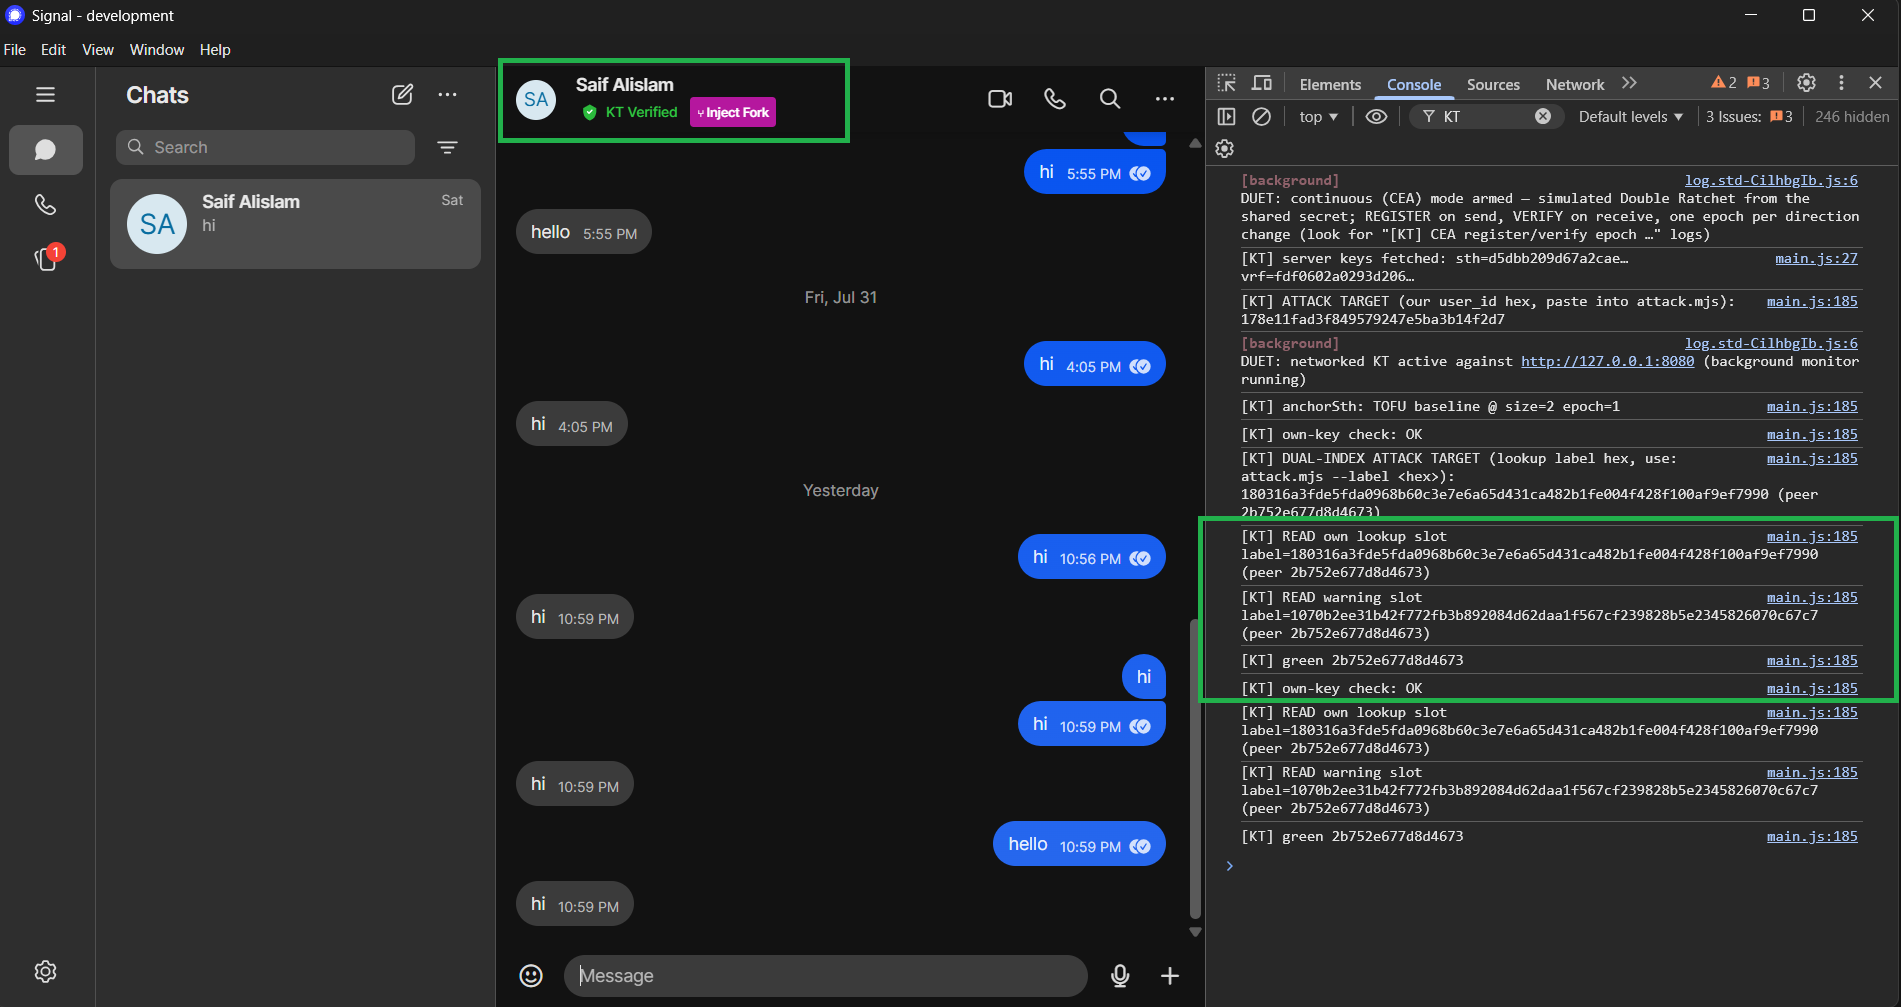
\includegraphics[width=\textwidth]{figures/normal.png}
\caption[Verified state before an attack.]{The client displays a verified state after successful
owner- and warning-slot checks.}
\label{fig:impl-baseline}
\end{figure}

\begin{figure}[p]
\centering
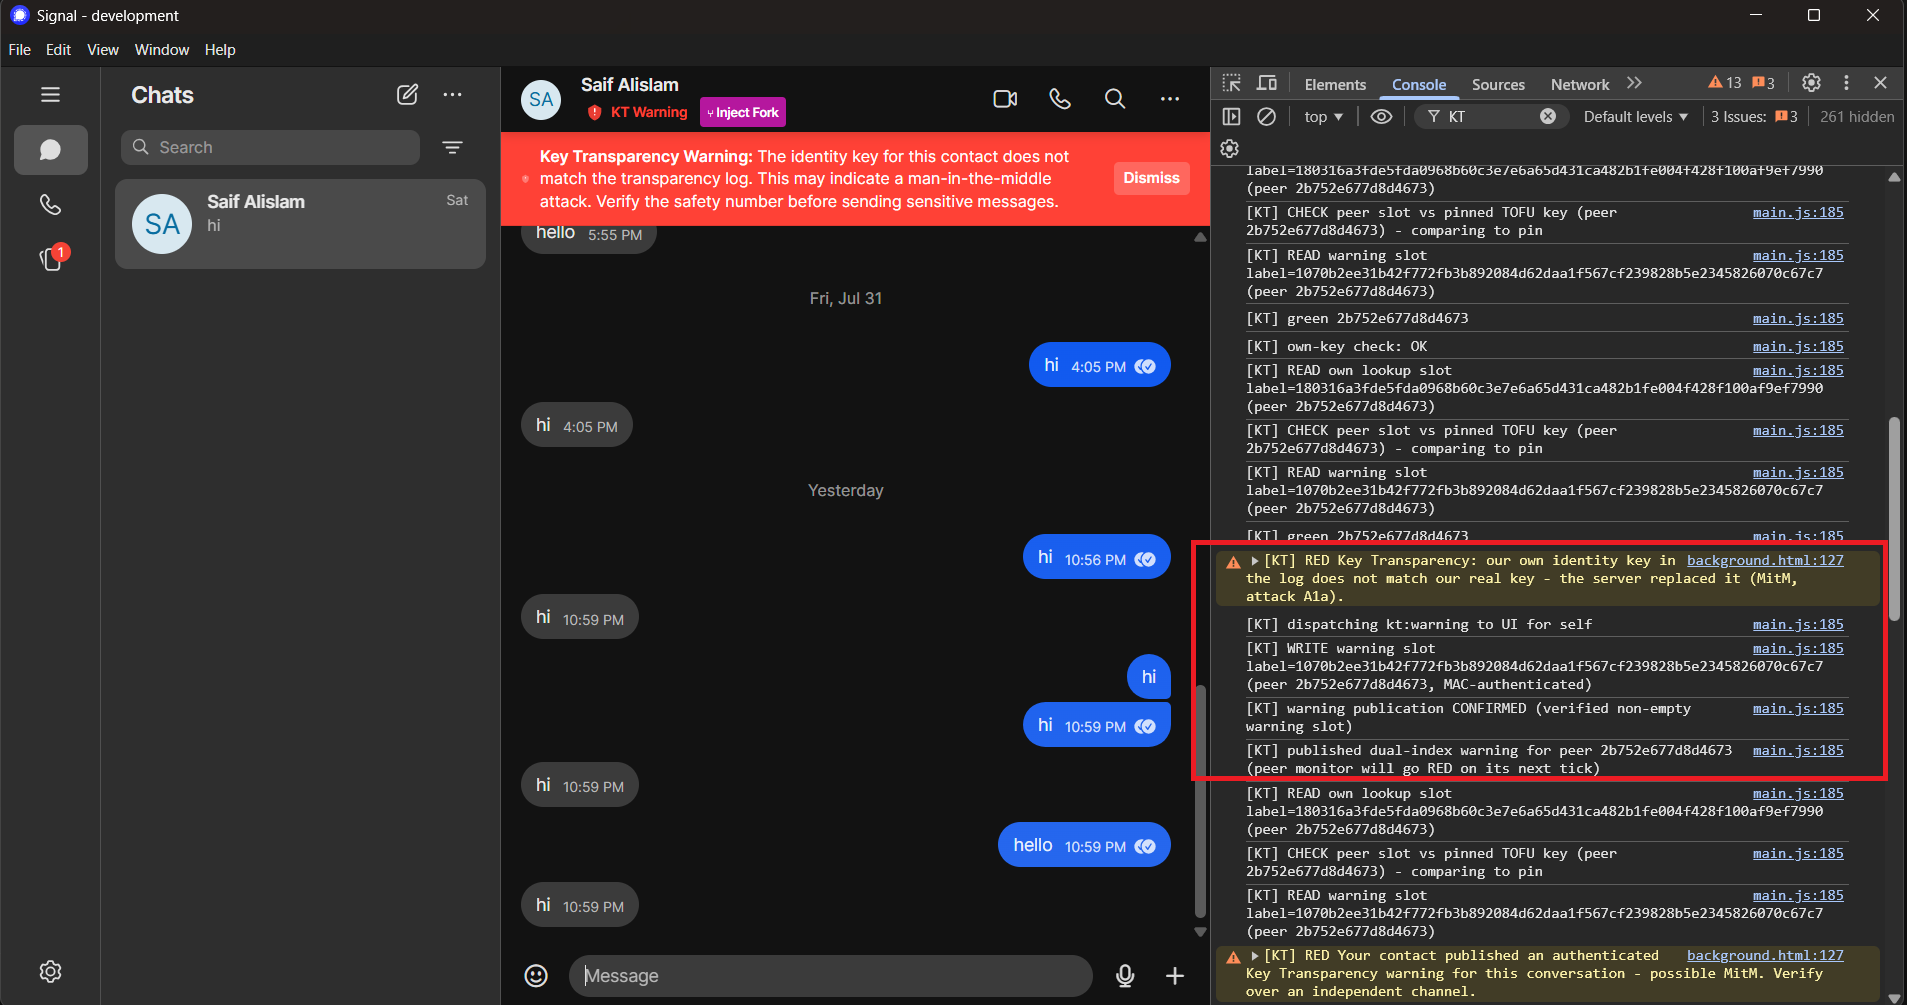
\includegraphics[width=\textwidth]{figures/attacked_user.png}\\[8pt]
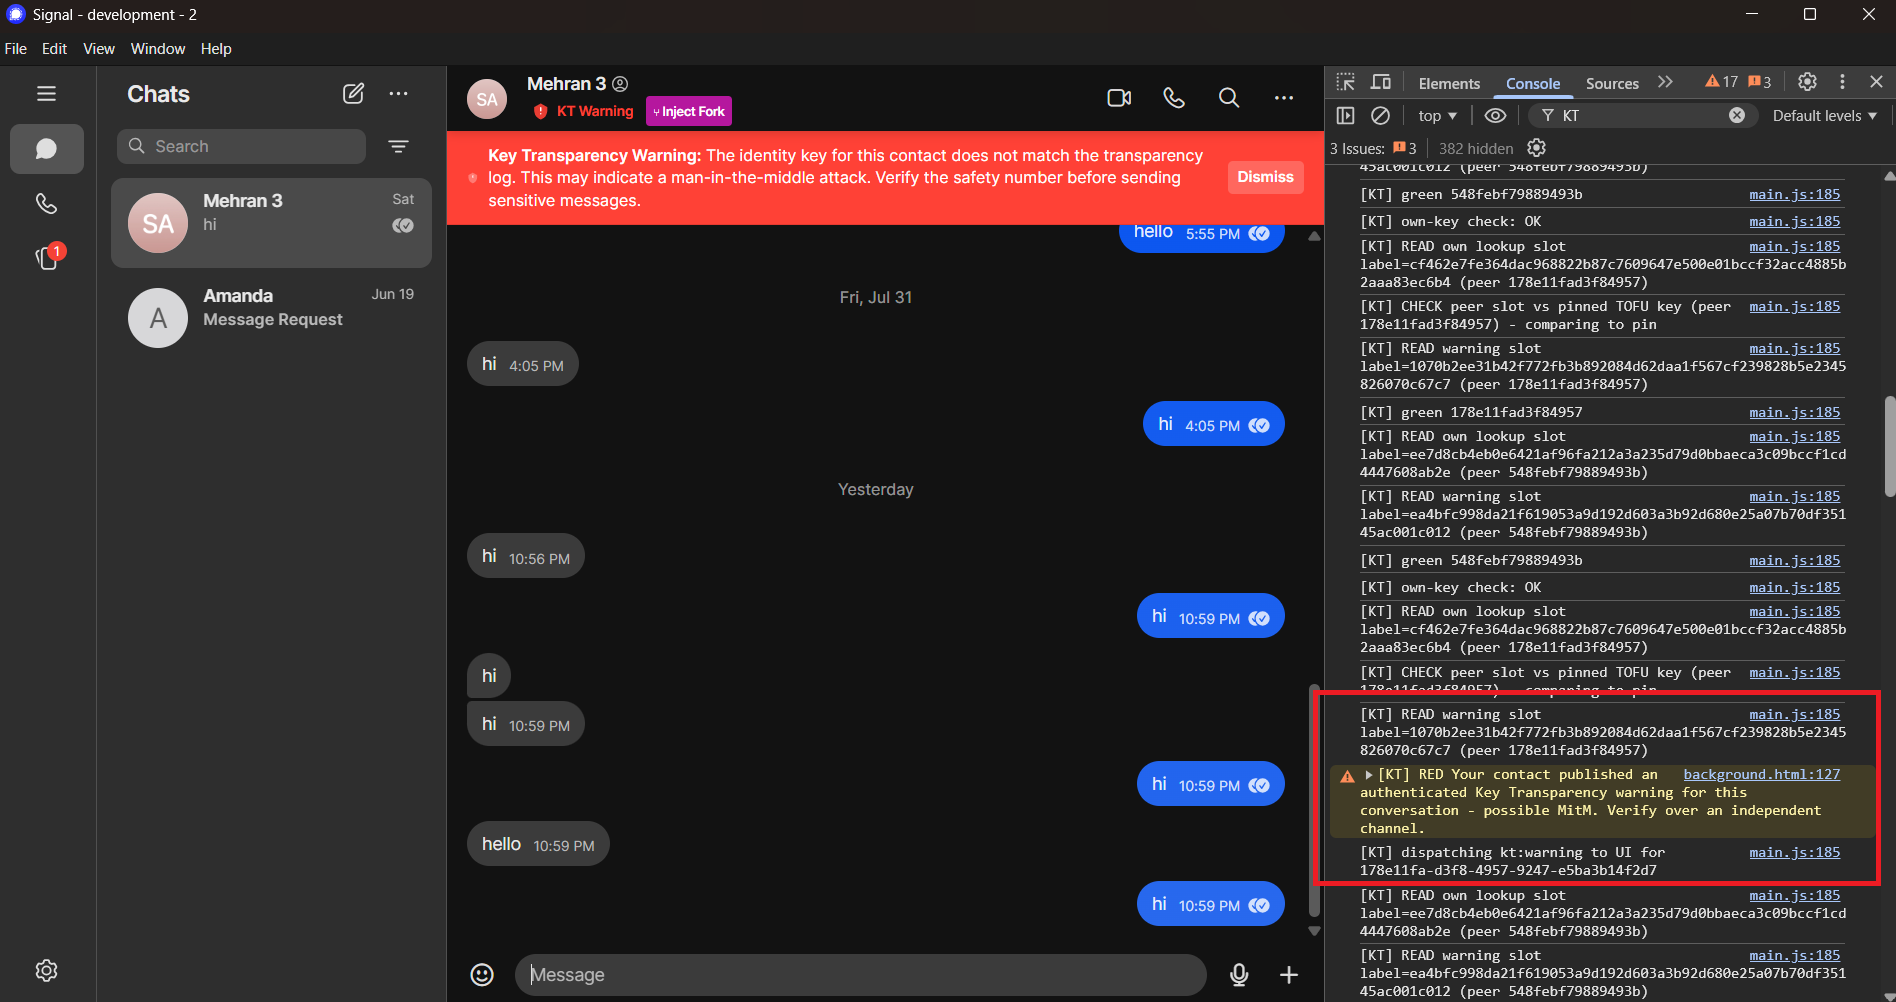
\includegraphics[width=\textwidth]{figures/peer.png}
\caption[Identity-slot warning on both clients (A1a).]{The affected client detects the substituted
identity key and publishes a warning. The peer verifies the shared warning, and both clients display
the red banner.}
\label{fig:impl-screens}
\end{figure}

% ============================================================================
\FloatBarrier
\section{Cross-Implementation Testing and Parity}\label{sec:impl-tests}

Testing connects the two implementations and the security claims. RFC vectors check the ECVRF. Fixed
cross-language vectors require byte-for-byte agreement for label derivation, warning payloads, and CEA
evolution. A live wire-parity suite checks the TypeScript verifier against signed heads, VRF outputs,
Merkle proofs, and consistency proofs produced by the Rust directory server. The Rust integration and
cryptographic suites run against a real in-process \texttt{KTServer} rather than a mock, and the
adversarial suite at \texttt{tests/adversarial.rs} covers A0,
\hyperref[sc:threat-a1]{A1a and A1b}, \hyperref[sc:threat-a2]{A2},
\hyperref[sc:threat-a3]{A3}, \hyperref[sc:threat-a4]{A4},
\hyperref[sc:threat-a5]{A5}, and \hyperref[sc:threat-x1]{X1}. These tests
establish agreement and expected behaviour for the specified inputs, not equivalence over every input.
The complete counts, names, and outcomes are in \cref{sec:tests-evidence}, within \cref{app:tests}.

The Rust tests exhaustively cover every Merkle-log
inclusion proof and every consistency pair up to size 64, together with forged-proof rejection, so the
log implementation is checked against its full input space at that size rather than at sampled points.
The auditor is tested for a soundness pair as well as a liveness one. A genuine equivocation is
reported as \textsc{Fork}, while a divergent head carrying an invalid signature is rejected outright
rather than misclassified as a fork.

The TypeScript harness contains 116 Jest tests, and sixteen further embedded tests run inside Signal
Desktop's own runner across four suites, exercising realistic account identifiers through the live
integration boundary. These totals are distinct from each other and from the opt-in live wire-parity
suite, and they must not be presented as one interchangeable figure.
\Cref{sec:impl-repro} records the complete reproduction commands and environment.

% ============================================================================
\FloatBarrier
\section{System-Wide Engineering Challenges}\label{sec:impl-challenges}

Three problems materially changed the implementation. First, the initial TypeScript label stand-in
could not agree with Rust's RFC~9381 ECVRF, because the two encode-to-curve steps differed. Both
clients were aligned on the ECVRF-EDWARDS25519-SHA512-TAI suite and checked against the published
vectors. Signed heads were also bound to each lookup response at this point, preventing a valid proof
from being paired with an unsigned or unrelated head.

Second, registration and lookup originally encoded Signal account identifiers differently. Converting
the service-ID string once at the integration boundary gives both paths the same canonical 16-byte
input and excludes phone-number identifiers before processing. Concurrent registration separately
exposed a time-of-check race between reading the head and using it to bound a proof. Binding each
consistency proof to the already validated head size prevents a later commit from making the client or
auditor compare a proof against the wrong upper bound.

Third, Electron bundling and context isolation prevented reliable loading and delivery to the
interface, through three distinct obstacles. The bundler split the key-transparency code at its
dynamic imports, so the layer was kept in one bundle. Context isolation blocked assignments to
\texttt{window} while allowing DOM custom events to cross the preload and renderer boundary. The
application's typed event bus and those DOM custom events were then mismatched, which was resolved by
dispatching on both. The remaining bundling, deterministic-state, and reset detail is preserved in
\cref{sec:apiref-engineering}.

Within the uncompromised-endpoint assumption in \cref{sec:threat-assumptions}, directory-response
verification relies on the verifier, its cryptographic dependencies, the hand-written ECVRF, and the
operator's two public keys, which are fetched once at initialization. The verifier returns a rejecting
verdict for invalid or absent signed heads, incorrect roots, missing inclusion proofs, mismatching labels,
and invalid VRF bindings. Availability
failures produce an amber notice rather than a red integrity warning, so an unreachable directory server is
never reported as an attack. The Signal hook currently reports these verdicts but leaves
session-blocking policy to future work.

Deterministic seeded server keys, a genesis epoch, and an administrative reset make the demonstration
repeatable and prevent a failed operation on an empty log from leaving the shared state unusable. A
poisoned mutex is likewise survivable in the harness. Production handlers would still need explicit
recovery from lock failure rather than relying on demonstration setup.

% ============================================================================
\section{Reproducibility}\label{sec:impl-repro}

Reproducibility of the measurements in \cref{ch:eval} depends on a recorded environment and
deterministic cryptographic and sampling inputs. Fixed seeds determine the VRF key, label placement,
and sampled users. Each benchmark begins from fresh seeded server state, so no residual state carries
between runs, while the live demonstration uses the administrative reset. The Rust tests and
benchmarks are run with \texttt{cargo test} and \texttt{cargo bench}, respectively. The environment
record captures the hardware, operating system, compiler, and toolchain versions. The repository
layout and the one-command runner scripts are listed in \cref{sec:apiref-repo}.

\chapter{Evaluation}\label{ch:eval}

This chapter evaluates the implementation described in \cref{ch:impl} against the requirements and
threats defined in \cref{ch:threat}. It examines proof size and verification cost, offline catch-up,
scalability, the trade-off between session and continuous modes, comparisons with prior systems, and
the coverage of the security controls.

% ============================================================================
\section{Methodology}\label{sec:eval-method}

The evaluation asks whether detection enlarges an individual proof, how verification changes with
directory size, and whether offline catch-up can use one proof. It also tests whether the defined
attacks are detected and the listed clean workflows complete without warnings. Seventeen metric families connect these
questions to proof size, latency, catch-up, scale, operating modes, and security outcomes.

The Rust harness measures local cryptographic work in process. It excludes HTTP, Electron, database,
and network costs. Manual-harness medians and 95th percentiles use \num{2000} sequential iterations,
while the scale experiment samples \num{1000} lookups per directory size. All DUET timings reported
in this chapter were measured on the Windows x86\_64 host described in \cref{sec:bench-env} (12th Gen
Intel Core i7-12700H, 31.7\,GB RAM). Under the worked parameterization of
\cref{ssec:design-param}, epochs are hourly, so a window of $W=720$ epochs spans 30 days. Proof sizes are exact for the recorded
seeds. Values near timer resolution are treated as coarse observations. Cross-system timing comparisons
are approximate because the published implementations and hardware differ. \Cref{app:benchmarks} defines the metric families
and baseline configurations and provides the complete tables, measurement environment, and
reproduction instructions.

% ============================================================================
\section{Measured Results}\label{sec:eval-micro}

The following subsections present the measured proof sizes and verification costs, offline catch-up
results, and detection-path costs. Each result is stated with the scope of its measurement.


\subsection{Proof Size and Verification (M1--M3, M14)}\label{ssec:eval-sizes}\label{ssec:eval-latency}

A lookup proof carries a prefix copath, a log-inclusion path, and fixed VRF and framing fields. For a
VRF-indexed lookup, its serialized proof body is modelled as:

\begin{equation}\label{eq:eval-proofsize}
  |\pi| \;=\; 32h \;+\; 32h_{\mathrm{log}} \;+\; 177 \ \text{bytes},
  \qquad \mathbb{E}[h]\approx\lceil\lg N\rceil,\quad h_{\mathrm{log}}\le\lceil\lg E\rceil,
\end{equation}

where $h$ is the number of non-empty siblings on the queried label's path and $h_{\mathrm{log}}$ is
the log-inclusion path length. The \num{177}-byte constant comprises the \num{80}-byte ECVRF proof, a
label, a value, a leaf-kind commitment, and a sibling bitmap. Raw-label warning responses omit the VRF
component. The median lookup proof is \num{817} bytes at $N=10^{6}$ and \num{945} bytes at
$N=10^{7}$, and the growth between them is the $\lceil \lg N \rceil$ term, not any change in the
fixed component. The full component breakdown and distribution table are in \cref{sec:bench-sizes}.

Detection does not change this format. A dual-index or CEA check performs another lookup against the
same directory and signed head without enlarging an individual proof.

M14 isolates the history-depth term. Across $E\in\{1,16,256,1024\}$, log inclusion adds
\num{0}, \num{128}, \num{256}, and \num{320} bytes, matching the
$32\lceil\lg E\rceil$ bound. Median full verification remains below
\SI{150}{\micro\second} throughout the grid and reaches at most
\SI{143.2}{\micro\second}. Directory size and history depth therefore contribute independently to
the measured proof size.

Full client verification, which covers the VRF, the log inclusion path, and the signed head, has a
median of \SI{128.7}{\micro\second} at $N=10^{3}$ in the manual harness. Within the scale experiment
(\cref{tab:bench-scale}), the median rises from \SI{133.6}{\micro\second} at $N=10^{6}$ to
\SI{139.2}{\micro\second} at $N=10^{7}$, an increase of \SI{5.6}{\micro\second}, or 4.2 percent, for a
tenfold larger directory. The result supports slow growth relative to directory size. Prefix-only
verification moves from \SI{26.3}{\micro\second} to \SI{26.4}{\micro\second} over the same range,
accounting for little of the full-verification increase. The benchmark does not isolate the remaining
cause.

The 95th-percentile tail for server-side search at $N=10^{7}$ remains unexplained. It is
\SI{4581.9}{\micro\second}, compared with a median of \SI{441.7}{\micro\second}
(\cref{tab:bench-scale}). The harness did not record
operating-system paging activity, so the benchmark cannot determine whether memory pressure caused the
tail. The tail is reported as observed implementation behaviour, without assigning an unmeasured cause.

\subsection{Offline Catch-Up (M4)}\label{ssec:eval-catchup}

A client that has been offline for a window of $W$ epochs must establish that the head it now sees is
consistent with the head it last verified. The windowed construction answers this with one proof
rather than one proof per epoch. At $W = 720$ the windowed proof is \num{320} raw hash bytes against
\num{222528} bytes for the synthetic repeated-proof baseline, a ratio of \num{695.4}.
\Cref{fig:eval-catchup-plot} shows how the two curves separate as the window grows. The baseline is
synthetic and is constructed by repeating the implemented single-epoch proof, so it measures what
this system would cost without windowing, not what any deployed system does cost. Both figures
count raw path hashes and not serialized network traffic. Verifying adjacent epoch transitions would
use smaller individual proofs, so the exact ratio is specific to this baseline even though the
one-proof-versus-$W$-proof comparison remains. Generation timings for the same experiment
are in \cref{sec:bench-sizes}. This addresses the monitoring-bandwidth extension identified by
CONIKS~\cite{melara2015coniks}.

\begin{figure}[ht]
\centering
% fig-eval-catchup-plot.tex — extracted from ch6-evaluation.tex
% Label: \label{fig:eval-catchup-plot}
\begin{tikzpicture}
\begin{axis}[width=0.74\textwidth,height=6cm,xmode=log,ymode=log,
  xlabel={offline window $W$ (epochs)}, ylabel={raw consistency-path hash bytes},
  xtick={1,24,168,720}, xticklabels={1,24,168,720}, log ticks with fixed point,
  legend style={at={(0.5,-0.30)},anchor=north,legend columns=1,font=\scriptsize},
  grid=both, font=\footnotesize]
\addplot+[mark=*] coordinates {(1,96)(24,4416)(168,41280)(720,222528)};
\addplot+[mark=square*] coordinates {(1,96)(24,192)(168,256)(720,320)};
\legend{synthetic current-head baseline ($W$ proofs), windowed (one proof)}
\end{axis}
\end{tikzpicture}

\caption[Catch-up bandwidth versus offline window.]{Raw consistency-path hash bytes for offline
catch-up versus window $W$, shown on a logarithmic vertical axis. The synthetic
current-head-anchored baseline grows linearly to \num{222528} bytes at one month. The windowed
proof remains a few hundred bytes and grows logarithmically (\cref{sec:bench-sizes}).}
\label{fig:eval-catchup-plot}
\end{figure}

\subsection{Detection Costs and Clean-Run Results (M16, M17)}\label{ssec:eval-detection}

A verified lookup whose returned owner does not match the expected owner completes in
\SI{27.8}{\micro\second}. The clean two-lookup path fetches and verifies both the self label and the
peer label and completes in \SI{31.1}{\micro\second}. These Rust reconstructions measure local
verified-lookup work in the mismatch and clean paths. They exclude the TypeScript client, transport, polling,
and registration, so they bound the local cryptographic component and do not represent user-visible latency.

All seven specified clean workflows produce their expected clean verdicts (\cref{tab:bench-m17}), and no workflow produces a
warning. The security outcomes are treated in \cref{sec:eval-security}.

% ============================================================================
\section{Scalability, Maintenance, and Authentication Modes}\label{sec:eval-scale}

\subsection{Scale, Maintenance, and Auditing (M7, M9, M12)}\label{ssec:eval-scale}\label{ssec:eval-throughput}\label{ssec:eval-auditor}

Rotation costs between \SI{138.7}{\micro\second} and \SI{140.3}{\micro\second} across the measured
sizes, which is consistent with a fixed-cost VRF dominating the per-label work, not any
dependence on directory size. Epoch commit moves from \SI{451.0}{\micro\second} at $N=10^3$ to
\SI{6.73}{\milli\second} at $N=10^4$. The increase is caused by deep-cloning the current tree into the committed snapshot, not the tree update itself. These two points do not establish an asymptote, but they identify epoch commit as the component
most likely to require engineering attention at deployment scale.

Building the $N=10^{7}$ directory takes about 26 minutes at \SI{21.3}{\giga\byte} resident set on the
evaluation host. The single-process research build holds the whole directory in memory behind one
mutex, making memory use a primary deployment constraint.

M12 measures two local verification operations, not a complete networked audit. The first combines an
STH signature check with consistency-proof generation and verification. Its median is
\SI{28.6}{\micro\second}. This includes proof generation but excludes transport, replay, scheduling,
persistence, and the cross-vantage comparison required by a deployed audit. The second checks for a fork
against one observed head. Its median is \SI{27.1}{\micro\second}, and its 95th percentile is
\SI{33.1}{\micro\second}.

\subsection{Session and Continuous Modes (M13, M15)}\label{ssec:eval-modes}

Session mode and continuous mode show similar isolated label-bound verification cost, at
\SI{27.3}{\micro\second} and \SI{27.7}{\micro\second}. The difference is within run-to-run variation
and no ordering between the two is inferred from it. Verification cost is also stable in the number
of catch-up epochs replayed, varying by at most \SI{0.5}{\micro\second} over
$K \in \{1, 10, 100, 720\}$.

The two modes have similar isolated verification costs, but their write cadences differ. Session mode writes once per
signed-pre-key rotation, while continuous mode writes once per ratchet epoch. At $R = 720$ the
modelled write counts differ by factors between 24 and 720 depending on the modelled number of epochs.
That ratio is a property of the cadence model and the simulated input, and it is not a deployment
bound. The full mode table is in \cref{sec:bench-modes}.

% ============================================================================
\section{Comparison with Prior Systems}\label{sec:eval-compare}

The published systems use different implementations, hardware, and accounting conventions. Each
comparison below therefore states the matched components and arithmetic.
\Cref{tab:eval-compare} summarizes the resulting trade-offs.

\begin{table}[H]
\centering
\caption{DUET compared with prior systems using published figures.}
\label{tab:eval-compare}
\footnotesize
\begin{tabularx}{\textwidth}{@{}>{\raggedright\arraybackslash}p{2.5cm}>{\raggedright\arraybackslash}X>{\raggedright\arraybackslash}X>{\raggedright\arraybackslash}X@{}}
\toprule
Dimension & DUET (measured) & CONIKS~\cite{melara2015coniks} & Signal KT~\cite{signal-kt-server} \\
\midrule
Lookup proof size & 817\,B median at $10^6$ (max 945, prefix and VRF, excluding STH) & 1{,}216\,B at $2^{32}$, 768--832\,B at $10^6$ derived (proof with and without signature) & 8{,}192\,B fixed sibling copath only (256$\times$32, no VRF) \\
Client lookup verification & $\approx$\SI{128}{\micro\second} at $10^3$--$10^4$, \SI{139.2}{\micro\second} at $10^7$ (including VRF and signed-head verification) & \SI{159}{\micro\second} for path verification at $10^7$ and approximately \SI{400}{\micro\second} for signature verification, giving a derived total of about \SI{559}{\micro\second}, excluding VRF & not published \\
Catch-up at $W{=}720$ & 320\,B (1 windowed proof) & $\Theta(W)$, $\sim$530\,kB derived & Monitoring endpoint\newline No published byte figure \\
Key-substitution detection & automatic in-band peer warning (established conversations)\newline global VRF-bound identity check, honest directory (first contact) & manual Safety Number comparison and self-monitoring & optional AKV lookup and self-monitoring\newline no peer warning \\
Authenticated records & Identity-key bindings at global and session-derived slots, and per-epoch ratchet-key fingerprints in continuous mode & Identity-key bindings & Account-identifier, phone-number, and username-hash mappings \\
Query privacy (operator) & No & No & No \\
Resists offline identity recovery (VRF) & Yes (ECVRF, 80\,B) & Yes (discrete-log-based VRF, 96\,B) & Yes (ECVRF) \\
\bottomrule
\end{tabularx}
\end{table}

At $N = 10^{6}$ a CONIKS lookup proof carries a 21-node authentication path, an index or commitment
component, and a signature, which gives $32 \times 21 + 96 + 64 = 832$ bytes, or 768 bytes excluding
the signature~\cite[Section~5.3, Table~1]{melara2015coniks}. DUET's \num{817}-byte median is measured
excluding the signed head, so 768 bytes is the matched quantity, and DUET is within 7 percent of it.
The two systems are therefore in the same size class for an individual lookup, and DUET's detection
capability does not enlarge that individual proof format.

Signal's deployed verifiable key directory verifies a fixed-length prefix copath. Its
\texttt{evaluateProof} routine in \texttt{tree/prefix/verify.go} requires exactly 256 siblings, which
is $256 \times 32 = 8{,}192$ bytes~\cite{signal-kt-server}. Against DUET's \num{817}- and
\num{945}-byte medians the
ratios are 10.0 and 8.7. The difference reflects a trade-off rather than a strict improvement. The fixed-length copath
reveals nothing about how populated the tree is, whereas DUET's bitmap compression exposes
approximately $\lceil \lg N \rceil$ bits of density metadata to whoever holds the proof. DUET
trades that bounded metadata exposure for lower bandwidth. SEEMless reports approximately
8.6\,\si{\kilo\byte} at $N = 10^{7}$ under its own construction~\cite[p.~12]{chase2019seemless}, close
to Signal's fixed \num{8192}-byte copath. The figures are not directly comparable because the
constructions account for different proof components.

For offline catch-up the difference is larger. CONIKS reports an approximately 736-byte per-epoch
proof~\cite[Section~5.3]{melara2015coniks}, so a 720-epoch window costs $720 \times 736 = 529{,}920$
bytes against DUET's \num{320}-byte windowed proof, a ratio of approximately 1{,}656. CONIKS
prescribes a separate proof of the client's binding for every missed epoch. DUET's \num{320}-byte
figure measures the returning client's consistency proof. Peer warnings and transition auditing are
separate mechanisms, and their costs are excluded from this ratio.

For client verification, CONIKS reports a \SI{159}{\micro\second} path verification and an approximately
\SI{400}{\micro\second} signature verification~\cite[Section~5.3]{melara2015coniks}, giving a derived
total of about \SI{559}{\micro\second}. CONIKS publishes no separate VRF timing, so that component is
absent from the total. The matched DUET figure is the \SI{139.2}{\micro\second} full verification at
$N=10^{7}$, aligning the comparison at a large directory size. The proof-size comparison excludes
signed heads and signatures on both sides. The timing comparison includes them on both sides. DUET's
figure includes signed-head verification, and the CONIKS total includes its reported signature
verification.

\begin{quote}\small\noindent\textbf{Comparability note.}
The figures above are drawn from published results measured on different hardware, with different
implementations, and under different workloads. They provide broad context and locate DUET within the
design space. They are not a controlled benchmark, and no claim of superiority
on any dimension other than the stated arithmetic is made.
\end{quote}

% ============================================================================
\section{Security Evaluation}\label{sec:eval-security}

The adversarial suite includes tests for the scenarios defined in \cref{ch:threat}: the honest baseline
A0, key substitution (\hyperref[sc:threat-a1]{A1a and A1b}), warning censorship
(\hyperref[sc:threat-a2]{A2}), network man-in-the-middle (\hyperref[sc:threat-a3]{A3}), split-view
equivocation (\hyperref[sc:threat-a4]{A4}), malicious rotation (\hyperref[sc:threat-a5]{A5}), and the
excluded endpoint-compromise case (\hyperref[sc:threat-x1]{X1}). \Cref{tab:eval-security} summarizes
the attack families, their controls, and the observed outcomes. \Cref{tab:tests-adversarial} records
each scenario individually, and \cref{tab:bench-m17} records the seven clean workflows. Every scenario
produces its expected outcome, and the clean workflows produce their expected clean verdicts with no
warnings.

The test schedule performs one action per epoch, so the table's epoch counts describe the harness
rather than detection latency. The outcomes hold under the assumptions defined in
\cref{sec:threat-assumptions}, in particular an uncompromised endpoint and an auditor with an
independent vantage.

\begin{table}[ht]
\centering
\caption{Evaluated threats, detection controls, evidence, and outcomes.}
\label{tab:eval-security}
\footnotesize
\renewcommand{\arraystretch}{1.3}\setlength{\extrarowheight}{3pt}
\begin{tabularx}{\textwidth}{@{}>{\raggedright\arraybackslash}p{2.0cm}>{\raggedright\arraybackslash}p{3.5cm}X>{\raggedright\arraybackslash}p{3.6cm}@{}}
\toprule
Case & Control and requirement & Evidence & Result \\
\midrule
Key substitution (\hyperref[sc:threat-a1]{A1a and A1b}) & Owner self-check and dual-index warning (G1). & \cref{tab:tests-adversarial}. & Detected. \\
\hyperref[sc:threat-a3]{A3} network MitM postcondition & Global VRF-bound identity check, honest directory (G1). & \cref{tab:tests-adversarial}. & Detected at the next lookup. \\
\hyperref[sc:threat-a5]{A5} malicious rotation & Identity re-fetch and predecessor cross-signature (G1). & \cref{tab:tests-adversarial}. & Detected. \\
\hyperref[sc:threat-a2]{A2} warning censorship & Pre-commit key mismatch with proof-verified warning absence, and post-commit removal caught as an invalid transition (extension of G1). & \cref{tab:tests-adversarial}. & Detected. \\
\hyperref[sc:threat-a4]{A4} split-view equivocation & Cross-vantage auditor (G4). & Equivocation test and the M12 signed-head fork comparison. & Detected at the next comparison. \\
\midrule
Offline identity recovery from published labels (G3) & ECVRF-derived labels resist offline recovery of identities by traversing public labels (G3). & VRF assumption. RFC~9381 vectors check implementation conformance (\cref{tab:tests-rust-prim}). & Resisted offline under the VRF assumption. The public query endpoint still permits online membership tests. \\
\hyperref[sc:threat-x1]{X1} key extraction & No directory control. & Endpoint compromise lies outside key transparency. & Out of scope. \\
\bottomrule
\end{tabularx}
\end{table}

The supporting analysis maps the scenarios to STRIDE~\cite{stride} in
\cref{sec:sec-stride}, MITRE ATT\&CK~\cite{mitre-attack} in \cref{sec:sec-mitre},
and the attack routes in \cref{sec:sec-routes}, while \cref{ssec:eval-timeline}
gives the detection sequence.

\subsection{Residual Risks and Security Position}\label{ssec:eval-posture}

A rejecting verdict shows that an integrity or consistency check failed without identifying its cause
or attributing it to the directory operator. An unavailable directory server raises an amber notice,
while a verified mismatch or the fail-closed operational timeout raises a red
warning. Endpoint compromise defeats every mechanism evaluated here because the verifier and the keys
it trusts live on the endpoint.

% ============================================================================
\section{Implications for Deployment}\label{sec:eval-deploy}

The measured client costs support the feasibility of client-side verification at the tested scale:
median full verification stays below \SI{150}{\micro\second} through $10^7$ labels, the proof body
stays below one kilobyte, and detection reuses this format through additional label-bound lookups
without enlarging an individual proof.

Offline catch-up uses one proof for the missed window. At $W=720$, its \num{320} raw hash bytes
compare with \num{222528} bytes across \num{720} proofs for the synthetic repeated-proof baseline.
Both figures exclude serialization overhead. The baseline models this implementation without
windowing, not a deployed system.

M16 measures the Rust lookup work for the mismatch path and the clean two-lookup path. These
component timings exclude network transfer and end-to-end background-monitor latency. The directory server measurements expose two
further constraints. Epoch commit deep-clones the current tree into the committed snapshot, and the
in-memory tree becomes large at $10^{7}$ entries. Persistent structural sharing, storage, concurrency
testing, and networked measurements remain necessary.

Session and continuous modes have similar isolated verification costs but different write frequencies.
Their measured ratio reflects the cadence model, not a fixed deployment value.

\chapter{Discussion, Limitations and Future Work}\label{ch:discussion}

This chapter interprets the results, states the prototype's limitations, and identifies priorities for
completing, deploying, and extending the system.

% ============================================================================
\section{Discussion}\label{sec:disc-discussion}

DUET adds automatic in-band substitution detection through additional label-bound lookups rather than
a new proof family, so it preserves the lookup proof's asymptotic size and verification cost. The
guarantee depends on domain-separated labels, proof-verified absence, warning persistence, and
transition validation. Under \hyperref[sc:threat-a3]{A3}, divergent conversation secrets produce different labels, while the
global VRF-bound identity entry supplies an independent binding.

The evaluation supports this separation of costs. Identity proofs remain roughly comparable with the
matched CONIKS proof, detection paths reuse raw-label proofs, and distant-head consistency replaces
a proof per missed epoch with one proof. These measurements characterize component costs rather than
production throughput.

The construction applies beyond Signal wherever a messenger supplies a semi-trusted directory and a
conversation secret, with continuous mode additionally needing public ratchet keys and secret epoch
inputs. Session mode has the smaller integration and write surface, while continuous mode
authenticates each ratchet epoch at a higher write rate. Both remain bounded by trust on first use,
endpoint security, and the need for an independent vantage to expose a consistent fork.

% ============================================================================
\section{Limitations}\label{sec:disc-limitations}

The guarantee begins only after a baseline has been pinned, so it cannot establish whether the
initial binding was authentic. It covers
pairwise, single-device conversations rather than groups, MLS, Sender Keys, or complete multi-device
warning propagation. Endpoint compromise remains outside any directory guarantee.

Transition auditing requires an honest auditor, and \hyperref[sc:threat-a4]{A4} additionally requires a valid signed head from
an independent vantage. A client alone rejects a head that does not extend its pinned baseline, but
it cannot expose two internally consistent branches extending a common prefix. Production deployment
also needs authenticated epoch disclosures, freshness and failure policies, and a real gossip or
second-vantage source.

The prototype provides no query privacy from the operator, write-rate limit, published-head timeout,
or gossip-based proof-omission detection. A malicious peer can publish a valid but false warning,
since the payload MAC authenticates the peer rather than the truth of its report, so attributable
warning records and abuse policy remain necessary.

The implementation is single-machine and in-memory, and epoch commit deep-clones the current tree into
the committed snapshot. The Signal client uses a deterministic conversation-secret stand-in and a
seeded ratchet simulation, which exercise the code
paths but do not establish label unpredictability or active-attacker security for live Signal state.
The key-fetch hook reports a rejecting verdict without blocking session establishment. The simulated
continuous mode supplies the raw Diffie--Hellman output where ACKA's Signal mapping uses the derived
chain key, and its synchronous state does not model skipped ratchet epochs. A faithful binding must
obtain the live chain key and support explicit epoch indices and bounded skipped state.

The security argument is an informal proof sketch supported by definitions, the same-head lemma, and
the adversarial suite. The suite does not model separate first-contact sessions with each party or a
fabricated pre-key bundle kept consistent with a malicious directory entry. Timings measure local
components rather than a complete networked monitor or audit, and the committed corpus contains
aggregate statistics rather than raw Criterion samples. M11 repeats the Rust lookup-verification
component rather than timing the TypeScript key-fetch path, and M12 measures local signature and
consistency work rather than network transfer, epoch-delta retrieval, or full transition replay.
These distinctions prevent the component evidence from being read as an end-to-end deployment
measurement.

% ============================================================================
\section{Future Work}\label{sec:disc-future}

\subsection{Completing the Protocol and Security Argument}

The first implementation priority is to obtain the live X3DH or PQXDH conversation secret and the
live Double Ratchet chain key from libsignal. Replacing the stand-ins changes the inputs to the
existing label and CEA constructions rather than their downstream proof formats. The live
conversation secret is required for the \hyperref[sc:threat-a3]{A3} label-unpredictability claim. The
raw-label interface must also authenticate the party authorized to make the first write, preventing a
malicious client from occupying an empty conversation slot before its legitimate owner. Later
replacement and deletion remain governed by transition auditing rather than first-write
authorization. The tested persistence component provides evidence of later removal, and its
implementation status is identified in \cref{tab:impl-modules}. A formal analysis should define a
combined detection game covering the KDF, VRF, signed heads, warning authentication, and append-only
verification, alongside symbolic analysis and separate verification of the client proof checker.

\subsection{Groups, Devices, and Directory Privacy}

Group support requires epoch-scoped labels and a
warning policy for joins, removals, and every current device, potentially using domain-separated MLS
exporter secrets~\cite{rfc9420}. ELEKTRA-style device cross-signing could strengthen multi-device
continuity~\cite{len2023elektra}, alongside device-scoped labels, warning propagation, and reset
handling. OPRF-based identity blinding could hide the raw lookup identity, but private retrieval and
network anonymity would still be needed to conceal the fetched entry and the requester, and the
design would have to define how the OPRF role is separated or distributed~\cite{rfc9497}.

\subsection{Deployment and Cryptographic Scale}

Persistent copy-on-write nodes should replace full
snapshot cloning. With fixed depth $d=256$, copying the paths for $k$ modified labels is $O(kd)$ and
therefore $O(k)$, independent of $N$. The proof format would remain unchanged. Building on Signal's
existing key-transparency service~\cite{signal-kt-server} would additionally
require immutable raw writes, authenticated ownership, transition disclosures, client hooks, and an
independent auditor or gossip federation with incentives for independent operation. PQXDH secrets
already fit the label KDF, but post-quantum operation also needs replacements for the ECVRF and
signed-head signatures~\cite{pqxdh}. This thesis does not select or implement a post-quantum VRF.
Even with PQXDH-derived labels, end-to-end post-quantum security would still depend on the messenger's
authentication and ratchet mechanisms. Concurrency, serialization, reclamation, and memory use would
require measurement after structural sharing.

\subsection{Evaluation, Operations, and Usability}

A usability study should determine whether cryptographic detection leads to an appropriate user
response. It should test interpretation of the red warning and amber notice, accessibility,
escalation, and alarm fatigue, continuing the ceremony research that motivated the
design~\cite{vaziripour2017}. Production warnings
should carry the scenario, epoch, signed heads, and proofs needed for operator or auditor review
without exposing unnecessary metadata. An operational policy must define when to reject a proof,
request rotation, or escalate without turning warning records into a new metadata leak. Further
experiments should use persistent storage, concurrent requests, wide-area delay, varied epoch and
catch-up policies, mobile CPU and energy measurements, and archived raw samples. The same approach
may also be evaluated in clinical, emergency-response, and industrial key-distribution settings, each
with its own identity model, device-enrolment and revocation process, availability requirements, and
regulatory controls.

\chapter{Legal, Social, Ethical and Professional Issues}\label{ch:lsepi}

This project builds security-critical infrastructure for a widely used messaging application, and
it does so by modifying deployed open-source software; both facts carry legal, social, ethical, and
professional obligations. This chapter sets out those obligations and how they were discharged
during the work. It considers the legal position of the code and the data
(\cref{sec:lsepi-legal}), the social and ethical implications of strengthening, and of being
seen to strengthen, end-to-end-encrypted messaging (\cref{sec:lsepi-social}), and the
professional standards, specifically the BCS Code of Conduct~\cite{bcs-code} and the IET Rules of
Conduct~\cite{iet-conduct}, against which the work was conducted (\cref{sec:lsepi-prof}).

% ============================================================================
\section{Legal Issues}\label{sec:lsepi-legal}

Intellectual property and licensing are the most immediate legal consideration. The prototype
extends two Signal codebases, libsignal and Signal Desktop, both released under the GNU
Affero General Public License v3 (AGPL-3.0)~\cite{libsignal,signal-desktop}. The project is
distributed on the basis that modifications to the AGPL-covered Signal code remain under AGPL-3.0:
their source must remain available, and, distinctively for the AGPL, that obligation extends to
users who interact with a modified version over a network, not only to those who receive a binary.
Whether a particular separately developed component is itself a derivative work can depend on the
facts, the jurisdiction, and the mode of combination and distribution. The prototype is a
research artefact rather than a deployed service, so no public network offering has been made; but
the licence terms have been respected throughout: the modifications are kept in a fork whose
source is available, the upstream copyright and licence notices are preserved, and any future
deployment of the modified Signal code would carry the same AGPL-3.0 obligations, including the
network-interaction source requirement. The independent Rust \texttt{duet} crate depends on
permissively licensed libraries, including \texttt{sha2} and \texttt{hkdf} (MIT/Apache-2.0)
and \texttt{curve25519-dalek} and \texttt{ed25519-dalek} (BSD-3-Clause), all compatible with that
outcome. All third-party work (specifications, prior systems, and code) is attributed in the
references.

A second consideration is export control. The work implements cryptographic software, which is
regulated under the Wassenaar Arrangement and national export regimes; libsignal itself is
published under the corresponding open-source exception for publicly available cryptographic source
code. The contribution composes standardized primitives
(the RFC~9381 ECVRF, RFC~5869 HKDF, and Ed25519) without introducing new cryptographic algorithms, and is released as open, published source. This
thesis does not determine the software's export-control classification: public availability may be
relevant, but the applicable control lists and end-use rules require a case-specific assessment.

Data protection is the third. Key transparency is, by construction, a data-minimizing design: the
directory stores public keys and pseudonymous labels, never message content, and the VRF-derived
global labels (\cref{ssec:design-labels}) deliberately prevent an observer from enumerating which
users are present. The benchmark corpus used generated identifiers not linked to identifiable
individuals. Subject to that assumption, the benchmark data were not personal data and no
obligations under the UK GDPR were engaged by the measurements, while the design itself advances the
privacy interests that data-protection regimes exist to protect. Screenshots and operational logs that contain
identifiable names or paths would require separate review before release. A
production deployment would inherit one governance duty the prototype does not: any operational
logging of warnings or audit events must itself be data-minimized and access-controlled, so that
the alerting layer does not re-expose the label-to-user metadata the pseudorandom labels are
designed to hide.

% ============================================================================
\section{Social and Ethical Issues}\label{sec:lsepi-social}

The social value of the work is a direct contribution to public wellbeing and security:
authenticated key exchange is what makes end-to-end encryption meaningful, and the people who most
depend on it (journalists, activists, and others at risk) are exactly those whom an
undetected key substitution would endanger. Strengthening the automatic detection of such attacks,
and giving both conversation partners an in-band warning, serves the public interest that the BCS
code places first.

That same importance imposes a duty of honesty about what the work does and does not achieve,
because a security tool trusted beyond its guarantees is worse than none. The thesis is explicit
about its limitations: the prototype carries two proof-of-concept stand-ins for live protocol state
(\cref{sec:impl-strategy}), it is a single-machine prototype rather than a distributed deployment,
and the boundary case of key extraction is out of scope (\cref{ch:threat}). The user-facing design
embodies the same caution: an unreachable server raises a calm, amber notice rather than the red
alarm reserved for a detected attack (\cref{ssec:impl-verifier}), precisely so that the system does
not ``cry wolf'' and erode the trust its warnings depend on. The design is open and
specification-grounded rather than security-through-obscurity, and its correctness is evidenced by
reproducible tests against published vectors (\cref{sec:impl-tests}) rather than asserted.

A dual-use dimension is unavoidable: strong messaging security protects everyone, including those
who would misuse it. This project treats defensive integrity infrastructure of this kind as serving the public good,
since weakening it to disadvantage bad actors would also weaken protection for the far larger
population of ordinary and at-risk users; the professional codes cited in \cref{sec:lsepi-prof}
support this position. Finally, the work followed responsible-disclosure norms in the small: the one
security-relevant weakness found during integration, a per-lookup head-binding gap, was in
the author's own prototype and was fixed (\cref{sec:impl-challenges}); no vulnerability in deployed
Signal software was discovered, but had one been, the appropriate course would have been private
disclosure to Signal before any publication.

A warning mechanism also has direct effects on the people who see it, which a responsible design must
weigh. Because the channel can be written by a peer, a malicious or compromised contact can raise a
spurious warning; at scale, frequent or unexplained alerts risk \emph{warning fatigue}, in which users
learn to dismiss the very signal meant to protect them (\cref{sec:disc-limitations}). The design
mitigates this by distinguishing a genuine integrity alert (red) from mere unavailability (amber) and
by deriving the warning from cryptographic evidence rather than heuristics, but the wording, frequency,
and explicability of the alert are a human-factors problem this work does not claim to have solved, and
getting them wrong could erode trust rather than build it. The stakes are highest for at-risk users:
in an intimate-partner-abuse setting a key change, or a warning about one, can carry safety
implications beyond the cryptographic question, and any deployment should treat the accessibility and
clear explanation of these alerts, and a safe path to seek help, as first-order requirements. On the
conduct of the research itself, finally, all adversarial functionality was exercised only in an
isolated local test harness against synthetic accounts, with no live Signal interception and no real
users (\cref{ssec:impl-demo}).

% ============================================================================
\section{Professional Issues and Codes of Conduct}\label{sec:lsepi-prof}

The work was carried out in line with the BCS Code of Conduct~\cite{bcs-code} and the IET Rules of
Conduct~\cite{iet-conduct}; the following sets out concretely how.

The BCS code is organized under four principles. \emph{Public interest} (due regard for
security, privacy, and wellbeing) is the project's subject matter, addressed above.
\emph{Professional competence and integrity} shaped the technical choices: established, audited
cryptographic libraries were used in preference to bespoke implementations, and the one primitive
implemented from scratch, the ECVRF, was validated against the RFC~9381 test vectors rather than
trusted on inspection (\cref{ssec:impl-core-crypto}); claims are held to what the evidence supports,
and an unfamiliar literature was studied in order to work competently within it. \emph{Duty to the
relevant authority} was met through honest, regular engagement with the project supervisor and
adherence to the university's academic-integrity requirements, including full attribution of
sources and a clear demarcation of the proof-of-concept stand-ins from verified results.
\emph{Duty to the profession} is served by not overstating the contribution and by releasing the
work openly for scrutiny.

The IET Rules of Conduct, which adopt the Engineering Council and Royal Academy of Engineering
Statement of Ethical Principles (Rule~2), point the same way. Their emphasis on \emph{accuracy and
rigour} is reflected in the exhaustive bounded and invariant-oriented testing and the reproducibility measures
(\cref{sec:impl-tests,sec:impl-repro}); their requirement to work within one's competence and to
keep knowledge current (Rules~5--6) is reflected in the grounding of every construction in a named
specification, and their insistence that a professional opinion state its limitations clearly
(Rule~26) is reflected in the explicit scoping of the claims throughout. Above all, both codes
place the public good first, which for a project whose entire purpose is to make a widely used
private-messaging system harder to attack is not an external constraint but the point of the
exercise.
\chapter{Conclusion}\label{ch:conclusion}

End-to-end encrypted messaging depends on authentic public keys, yet manual comparison is rarely
completed~\cite{vaziripour2017}. Moreover, the deployed transparency systems surveyed in
\cref{ch:background} do not describe a conversation-specific channel that warns both peers of an
individual key substitution. This thesis addresses that gap through DUET, which automatically
checks for key substitution and provides an in-band peer-warning channel for honestly established
and monitored conversations without changing the lookup-proof format.

DUET instantiates ACKA's abstract log component $\Log$ as a verifiable key directory designed to
expose the malicious-operator behaviours specified in the threat model (\cref{ch:threat}). It adds a
dual-index warning scheme for in-band peer
warnings and a windowed consistency proof for offline catch-up. DUET also retains ACKA's CEA
construction in continuous mode, using simulated ratchet inputs in the prototype. A separate auditor
process verifies directory transitions. Detecting split-view equivocation in deployment requires
comparison of signed heads obtained from independent vantage points. The \texttt{duet} Rust crate
implements the directory server, proof construction, and auditor process. A verifier integrated into Signal Desktop runs the client-verification path
(\cref{ch:impl}).

\Cref{ch:eval} shows that detection uses additional label-bound lookups without enlarging an
individual lookup proof. At a matched directory size, DUET's measured lookup proof and the derived CONIKS quantity are in the
same sub-kilobyte size class when their signed heads are excluded. Median full verification
remains below \SI{160}{\micro\second} through $10^7$ labels. Windowed catch-up uses one consistency
proof for the complete missed window. These measurements cover local components and exclude
end-to-end monitor latency. The adversarial suite produced the expected outcome in all eight specified cases. The STRIDE analysis identified one privacy residual and three unimplemented
availability controls.

These results support the four contributions introduced in \cref{sec:intro-contributions}.
Conceptually, the dual-index scheme gives both parties access to a shared warning location while
retaining party-specific lookup labels. Cryptographically, DUET applies an RFC~9162
distant-head consistency proof to offline monitoring. The DUET directory server and Signal Desktop verifier show that client-side verification is feasible. Empirically, the benchmark suite quantifies the component costs, and the adversarial suite tests the
controls across the attack scenarios.

Production integration still requires binding the per-session labels to Signal's live conversation
secret and defining how failed checks affect session establishment (\cref{sec:disc-future}). Under
the assumptions of \cref{sec:threat-assumptions}, the prototype shows that these automatic checks can
run inside a messaging client and, in the demonstrated dual-index warning path, notify both parties of
a detected substitution.


\printbibliography[heading=bibintoc]

\appendix
\crefalias{chapter}{appendix}   % render \cref to appendices as ``Appendix B'', not ``Chapter B''
\chapter{Formal Definitions}\label{app:definitions}

This appendix collects the formal definitions on which the design (\cref{ch:design}) and its
analysis rest. Each is stated in the notation of the Notation table, and each records where it is
used in the thesis. Definitions of standard primitives are given as they appear in the specifications
they are drawn from and are cited accordingly; the dual-index scheme of \cref{sec:def-dualindex} is
the one construction original to this work.

% ============================================================================
\section{Cryptographic primitives}\label{sec:def-primitives}

\begin{definition}[Collision-resistant hash function]\label{def:hash}
\intuition{A function whose outputs are short fingerprints that no efficient adversary can make
collide.}
A hash function $\Hash:\{0,1\}^*\to\{0,1\}^{256}$ is collision-resistant if for every probabilistic
polynomial-time adversary $\Adv$ the probability that $\Adv$ outputs $x\neq x'$ with
$\Hash(x)=\Hash(x')$ is negligible in the security parameter $\secpar$. The instantiation used
throughout is SHA-256. Used in every authenticated structure of \cref{sec:def-structures}.
\end{definition}

\begin{definition}[Key-derivation function, HKDF]\label{def:hkdf}
\intuition{A two-step ``extract then expand'' procedure that turns a high-entropy secret into any
number of independent keys.}
Following RFC~5869~\cite{rfc5869}, $\HKDFex(\mathit{salt}, \mathit{IKM})\to \mathit{PRK}$ extracts a
pseudorandom key from input keying material, and $\HKDFexp(\mathit{PRK}, \mathit{info}, L)\to
\mathit{OKM}$ expands it into $L$ bytes of output bound to a context string $\mathit{info}$. Both are
instantiated with HMAC-SHA256. Used in the dual-index label derivation
(\cref{def:dualindex-derive}).
\end{definition}

\begin{definition}[Digital signature, EUF-CMA]\label{def:sig}
\intuition{A signature scheme that no adversary can forge, even after seeing signatures of its
choice.}
A signature scheme $(\mathsf{KeyGen},\mathsf{Sign},\mathsf{Verify})$ is existentially unforgeable
under chosen-message attack if no probabilistic polynomial-time adversary, given the public key and a
signing oracle, can produce a valid signature on a message it did not query, except with negligible
probability in $\secpar$. The instantiation is Ed25519 (RFC~8032~\cite{rfc8032}), used to sign the
signed tree head (\cref{def:sth}).
\end{definition}

% ============================================================================
\section{Authenticated data structures}\label{sec:def-structures}

\begin{definition}[Merkle log tree and tree hash]\label{def:merkle-log}
\intuition{A tamper-evident list: one short root fingerprint commits to every entry in order, and any
change to the history changes the root.}
For an ordered list of entries $D=(d_0,\dots,d_{n-1})$, the Merkle Tree Hash
$\MTH(D)$ is defined recursively as in RFC~6962~\cite{rfc6962}:
$\MTH(\varnothing)=\Hash(\text{``''})$, $\MTH(d_0)=\Hash(\texttt{0x00}\concat d_0)$, and for $n>1$,
\[
  \MTH(D)=\Hash\!\big(\texttt{0x01}\concat \MTH(D[0{:}k]) \concat \MTH(D[k{:}n])\big),
\]
where $k$ is the largest power of two strictly less than $n$. The domain-separation prefixes
\texttt{0x00} (leaf) and \texttt{0x01} (internal node) prevent second-preimage attacks across the two
node types. The log root at epoch $t$ is $\logroot{t}=\MTH(D_t)$. Used in
\cref{ssec:design-structures}.
\end{definition}

\begin{definition}[Inclusion proof]\label{def:inclusion}
\intuition{The list of sibling hashes on the path from a leaf to the root, from which anyone can
recompute the root and confirm the leaf is present.}
An inclusion proof $\pincl$ for the entry at index $i$ in a log of size $n$ is the audit path of
RFC~9162~\cite{rfc9162}: the sequence of subtree hashes that, combined with $d_i$ along the path from
leaf $i$ to the root, recomputes $\MTH(D)$. Verification recomputes the candidate root from $d_i$ and
$\pincl$ and accepts iff it equals the committed $\logroot{t}$. Used in \cref{ssec:design-verify}.
\end{definition}

\begin{definition}[Consistency proof]\label{def:consistency}
\intuition{A short proof that a later version of the log is an append-only extension of an earlier
one --- nothing was reordered, modified, or deleted.}
For sizes $m\le n$, a consistency proof $\pcons(m,n)$ is the set of subtree hashes of
RFC~9162~\cite{rfc9162} that proves the size-$m$ tree is a prefix of the size-$n$ tree, i.e.\ that
$\MTH(D[0{:}m])$ is consistent with $\MTH(D[0{:}n])$. Verification accepts iff the two committed roots
can be reconstructed from the proof. Used in \cref{ssec:design-catchup}.
\end{definition}

\begin{definition}[Sparse Merkle prefix tree]\label{def:prefix-tree}
\intuition{A Merkle tree over the whole space of possible labels, so that a label's slot has a fixed
position and even an \emph{absent} label has a provable (empty) location.}
A sparse Merkle prefix tree is a binary Merkle tree of depth $256$ indexed by 256-bit labels
$\ell$, in which the leaf at position $\ell$ commits to $\Hash(\ell\concat \mathit{value})$ and every
empty subtree collapses to a fixed default hash. Following the IETF Key Transparency
draft~\cite{ietf-keytrans-protocol} and CONIKS~\cite{melara2015coniks}, the tree is path-compressed
(single-child chains are elided) and proofs are transmitted with a bitmap recording which siblings
are non-default, so a proof carries only the siblings that actually exist. The prefix root at epoch
$t$ is $\prefroot{t}$. Used in \cref{ssec:design-structures}.
\end{definition}

\begin{definition}[Inclusion and non-inclusion proof in the prefix tree]\label{def:noninclusion}
\intuition{Because every label has a fixed position, one can prove a label is \emph{absent} by
exhibiting the (default) contents of its slot, just as one proves presence.}
A prefix-tree proof for label $\ell$ is the co-path of sibling hashes from the leaf at position
$\ell$ to the prefix root $\prefroot{t}$. An \emph{inclusion} proof recomputes $\prefroot{t}$ from
$\Hash(\ell\concat \mathit{value})$ and the co-path; a \emph{non-inclusion} proof recomputes it from
the default (empty) leaf value at position $\ell$, establishing that no value is bound at $\ell$
\cite{melara2015coniks,ietf-keytrans-protocol}. Proven non-inclusion of the warning slot is what
makes warning censorship detectable (\cref{def:dualindex-check}). Used in \cref{ssec:design-verify}.
\end{definition}

\begin{definition}[Signed tree head]\label{def:sth}
\intuition{A single signed value that publicly commits the operator to one view of the whole
directory and its history at a given epoch.}
The signed tree head at epoch $t$ is
$\STH_t = \big(\,t,\ \mathit{size}_t,\ \logroot{t},\ \mathit{ts}_t,\ \Hash(\mathit{config})\,\big)$
together with an Ed25519 signature over that tuple under the operator's signing key
(\cref{def:sig}), in the manner of the Certificate Transparency signed tree head~\cite{rfc6962}. A
client or auditor recomputes the signed message from the head it received and checks the signature
before trusting any proof anchored to it. Used in \cref{ssec:design-verify,ssec:design-epoch}.
\end{definition}

% ============================================================================
\section{Verifiable random function}\label{sec:def-vrf}

\begin{definition}[Verifiable random function]\label{def:vrf}
\intuition{A keyed function whose outputs look random to everyone but the key holder, yet come with a
proof that the output was computed correctly.}
A verifiable random function is a triple $(\VRFkg,\VRFeval,\VRFvfy)$~\cite{rfc9381}, comprising
\[
\begin{aligned}
  \VRFkg(1^\secpar) &\to (\mathit{pk},\mathit{sk}), \\
  \VRFeval(\mathit{sk},\alpha) &\to (\beta,\pvrf) \quad\text{(an output $\beta$ and a proof $\pvrf$)}, \\
  \VRFvfy(\mathit{pk},\alpha,\pvrf) &\to \beta \ \text{ or }\ \bot.
\end{aligned}
\]
The instantiation is ECVRF-EDWARDS25519-SHA512-TAI, suite \texttt{0x03}, of
RFC~9381~\cite{rfc9381}. Used to derive global directory labels in \cref{ssec:design-structures}.
\end{definition}

\begin{definition}[VRF uniqueness and pseudorandomness]\label{def:vrf-security}
\intuition{Uniqueness: a given key and input admit only one verifiable output. Pseudorandomness:
without the secret key, that output is indistinguishable from random.}
For \emph{full uniqueness}, for every (even adversarially chosen) public key $\mathit{pk}$ and input
$\alpha$ there is at most one $\beta$ for which some proof verifies. For \emph{pseudorandomness}, no
probabilistic polynomial-time adversary wins the experiment $\Expt{vrf\text{-}prand}{\Adv}$ of
RFC~9381~\cite{rfc9381} with advantage non-negligible in $\secpar$: the adversary, given
$\mathit{pk}$ and a $\VRFeval$ oracle, must distinguish the true output $\beta^\star=\VRFeval(\mathit{sk},\alpha^\star)$
on a fresh challenge $\alpha^\star$ from a uniform string. Uniqueness underlies label integrity
in the verification chain (goal G1 of \cref{ch:threat}); pseudorandomness underlies directory
privacy (goal G3).
\end{definition}

% ============================================================================
\section{Epochs and windowed consistency}\label{sec:def-epoch}

\begin{definition}[Epoch]\label{def:epoch}
\intuition{A committed snapshot of the directory; between snapshots the live tree is mutated, and a
commit freezes one version into the public history.}
An epoch is a committed version of the directory. An
$\mathsf{update}(\ell,\mathit{value})$ mutates the live prefix tree in place; a
$\mathsf{commit}$ closes the epoch by appending the current prefix root $\prefroot{t}$ as one leaf
of the log (\cref{def:merkle-log}) and publishing the signed tree head $\STH_t$ (\cref{def:sth}).
Lookups are always served against the last committed epoch, never the live tree. Used in
\cref{ssec:design-epoch}.
\end{definition}

\begin{definition}[Windowed consistency proof]\label{def:windowed}
\intuition{A single consistency proof that lets a long-absent client re-synchronise in one step,
rather than one proof per missed epoch.}
For a client that last verified the log at size $m$ and returns when the log has size $n$, spanning
$W$ intervening epochs, the windowed consistency proof is the single proof $\pcons(m,n)$ of
\cref{def:consistency}. Used in \cref{ssec:design-catchup}.
\end{definition}

\begin{lemma}[Windowed proof size]\label{lem:windowed-size}
The windowed consistency proof $\pcons(m,n)$ consists of at most $\lceil\lg n\rceil + \lceil\lg
m\rceil$ hash values --- logarithmic in the endpoint sizes rather than linear in the number of
intervening epochs $W$.
\end{lemma}
\begin{proof}[Proof sketch]
By the structure of the RFC~9162 consistency proof~\cite{rfc9162}, the proof comprises the subtree
hashes needed to reconstruct both $\MTH(D[0{:}m])$ and $\MTH(D[0{:}n])$; the number of such nodes is
bounded by the depths of the two trees, $\lceil\lg m\rceil$ and $\lceil\lg n\rceil$. The bound
depends only on the endpoint sizes $m$ and $n$, growing logarithmically with them rather than
linearly with the $W$ epochs between the two visits, which is the property exploited in
\cref{ssec:design-catchup}.
\end{proof}

% ============================================================================
\section{Signal protocol primitives}\label{sec:def-signal}

\begin{definition}[X3DH shared secret]\label{def:x3dh}
\intuition{An asynchronous handshake that lets Alice derive a shared secret with an offline Bob from
his published pre-keys.}
The Extended Triple Diffie--Hellman handshake~\cite{x3dh} derives a shared secret $\sharedS$ from a
combination of Diffie--Hellman values over the parties' identity keys $\pkid{\cdot}$, Bob's signed
pre-key $\spk{\B}$, an optional one-time pre-key $\opk{\B}{i}$, and Alice's ephemeral key
$\ek{\A}$; the post-quantum variant PQXDH~\cite{pqxdh} augments this with a KEM. In this thesis
$\sharedS$ is the entropy source for the dual-index labels (\cref{def:dualindex-derive}). Introduced
in \cref{ssec:design-labels}.
\end{definition}

\begin{definition}[Double Ratchet]\label{def:doubleratchet}
\intuition{A chain of key-derivation steps that gives every message a fresh key and heals the session
after a compromise.}
The Double Ratchet~\cite{doubleratchet} maintains a root chain and per-direction sending and
receiving chains, deriving a fresh message key per message and mixing in new Diffie--Hellman outputs
as the conversation proceeds. Its per-epoch ratchet state is the input to the continuous operating
mode (\cref{def:cka}). Referenced in \cref{ssec:design-modes}.
\end{definition}

\begin{definition}[Continuous key agreement and continuous authentication]\label{def:cka}
\intuition{An abstraction of a ratcheting protocol as a stream of evolving shared keys, together with
a notion of authenticating that stream continuously.}
The Authenticated Continuous Key Agreement framework~\cite{dowling2023acka} models a ratcheting
protocol as a continuous key agreement $\CKA$ producing a sequence of per-epoch keys, and defines a
continuous entity authentication (CEA) notion, with security game $\CEAsec$, that captures detection of an active adversary who
injects state mid-session. The framework leaves its append-only log component $\Logsec$ abstract; this
thesis instantiates that component with the structures of \cref{sec:def-structures} and realises
continuous authentication through the continuous mode of \cref{ssec:design-modes}. The dual-index
warning scheme below is an \emph{extension} of this idea --- it authenticates by directory
\emph{location} rather than by chained fingerprint value --- and is not an instance of $\CEAsec$.
\end{definition}

% ============================================================================
\section{The dual-index warning scheme}\label{sec:def-dualindex}

The following definitions specify the construction original to this work
(\cref{ssec:design-labels}). They rely on the primitives above and introduce no new assumptions.

\begin{definition}[Dual-index derivation]\label{def:dualindex-derive}
\intuition{From one shared secret, two parties independently derive the same three directory slots:
one lookup slot each and one shared warning slot.}
$\mathsf{DeriveIndices}(\sharedS, \mathit{id}_{\mathsf{self}}, \mathit{id}_{\mathsf{peer}})$ first
extracts $\mathit{PRK}=\HKDFex(\text{salt}=\text{\texttt{"duet-dual-index"}},\ \sharedS)$ and then returns the three 256-bit labels
\begin{align*}
  \lblself &= \HKDFexp(\mathit{PRK},\ \texttt{"lookup"}\concat \mathit{id}_{\mathsf{self}}\concat \mathit{id}_{\mathsf{peer}},\ 32),\\
  \lblpeer &= \HKDFexp(\mathit{PRK},\ \texttt{"lookup"}\concat \mathit{id}_{\mathsf{peer}}\concat \mathit{id}_{\mathsf{self}},\ 32),\\
  \lblwarn &= \HKDFexp(\mathit{PRK},\ \texttt{"warning"}\concat \min(\mathit{id}_\A,\mathit{id}_\B)\concat \max(\mathit{id}_\A,\mathit{id}_\B),\ 32),
\end{align*}
using HKDF-SHA256 (\cref{def:hkdf}). The canonical ordering of identifiers in $\lblwarn$ makes the
warning label symmetric, so both parties address the same warning slot, while the lookup labels are
deliberately asymmetric. Specified in \cref{ssec:design-labels}.
\end{definition}

\begin{definition}[Register and write-warning]\label{def:dualindex-write}
\intuition{A party publishes its key at its own lookup slot, and raises the alarm by writing to the
shared warning slot.}
$\mathsf{Register}(\lblself,\mathit{pk})$ binds the party's public key at its own lookup label in the
directory. $\mathsf{WriteWarning}(\lblwarn)$ writes a non-empty value to the shared warning slot.
Both take effect at the next committed epoch (\cref{def:epoch}). Specified in
\cref{ssec:design-detection}.
\end{definition}

\begin{definition}[Check-warning and the verification verdict]\label{def:dualindex-check}
\intuition{A client accepts a peer key only if the peer's lookup slot verifies against a signed head
\emph{and} the shared warning slot is provably empty.}
$\mathsf{CheckWarning}(\lblwarn,\STH_t)$ returns \textsc{raised} if an inclusion proof binds a
non-empty value at $\lblwarn$ under $\STH_t$, and \textsc{clear} if a non-inclusion proof
(\cref{def:noninclusion}) establishes the slot is empty; a response with neither valid proof is
rejected. A peer key is accepted only when the peer-lookup proof verifies through the chain of
\cref{ssec:design-verify} and $\mathsf{CheckWarning}$ returns \textsc{clear}. Specified in
\cref{ssec:design-verify}.
\end{definition}

\begin{definition}[Dual-index detection experiment]\label{def:dualindex-detect}
\intuition{The adversary wins only if it makes a client accept a substituted key while the warning
slot stays provably empty --- i.e.\ if it substitutes without tripping the wire.}
Let $\Adv$ be a probabilistic polynomial-time adversary controlling the server and the network under
the model of \cref{ch:threat}. In the experiment $\Expt{dual\text{-}det}{\Adv}$, $\Adv$ interacts with
an honest client and peer and wins if it causes the client to accept a peer key
$\mathit{pk}'\neq\mathit{pk}_{\B}$ under a signed head $\STH_t$ for which $\mathsf{CheckWarning}$
returns \textsc{clear}. The scheme achieves key-substitution detection (goal G1 of \cref{ch:threat})
if $\advantage{dual\text{-}det}{\Adv}=\Pr[\Expt{dual\text{-}det}{\Adv}=1]$ is negligible in
$\secpar$, under the collision resistance of $\Hash$ (\cref{def:hash}), the unforgeability of the
signature (\cref{def:sig}), and the uniqueness of the VRF (\cref{def:vrf-security}). The
narrative argument for this claim is given in \cref{ssec:design-detection}; a full reduction is left
to future work (\cref{ch:discussion}).
\end{definition}          % A  Formal Definitions
\chapter{Algorithms}\label{app:algorithms}

\newcommand{\Hleaf}{\Hash_{\mathsf{leaf}}}
\newcommand{\Hnode}{\Hash_{\mathsf{node}}}
\newcommand{\lself}{\ell_{\mathsf{self}}}
\newcommand{\lpeer}{\ell_{\mathsf{peer}}}
\newcommand{\lwarn}{\ell_{\mathsf{warn}}}
\SetKwProg{Fn}{function}{:}{}
\SetKw{Req}{req}

Conventions: $\Hash(\cdot)=$ SHA-256; domain-separated tree hashing per RFC 6962/9162,
$\Hleaf(x)=\Hash(\texttt{0x00}\concat x)$ and $\Hnode(l,r)=\Hash(\texttt{0x01}\concat l\concat r)$;
$\concat$ is byte concatenation; identities are fixed-width 16-byte service IDs.

\begin{algorithm}[H]
\caption{Merkle Log Tree (RFC 9162)}\label{alg:merklelog}
\KwData{$\mathit{leaves}[]\gets[\,]$}
\Fn{\normalfont\textsf{Append}($\mathit{record}$)}{
  $\mathit{leaves}.\textsf{append}(\Hleaf(\mathit{record}))$\;
  \KwRet $|\mathit{leaves}|-1$ \tcp*{index of new leaf}
}
\Fn{\normalfont\textsf{MTH}($D[a{:}b]$)}{
  $n\gets b-a$\;
  \lIf{$n=0$}{\KwRet $\Hash(\varepsilon)$}
  \lIf{$n=1$}{\KwRet $\mathit{leaves}[a]$}
  $k\gets$ largest power of two $<n$ \tcp*{RFC split point}
  \KwRet $\Hnode(\textsf{MTH}(D[a{:}a{+}k]),\textsf{MTH}(D[a{+}k{:}b]))$\;
}
\Fn{\normalfont\textsf{Root}($\mathit{tree\_size}$)}{
  \KwRet $\textsf{MTH}(D[0{:}\mathit{tree\_size}])$\;
}
\Fn{\normalfont\textsf{InclusionProof}($m,\mathit{tree\_size}$)}{
  \Req $0\le m<\mathit{tree\_size}$\;
  $\mathit{path}\gets$ sibling subtree hashes along RFC splits, leaf-to-root\;
  \KwRet $\mathit{path}$\;
}
\Fn{\normalfont\textsf{VerifyInclusion}($\mathit{record},m,\mathit{tree\_size},\mathit{root},\mathit{path}$)}{
  \Req $0\le m<\mathit{tree\_size}$\;
  $\mathit{fn}\gets m$;\ \ $\mathit{sn}\gets \mathit{tree\_size}-1$;\ \ $r\gets \Hleaf(\mathit{record})$\;
  \ForEach{$p\in\mathit{path}$}{
    \Req $\mathit{sn}\ne 0$\;
    \uIf{$\mathit{fn}$ odd $\vee\ \mathit{fn}=\mathit{sn}$}{
      $r\gets \Hnode(p,r)$\;
      \lIf{$\mathit{fn}$ even}{right-shift $\mathit{fn},\mathit{sn}$ until $\mathit{fn}$ odd $\vee\ \mathit{fn}=0$}
    }
    \lElse{$r\gets \Hnode(r,p)$}
    $\mathit{fn}\gets\lfloor \mathit{fn}/2\rfloor$;\ \ $\mathit{sn}\gets\lfloor \mathit{sn}/2\rfloor$\;
  }
  \KwRet $\mathit{sn}=0\wedge r=\mathit{root}$ \tcp*{rejects short/padded paths}
}
\Fn{\normalfont\textsf{ConsistencyProof}($m,n$)}{
  \Req $0\le m\le n$\;
  \lIf{$m=0\vee m=n$}{\KwRet $[\,]$}
  \KwRet $\textsf{SUBPROOF}(m,D[0{:}n],\mathrm{true})$ \tcp*{\S2.1.4.1}
}
\Fn{\normalfont\textsf{VerifyConsistency}($m,n,\mathit{old\_root},\mathit{new\_root},\mathit{proof}$)}{
  \lIf{$m=n$}{\KwRet $\mathit{old\_root}=\mathit{new\_root}\wedge \mathit{proof}=[\,]$}
  \lIf{$m=0$}{\KwRet $\mathit{proof}=[\,]$}
  \Req $\mathit{proof}\ne[\,]$\;
  \lIf{$m$ is a power of two}{$\mathit{proof}\gets \mathit{old\_root}:\mathit{proof}$}
  $\mathit{fn}\gets m-1$;\ \ $\mathit{sn}\gets n-1$\;
  right-shift $\mathit{fn},\mathit{sn}$ while $\mathit{fn}$ odd\;
  $\mathit{fr}\gets\mathit{proof}[0]$;\ \ $\mathit{sr}\gets\mathit{proof}[0]$\;
  fold remaining proof entries into $(\mathit{fr},\mathit{sr})$ per \S2.1.4.2\;
  \KwRet $\mathit{fr}=\mathit{old\_root}\wedge \mathit{sr}=\mathit{new\_root}\wedge \mathit{sn}=0$\;
}
\end{algorithm}

\begin{algorithm}[H]
\caption{Sparse Binary Merkle Prefix Tree (label-keyed)}\label{alg:prefix}
\KwData{path-compressed binary trie over 256-bit labels; empty hash $e=\Hash(\varepsilon)$}
\Fn{\normalfont\textsf{Insert}($\mathit{label},\mathit{value}$)}{
  \Req $|\mathit{label}|=32$\;
  place leaf $\Hleaf(\mathit{label}\concat\mathit{value})$ at the bit-path of $\mathit{label}$\;
  recompute hashes along the insertion path only \tcp*{$O(256)$}
  \KwRet \textsf{RootHash}()\;
}
\Fn{\normalfont\textsf{Lookup}($\mathit{label}$)}{
  walk the bit-path of $\mathit{label}$\;
  $\pi\gets(\mathit{label},\mathit{value}\text{ or }\bot,\mathit{bitmap},\mathit{siblings})$ \tcp*{compressed proof}
  \KwRet $(\mathit{value}\text{ or }\bot,\ \pi)$\;
}
\Fn{\normalfont\textsf{RootFromProof}($\pi$)}{
  $c\gets e$ \textbf{if} $\pi.\mathit{value}=\bot$ \textbf{else} $\Hleaf(\pi.\mathit{label}\concat\pi.\mathit{value})$\;
  \For{$i\gets 0$ \KwTo $255$}{
    $s\gets$ next sibling from $\pi.\mathit{siblings}$ if $\mathit{bitmap}[i]$ set, else $e$\;
    \lIf{$c=e\wedge s=e$}{\textbf{continue}}
    $c\gets \Hnode(c,s)$ or $\Hnode(s,c)$ per bit $255-i$ of $\pi.\mathit{label}$\;
  }
  \Req all siblings consumed, else \KwRet $\bot$\;
  \KwRet $c$\;
}
\Fn{\normalfont\textsf{VerifyProof}($\pi,\mathit{expected\_root}$)}{
  \KwRet $\textsf{RootFromProof}(\pi)=\mathit{expected\_root}$\;
}
\end{algorithm}

\begin{algorithm}[H]
\caption{Key Transparency Server}\label{alg:server}
\KwData{$\mathit{log}\gets$ MerkleLogTree, $\mathit{live}\gets$ PrefixTree, $\mathit{committed}\gets\bot$, $\mathit{epoch}\gets0$, $(sk_{\mathrm{vrf}},pk_{\mathrm{vrf}})$, $(sk_{\mathrm{sth}},pk_{\mathrm{sth}})$}
\Fn{\normalfont\textsf{UpdateByUserId}($\mathit{user\_id},pk$)}{
  $(\beta,\pi_{\mathrm{vrf}})\gets \mathsf{VRF.Prove}(sk_{\mathrm{vrf}},\mathit{user\_id})$ \tcp*{ECVRF, RFC 9381}
  $\mathit{label}\gets\beta[0{:}32]$ \tcp*{32-byte truncation}
  $\mathit{live}.\textsf{Insert}(\mathit{label},pk)$\;
  \KwRet $(\mathit{label},\pi_{\mathrm{vrf}})$\;
}
\Fn{\normalfont\textsf{UpdateRaw}($\mathit{label},\mathit{value}$)}{
  $\mathit{live}.\textsf{Insert}(\mathit{label},\mathit{value})$ \tcp*{dual-index labels; PoC unauthenticated}
}
\Fn{\normalfont\textsf{CommitEpoch}()}{
  $r\gets \mathit{live}.\textsf{RootHash}()$\;
  $i\gets \mathit{log}.\textsf{Append}(r)$ \tcp*{prefix root is a log leaf}
  $\mathit{committed}\gets(\textsf{snapshot}(\mathit{live}),i)$\;
  $\mathit{epoch}\gets \mathit{epoch}+1$\;
  $\mathit{ch}\gets \Hash(pk_{\mathrm{vrf}}\concat pk_{\mathrm{sth}}\concat \mathit{suite}\concat \mathit{version}\concat \mathit{interval})$ \tcp*{policy commitment (CONIKS $P$)}
  $\sigma\gets \textsf{Sign}(sk_{\mathrm{sth}},\ \mathit{epoch}{-}1\concat \mathit{log}.\mathit{size}\concat \mathit{log}.\textsf{Root}\concat \mathit{ts}\concat \mathit{ch})$ \tcp*{88-byte LE}
  $\mathit{sth}\gets(\mathit{epoch}{-}1,\mathit{log}.\mathit{size},\mathit{log}.\textsf{Root},\mathit{ts},\mathit{ch},\sigma)$\;
  \KwRet $\mathit{sth}$\;
}
\Fn{\normalfont\textsf{Search}($\mathit{label}$)}{
  \Req $\mathit{committed}\ne\bot$\;
  $(v,\pi_{\mathrm{prefix}})\gets \mathit{committed}.\mathit{tree}.\textsf{Lookup}(\mathit{label})$\;
  $\pi_{\mathrm{incl}}\gets \mathit{log}.\textsf{InclusionProof}(\mathit{committed}.i,\mathit{log}.\mathit{size})$\;
  \KwRet $(v,\pi_{\mathrm{prefix}},\pi_{\mathrm{incl}},\mathit{sth}_{\mathrm{latest}})$\;
}
\Fn{\normalfont\textsf{SearchByUserId}($\mathit{user\_id}$)}{
  $(\beta,\pi_{\mathrm{vrf}})\gets \mathsf{VRF.Prove}(sk_{\mathrm{vrf}},\mathit{user\_id})$\;
  \KwRet $\textsf{Search}(\beta[0{:}32])$ with $\pi_{\mathrm{vrf}}$ attached\;
}
\end{algorithm}

\begin{algorithm}[H]
\caption{Dual-Index Label Derivation (HKDF-SHA256, RFC 5869)}\label{alg:dualindex}
\KwIn{shared secret $\sharedS$ from X3DH; identities $\mathit{id_{self}},\mathit{id_{peer}}$ (fixed-width)}
\Fn{\normalfont\textsf{DeriveLabels}($\sharedS,\mathit{id_{self}},\mathit{id_{peer}}$)}{
  $\mathit{PRK}\gets \textsf{HKDF-Extract}(\text{salt}=\texttt{"duet-dual-index"},\ \sharedS)$\;
  $\lself\gets \textsf{HKDF-Expand}(\mathit{PRK},\texttt{"lookup"}\concat \mathit{id_{self}}\concat \mathit{id_{peer}},32)$\;
  $\lpeer\gets \textsf{HKDF-Expand}(\mathit{PRK},\texttt{"lookup"}\concat \mathit{id_{peer}}\concat \mathit{id_{self}},32)$\;
  $(\mathit{lo},\mathit{hi})\gets \textsf{sort}(\mathit{id_{self}},\mathit{id_{peer}})$ \tcp*{canonical order: warning only}
  $\lwarn\gets \textsf{HKDF-Expand}(\mathit{PRK},\texttt{"warning"}\concat \mathit{lo}\concat \mathit{hi},32)$\;
  \KwRet $(\lself,\lpeer,\lwarn)$\;
}
\Fn{\normalfont\textsf{WriteWarning}($\mathit{server},\lwarn,\mathit{alert}$)}{
  $\mathit{server}.\textsf{UpdateRaw}(\lwarn,\mathit{alert})$ \tcp*{any non-$\bot$ value = tripwire}
}
\Fn{\normalfont\textsf{CheckWarning}($\mathit{server},\lwarn,\mathit{sth}$)}{
  $v\gets \textsf{VerifiedLookup}(\mathit{server},\lwarn,\mathit{sth})$ \tcp*{proof required (Alg.~\ref{alg:client})}
  \KwRet \textsc{Alert} \textbf{if} $v\ne\bot$ \textbf{else} \textsc{Safe}\;
}
\end{algorithm}

\begin{algorithm}[H]
\caption{Client Verification, Registration, Retrieval, Windowed Catch-Up}\label{alg:client}
\KwData{$\mathit{last\_sth}\gets\bot$}
\Fn{\normalfont\textsf{VerifiedLookup}($\mathit{server},\mathit{label},\mathit{sth},[\mathit{user\_id},\pi_{\mathrm{vrf}}]$)}{
  $(v,\pi_{\mathrm{prefix}},\pi_{\mathrm{incl}},\mathit{sth'})\gets \mathit{server}.\textsf{Search}(\mathit{label})$\;
  \Req $\STH.\textsf{Verify}(pk_{\mathrm{sth}},\mathit{sth'})$ \tcp*{Ed25519 over epoch$\concat$size$\concat$root$\concat$ts$\concat$H(config)}
  \If{$\mathit{user\_id}$ given}{
    $\beta\gets \mathsf{VRF.Verify}(pk_{\mathrm{vrf}},\mathit{user\_id},\pi_{\mathrm{vrf}})$;\ \ \Req $\beta[0{:}32]=\pi_{\mathrm{prefix}}.\mathit{label}$\;
  }
  \Req $\pi_{\mathrm{prefix}}.\mathit{value}=v$\;
  $r\gets \textsf{RootFromProof}(\pi_{\mathrm{prefix}})$;\ \ \Req $r\ne\bot$\;
  \Req $\textsf{VerifyInclusion}(r,\pi_{\mathrm{incl}}.\mathit{index},\pi_{\mathrm{incl}}.\mathit{tree\_size},\mathit{sth'}.\mathit{root},\pi_{\mathrm{incl}}.\mathit{path})$\;
  \KwRet $v$ \tcp*{$v$ may be $\bot$: proven non-inclusion}
}
\Fn{\normalfont\textsf{Register}($\mathit{server},\sharedS,\mathit{id_{self}},\mathit{id_{peer}},pk_{\mathit{self}}$)}{
  $(\lself,\lpeer,\lwarn)\gets \textsf{DeriveLabels}(\sharedS,\mathit{id_{self}},\mathit{id_{peer}})$\;
  $\mathit{server}.\textsf{UpdateRaw}(\lself,pk_{\mathit{self}})$\;
  $\mathit{sth}\gets \mathit{server}.\textsf{CommitEpoch}()$\;
  $v\gets \textsf{VerifiedLookup}(\mathit{server},\lself,\mathit{sth})$;\ \ \Req $v=pk_{\mathit{self}}$\;
  $\mathit{last\_sth}\gets \mathit{sth}$\;
  \KwRet $(\lself,\lpeer,\lwarn)$\;
}
\Fn{\normalfont\textsf{RetrieveKey}($\mathit{server},\sharedS,\mathit{id_{self}},\mathit{id_{peer}}$)}{
  $(\lself,\lpeer,\lwarn)\gets \textsf{DeriveLabels}(\sharedS,\mathit{id_{self}},\mathit{id_{peer}})$\;
  $pk\gets \textsf{VerifiedLookup}(\mathit{server},\lpeer,\mathit{last\_sth})$;\ \ \Req $pk\ne\bot$\;
  \KwRet $pk$\;
}
\Fn{\normalfont\textsf{WindowedCatchUp}($\mathit{server},\lself,\lwarn$)}{
  $\mathit{sth_{new}}\gets \mathit{server}.\textsf{GetCurrentSTH}()$;\ \ \Req $\STH.\textsf{Verify}(pk_{\mathrm{sth}},\mathit{sth_{new}})$\;
  $W\gets \mathit{sth_{new}}.\mathit{epoch}-\mathit{last\_sth}.\mathit{epoch}$\;
  \lIf{$W=0$}{\KwRet}
  $\pi_{\mathrm{cons}}\gets \mathit{server}.\textsf{ConsistencyProof}(\mathit{last\_sth}.\mathit{size},\mathit{sth_{new}}.\mathit{size})$\;
  \Req $\textsf{VerifyConsistency}(\mathit{last\_sth}.\mathit{size},\mathit{sth_{new}}.\mathit{size},\mathit{last\_sth}.\mathit{root},\mathit{sth_{new}}.\mathit{root},\pi_{\mathrm{cons}})$\;
  \tcc{one proof spans the whole window: $O(\log n)$, independent of $W$}
  $v\gets \textsf{VerifiedLookup}(\mathit{server},\lself,\mathit{sth_{new}})$;\ \ \Req $v\ne\bot$\;
  \lIf{$\textsf{CheckWarning}(\mathit{server},\lwarn,\mathit{sth_{new}})=\textsc{Alert}$}{\textbf{raise} SecurityWarning}
  $\mathit{last\_sth}\gets \mathit{sth_{new}}$\;
}
\end{algorithm}

\begin{algorithm}[H]
\caption{MitM Detection and Warning}\label{alg:detect}
\Fn{\normalfont\textsf{DetectMitM}($\mathit{server},\sharedS,\mathit{id_{self}},\mathit{id_{peer}},\mathit{expected\_pk}$)}{
  $pk\gets \textsf{RetrieveKey}(\mathit{server},\sharedS,\mathit{id_{self}},\mathit{id_{peer}})$\;
  \If{$pk\ne\mathit{expected\_pk}$}{
    $(\lself,\lpeer,\lwarn)\gets \textsf{DeriveLabels}(\sharedS,\mathit{id_{self}},\mathit{id_{peer}})$\;
    $\textsf{WriteWarning}(\mathit{server},\lwarn,(\texttt{"mismatch"},pk,\mathit{ts}))$\;
    \textbf{raise} SecurityAlert\;
  }
  \KwRet $pk$\;
}
\Fn{\normalfont\textsf{BackgroundMonitor}($\mathit{server},\mathit{conversations}$)}{
  \ForEach{$(\sharedS,\mathit{id_{self}},\mathit{id_{peer}},\mathit{own\_pk})\in \mathit{conversations}$}{
    $(\lself,\lpeer,\lwarn)\gets \textsf{DeriveLabels}(\sharedS,\mathit{id_{self}},\mathit{id_{peer}})$\;
    $\textsf{WindowedCatchUp}(\mathit{server},\lself,\lwarn)$\;
    $v\gets \textsf{VerifiedLookup}(\mathit{server},\lself,\mathit{last\_sth})$\;
    \If{$v\ne\mathit{own\_pk}$}{
      $\textsf{WriteWarning}(\mathit{server},\lwarn,(\texttt{"key-replaced"},v,\mathit{ts}))$\;
      \textbf{raise} SecurityAlert\;
    }
  }
}
\end{algorithm}

\begin{algorithm}[H]
\caption{Auditor (fork detection)}\label{alg:auditor}
\KwData{$\mathit{heads}[]\gets[\,]$}
\Fn{\normalfont\textsf{AuditEpoch}($\mathit{server}$)}{
  $\mathit{sth_{new}}\gets \mathit{server}.\textsf{GetCurrentSTH}()$;\ \ \Req $\STH.\textsf{Verify}(pk_{\mathrm{sth}},\mathit{sth_{new}})$\;
  \If{$\mathit{heads}\ne[\,]$}{
    $\mathit{sth_{old}}\gets \mathit{heads}.\textsf{last}$\;
    $\pi\gets \mathit{server}.\textsf{ConsistencyProof}(\mathit{sth_{old}}.\mathit{size},\mathit{sth_{new}}.\mathit{size})$\;
    \Req $\textsf{VerifyConsistency}(\mathit{sth_{old}}.\mathit{size},\mathit{sth_{new}}.\mathit{size},\mathit{sth_{old}}.\mathit{root},\mathit{sth_{new}}.\mathit{root},\pi)$\;
  }
  $\mathit{heads}.\textsf{append}(\mathit{sth_{new}})$\;
}
\Fn{\normalfont\textsf{DetectFork}($\mathit{sth_{other}}$)}{
  \Req $\STH.\textsf{Verify}(pk_{\mathrm{sth}},\mathit{sth_{other}})$ \tcp*{from a different vantage point}
  \ForEach{$\mathit{sth}\in \mathit{heads}$}{
    \lIf{$\mathit{sth}.\mathit{epoch}=\mathit{sth_{other}}.\mathit{epoch}\wedge \mathit{sth}.\mathit{root}\ne \mathit{sth_{other}}.\mathit{root}$}{\KwRet \textsc{Fork}$(\mathit{sth},\mathit{sth_{other}})$}
  }
  \KwRet \textsc{Consistent}\;
}
\end{algorithm}

\begin{algorithm}[H]
\caption{Continuous Entity Authentication mode (CEA; per-ratchet, ACKA-faithful)}\label{alg:cea}
\KwData{per conversation: chained secret $k$; epoch $t$ (canonical id order for labels)}
\Fn{\normalfont\textsf{CeaSetup}($\mathit{pss},\mathit{id_A},\mathit{id_B}$)}{
  $k\gets \KDF(\mathit{pss},\mathit{id_A}\concat \mathit{id_B})$;\ \ $t\gets 0$\;
}
\Fn{\normalfont\textsf{CeaUpdate}($I$)}{
  $k\gets \KDF(k,I)$;\ \ $t\gets t+1$ \tcp*{chain folds a secret $I$}
}
\Fn{\normalfont\textsf{CeaLprint}($\mathit{id_A},\mathit{id_B}$)}{
  \KwRet $\Hash(k\concat \mathit{id_A}\concat \mathit{id_B}\concat t)$\;
}
\Fn{\normalfont\textsf{CeaFprint}($\mathit{id_{sender}},\mathit{id_{peer}},\mathit{epk}$)}{
  $\mathit{fkey}\gets \KDF(k,\mathit{id_{sender}}\concat \mathit{id_{peer}}\concat t)$\;
  \KwRet $\Hash(\mathit{fkey}\concat \mathit{epk})$\;
}
\Fn{\normalfont\textsf{CeaRegister}($\mathit{server},\mathit{id_{self}},\mathit{id_{peer}},\mathit{epk},I$)}{
  $L\gets \textsf{CeaLprint}(\mathit{id_{self}},\mathit{id_{peer}})$;\ \ $F\gets \textsf{CeaFprint}(\mathit{id_{self}},\mathit{id_{peer}},\mathit{epk})$\;
  $\textsf{CeaUpdate}(I)$ \tcp*{then fold the secret}
  $\mathit{server}.\textsf{UpdateRaw}(L,F)$;\ \ $\mathit{server}.\textsf{CommitEpoch}()$\;
}
\Fn{\normalfont\textsf{CeaVerify}($\mathit{server},\mathit{id_{sender}},\mathit{id_{self}},\mathit{epk},I,\mathit{sth}$)}{
  $L\gets \textsf{CeaLprint}(\mathit{id_{sender}},\mathit{id_{self}})$;\ \ $F^{*}\gets \textsf{CeaFprint}(\mathit{id_{sender}},\mathit{id_{self}},\mathit{epk})$\;
  $\textsf{CeaUpdate}(I)$\;
  $v\gets \textsf{VerifiedLookup}(\mathit{server},L,\mathit{sth})$\;
  \lIf{$v=\bot$}{\KwRet \textsc{NotPosted}}
  \If{$v\ne F^{*}$}{
    $\textsf{WriteWarning}(\mathit{server},\lwarn,(\texttt{"ratchet-fork"},v,t))$\;
    \KwRet \textsc{Fork}\;
  }
  \KwRet \textsc{Consistent}\;
}
\end{algorithm}           % B  Algorithms
\chapter{Implementation Reference}\label{app:apiref}

This appendix documents the implementation-level interface details referenced from
\cref{ch:impl}: the directory server's REST API, the privileged testing interface, the
Signal Desktop integration hooks and user-interface events, the repository layout, and the
runner commands. None of it is needed to follow the design (\cref{ch:design}) or the
evaluation (\cref{ch:eval}); it is provided for reproducibility and for readers who wish to
run the system.

% ----------------------------------------------------------------------------
\section{Directory Server REST API}\label{sec:apiref-rest}

The standalone server exposes a public API used by clients and auditors. Requests and
responses are JSON, and byte strings are hex-encoded. The verified-lookup endpoints return the
value together with the prefix proof, the log-inclusion proof, and the signed tree head, so
that the client can run the full verification chain (\cref{ssec:design-verify}).
\Cref{tab:apiref-public} lists these public endpoints.

\begin{table}[ht]
\centering
\caption{Public directory-server endpoints.}
\label{tab:apiref-public}
\setlength{\extrarowheight}{2pt}
\footnotesize
\begin{tabular}{@{}lp{3.9cm}p{7.6cm}@{}}
\toprule
Method & Path & Purpose \\
\midrule
GET  & \texttt{/sth} & current signed tree head \\
GET  & \texttt{/search} & verified lookup by label; returns value, prefix proof, log-inclusion proof, and the signed STH \\
GET  & \texttt{/search-by-user-id} & lookup by user identifier, with the VRF proof attached \\
GET  & \texttt{/consistency} & consistency proof between two log sizes (\texttt{from}, \texttt{to}) \\
GET  & \texttt{/epoch} & current epoch number \\
GET  & \texttt{/log-root-at} & log root at a given tree size \\
GET  & \texttt{/epoch-delta} & a committed epoch's declared update set and committed directory root, so that a networked auditor can replay the transition (\cref{alg:auditor}) \\
GET  & \texttt{/vrf-public-key} & operator VRF public key \\
GET  & \texttt{/sth-public-key} & operator STH signing public key \\
POST & \texttt{/register} & register a user's key (server derives the VRF label) \\
POST & \texttt{/update-raw} & write a client-derived (dual-index) label$\to$value; the public surface is write-once, so an occupied label is rejected with \texttt{409 Conflict} (\cref{ssec:design-detection}) \\
POST & \texttt{/commit} & close the current epoch and sign a new STH \\
GET  & \texttt{/health} & liveness probe \\
GET  & \texttt{/dashboard}, \texttt{/internals}, \texttt{/integration}, \texttt{/threats} & served visualization and threat-model pages \\
\bottomrule
\end{tabular}
\end{table}

% ----------------------------------------------------------------------------
\FloatBarrier
\section{Privileged Testing Interface}\label{sec:apiref-admin}

A separate administrative API, bound to an internal-only port, is used exclusively by the
adversarial scenario suite to stage attacks; it is not part of the protocol. In the
prototype these endpoints are unauthenticated, and a production deployment would place them
behind account-layer authorization. \Cref{tab:apiref-admin} lists them.

\begin{table}[ht]
\centering
\caption{Privileged testing endpoints for internal use.}
\label{tab:apiref-admin}
\setlength{\extrarowheight}{2pt}
\small
\begin{tabular}{@{}llp{7.8cm}@{}}
\toprule
Method & Path & Purpose \\
\midrule
POST & \texttt{/admin/update} & overwrite a slot's value, bypassing the public write-once policy; the overwrite is still declared in the epoch delta as a rotation (stages A1/A5 substitution) \\
POST & \texttt{/admin/delete} & remove a committed leaf \emph{without} declaring it in the epoch delta, so the auditor's transition replay fails (stages the suppression-by-deletion scenario) \\
POST & \texttt{/admin/commit} & commit an epoch \\
POST & \texttt{/admin/equivocate} & sign a second, divergent head at one epoch (stages A4) \\
POST & \texttt{/admin/stop-equivocate} & clear the forked head \\
POST & \texttt{/admin/reset} & rebuild the server from its fixed seed with a fresh genesis epoch, for repeatable demonstrations \\
\bottomrule
\end{tabular}
\end{table}

% ----------------------------------------------------------------------------
\FloatBarrier
\section{Signal Desktop Integration Hooks and Events}\label{sec:apiref-hooks}

\Cref{tab:apiref-hooks} maps the integration concepts of \cref{sec:impl-signal} to the
corresponding prototype functions, and \cref{tab:apiref-events} maps the
user-interface verdicts to their DOM event names. The live client attaches only at key upload and
peer-key retrieval and records peer identity through a periodic sweep. The session-establishment and
pre-key-bundle rows are documentation-only integration sketches that mark where a production binding
of the live X3DH secret would attach.

\begin{table}[ht]
\centering
\caption{Integration hooks.}
\label{tab:apiref-hooks}
\small
\begin{tabular}{@{}lll@{}}
\toprule
Lifecycle point & Prototype function & Layer \\
\midrule
key upload & \texttt{registerKeys} & TypeScript \\
peer-key retrieval & \texttt{getKeysForServiceId} & TypeScript \\
session establishment & \texttt{sessionEstablished} & TypeScript \\
pre-key-bundle processing & \texttt{hook\_process\_prekey\_bundle} & Rust (libsignal) \\
\bottomrule
\end{tabular}
\end{table}

\begin{table}[ht]
\centering
\caption{User-interface verdict events.}
\label{tab:apiref-events}
\small
\begin{tabular}{@{}ll@{}}
\toprule
Meaning & DOM event \\
\midrule
warning / man-in-the-middle detected (red) & \texttt{kt:warning} \\
key verified (green) & \texttt{kt:verified} \\
server unreachable (amber) & \texttt{kt:unreachable} \\
demonstration: inject a ratchet fork & \texttt{kt:cea-inject} \\
\bottomrule
\end{tabular}
\end{table}

% ----------------------------------------------------------------------------
\FloatBarrier
\section{Repository Layout and Runner Commands}\label{sec:apiref-repo}

The implementation is organized as follows:

\begin{itemize}
  \item \texttt{crate/}: the Rust \texttt{duet} crate, with library modules
  (\cref{tab:impl-modules}), the standalone server and auditor binaries, and the benchmark
  harness.
  \item \texttt{demo/}: the server, auditor, and attacker orchestration together with
  the served visualization and threat-model pages.
  \item \texttt{signal-desktop/ts/kt/}: the embedded TypeScript client, whose shared
  verifier modules are mirrored byte-for-byte by the standalone \texttt{signal-desktop-kt/}
  package, while integration wiring and test scaffolding differ between the two.
\end{itemize}

The system is driven by single commands: \texttt{cargo test} and \texttt{cargo bench}, run from
\texttt{crate/}, for the Rust tests and benchmarks, and the runner script
\texttt{demo/run.ps1} for the multi-actor demonstration. That script's native subcommands are
\texttt{server}, \texttt{auditor}, \texttt{build}, \texttt{client1}, \texttt{client2},
\texttt{attack}, \texttt{fork}, \texttt{delete}, \texttt{simulate-delete}, \texttt{stop-fork},
\texttt{stop}, and \texttt{reset}; \texttt{client1} and \texttt{client2} launch the two Signal
instances the two-client demonstration needs. A containerized path
(\texttt{up}, \texttt{logs}, \texttt{down}) runs the server, auditor, and attacker under Docker
instead. The networked-in-app mode is enabled by setting a server URL in
the client's environment before launch.

% ----------------------------------------------------------------------------
\FloatBarrier
\section{Integration and Flow Diagrams}\label{sec:apiref-diagrams}

These diagrams accompany the client integration of \cref{sec:impl-signal}. \Cref{fig:impl-signal}
maps the runtime arrangement of the embedded client and the three processes it drives,
\cref{fig:impl-verify} traces the matching branch of the networked
\texttt{RemoteKTClient.detectMitm} verification path, and \cref{fig:impl-e2e} traces the normal and
A1b attack workflows across the four roles.

\begin{figure}[ht]
\centering
% fig-impl-signal.tex — extracted from ch5-implementation.tex
% Label: \label{fig:impl-signal}
\begin{tikzpicture}[>=Stealth,font=\footnotesize,
   box/.style={draw,rounded corners,align=center,minimum height=8mm},
   sub/.style={draw,rounded corners,align=center,minimum height=6mm,font=\scriptsize,fill=white}]
  \node[box,minimum width=6.8cm,minimum height=3.8cm,fill=black!4] (app) at (0,0) {};
  \node[font=\small] at (0,1.6) {\textbf{Signal Desktop (Electron)}};
  \node[sub,minimum width=6.0cm] (hooks) at (0,0.85)
        {hooks: key upload \,|\, key lookup\\session establishment \,|\, safety-number change};
  \node[sub,minimum width=2.2cm] (client) at (-1.75,-0.75) {KT client\\(verifier)};
  \node[sub,minimum width=2.0cm] (ui) at (1.8,-0.75) {Security UI\\(badge / banner)};
  \draw[->] (client) -- node[above,font=\scriptsize]{verdicts} (ui);
  \node[box,minimum width=2.4cm,fill=black!8] (srv) at (7.0,0.4) {Rust server};
  \node[box,minimum width=2.0cm] (aud) at (5.8,-2.0) {auditor};
  \node[box,minimum width=2.0cm,draw=red!60!black] (atk) at (8.2,-2.0) {attacker};
  \draw[<->] (app.east) -- node[above,font=\scriptsize]{HTTP} (srv.west);
  \draw[->,dashed] (aud) -- node[left,font=\scriptsize]{poll STH} (srv);
  \draw[->,dashed,red!60!black] (atk) -- node[right,font=\scriptsize]{stage attack} (srv);
\end{tikzpicture}

\caption[Signal Desktop integration points.]{Signal Desktop integration. The embedded TypeScript
KT client communicates over HTTP with the Rust directory server. It verifies keys at the key-upload
and peer-key-retrieval hooks and reports verdicts to the badge and banner. An independent auditor polls the server. The
scripted attacker uses a privileged testing interface. \Cref{tab:apiref-hooks,tab:apiref-events} list the hook functions
and verdict-event names.}
\label{fig:impl-signal}
\end{figure}

\begin{figure}[ht]
\centering
% fig-impl-verify.tex — extracted from ch5-implementation.tex
% Label: \label{fig:impl-verify}
\begin{tikzpicture}[>=Stealth,font=\footnotesize,
   hd/.style={draw,rounded corners,minimum width=3.4cm,minimum height=7mm,align=center,fill=black!6},
   act/.style={draw,rounded corners,fill=black!4,align=center,font=\scriptsize,inner sep=3pt}]
  % lifeline heads
  \node[hd] (c) at (0,0) {\textbf{Client}\\{\scriptsize(\texttt{RemoteKTClient})}};
  \node[hd] (s) at (7.4,0) {\textbf{Server}};
  \draw[dashed] (c.south) -- (0,-6.6);
  \draw[dashed] (s.south) -- (7.4,-6.6);
  % read own slot
  \draw[->] (0,-0.9) -- node[above,font=\scriptsize]{read own slot at $\ell_{\mathsf{self}}$} (7.4,-0.9);
  % response (label above the arrow, shortened, so it clears the lifeline + block)
  \draw[<-] (0,-2.0) -- node[above,font=\scriptsize]{value $+$ proof chain $+$ signed STH} (7.4,-2.0);
  % client-side verification
  \node[act] at (0,-3.05)
     {verify STH signature\\recompute + verify prefix proof\\verify log inclusion + label binding\\anchor head (append-only)};
  % read warning slot (only if own slot matched)
  \draw[->] (0,-4.25) -- node[above,font=\scriptsize]{if own slot matches: read $\ell_{\mathsf{warn}}$} (7.4,-4.25);
  \draw[<-] (0,-5.1) -- node[below,font=\scriptsize]{proven (non-)inclusion} (7.4,-5.1);
  % verdict
  \node[act,fill=black!8] at (0,-6.15) {return:\ \texttt{null} (safe) / \texttt{MitmWarning}};
\end{tikzpicture}

\caption[Owner-slot and warning-slot verification.]{Matching branch of
\texttt{RemoteKTClient.detectMitm}. The client verifies its own dual-index slot against a signed
head anchored to the append-only log. Only a matching owner-slot value proceeds to the proof-verified
warning-slot lookup. The live monitor handles registration and warning publication separately.}
\label{fig:impl-verify}
\end{figure}

\begin{figure}[p]
\centering
% fig-impl-e2e.tex — end-to-end sequence across the four roles: the normal path
% (top) and one compact attack branch (bottom). Label: \label{fig:impl-e2e}
% Two client lifelines (Alice, Bob), each with its verifier embedded; the KT
% server; and the auditor. Every proof-verified lookup is drawn separately.
\begin{tikzpicture}[>=Stealth,font=\scriptsize,
  hd/.style={draw,rounded corners,fill=black!6,align=center,minimum height=9mm,minimum width=21mm,inner sep=3pt},
  act/.style={draw,fill=black!4,align=center,font=\tiny,inner sep=2.5pt,rounded corners,text width=2.9cm},
  ract/.style={act,draw=red!60!black},
  gact/.style={act,draw=green!45!black,fill=green!7},
  m/.style={->,shorten >=1pt},
  red/.style={->,red!65!black,shorten >=1pt},
  grn/.style={->,green!50!black,shorten >=1pt},
  mlbl/.style={fill=white,inner sep=1.5pt,font=\scriptsize}]

  % lifelines (x positions): Alice 0, Bob 3.4, KT server 7.0, Auditor 10.6
  \foreach \x/\name/\id in {0/{Alice\\{\tiny(client + verifier)}}/A, 3.4/{Bob\\{\tiny(client + verifier)}}/B, 7.0/{KT server}/S, 10.6/Auditor/U}{
    \node[hd] (\id) at (\x,0) {\name};
    \draw[dashed,black!45] (\x,-0.55) -- (\x,-11.4);
  }
  \node[font=\itshape,text=black!55,anchor=west,fill=white,inner sep=1.5pt] at (-0.95,-0.9) {normal operation};

  % ---- normal path ----
  \draw[m] (0,-1.5) -- node[above,mlbl]{register Alice's key at $\ell_A$; commit epoch} (7.0,-1.5);
  \draw[m] (3.4,-2.3) -- node[above,mlbl]{search peer slot $\ell_A$} (7.0,-2.3);
  \draw[m] (7.0,-3.0) -- node[above,mlbl]{value $+$ proof chain $+$ STH} (3.4,-3.0);
  \node[act,anchor=north] at (3.4,-3.35) {three label-bound verified lookups:\\peer slot $\ell_A$, own slot $\ell_B$,\\warning slot $\ell_{\mathsf{warn}}$ (empty)};
  \node[gact,anchor=north] at (3.4,-5.15) {\textsc{safe} (green)};
  \draw[m] (10.6,-4.1) -- node[above,mlbl]{poll STH $+$ delta} (7.0,-4.1);
  \node[act,anchor=north] at (10.6,-4.45) {replay transition:\\consistent};

  % ---- divider ---- (lifelines span x=0..10.6; midpoint 5.3)
  \draw[dashed,red!55!black] (-0.95,-6.1) -- (11.55,-6.1);
  \node[font=\itshape,text=red!60!black,fill=white,inner sep=2pt] at (5.3,-6.42)
    {under attack (A1b: overwrite of the immutable dual-index slot $\ell_A$)};

  % ---- attack branch ----
  % server overwrites the value (box centred on the server lifeline)
  \node[ract,anchor=north,text width=2.5cm] at (7.0,-6.85) {server overwrites the value at $\ell_A$ with Mallory's key};
  % auditor detects the illegal rotation (kept clear of the server box, right of it)
  \draw[red] (10.6,-8.05) -- node[above,mlbl,font=\tiny,pos=0.4]{poll STH $+$ delta} (7.0,-8.05);
  \node[ract,anchor=north] at (10.6,-8.4) {replay: declared immutable rotation $\to$ reject};
  % Alice's monitor detects the overwrite of her own slot
  \draw[m] (0,-8.7) -- node[above,mlbl]{monitor tick: search own slot $\ell_A$} (7.0,-8.7);
  \draw[red] (7.0,-9.3) -- node[above,mlbl]{Mallory's key} (0,-9.3);
  \node[ract,anchor=north] at (0,-9.65) {own-slot mismatch:\\pinned key $\ne$ Mallory};
  % Alice writes the warning
  \draw[red] (0,-10.55) -- node[above,mlbl]{write warning slot $\ell_{\mathsf{warn}}$} (7.0,-10.55);
  % Bob's monitor reads the warning
  \draw[red] (7.0,-11.05) -- node[above,mlbl]{Bob monitor: warning present} (3.4,-11.05);
  \node[ract,anchor=north] at (3.4,-11.4) {\textsc{warning} (red)};
\end{tikzpicture}

\caption[Normal and A1b attack paths across the four roles.]{Normal and A1b attack paths across
the two clients, directory, and auditor. In the lower panel, Alice detects an own-slot mismatch and
writes a warning that Bob later reads. The auditor separately rejects the immutable-slot rotation.}
\label{fig:impl-e2e}
\end{figure}

In \cref{fig:impl-e2e}, Alice and Bob each run an embedded verifier, while the KT server and auditor
execute as separate processes. In the normal path Alice registers her key and commits. Bob's verifier
then performs three label-bound, proof-verified lookups (the peer slot $\ell_A$ it retrieves Alice
from, its own slot $\ell_B$, and the shared warning slot $\ell_{\mathsf{warn}}$, which is verifiably
empty) and returns \texttt{SAFE}, while the auditor polls and replays to \textsc{Consistent}. In the
A1b branch the server overwrites Alice's own dual-index slot $\ell_A$ (which is also Bob's peer slot).
Alice's monitor reads the substituted value against her pinned key, finds a mismatch, and writes the
shared warning slot. Bob's monitor then reads that warning and both clients go red. Independently, the
auditor's transition replay rejects the declared immutable rotation, so detection does not rest on the
client path alone. The live run in \cref{ssec:impl-demo} shows this inside the real interface.

% ----------------------------------------------------------------------------
\FloatBarrier
\section{Demonstration Gallery}\label{sec:apiref-demo}

The supporting captures for the demonstration of \cref{ssec:impl-demo} show the
honest baseline before any attack, the attacker-side terminals that stage each scenario, the
global-VRF and continuous-mode detection fronts, and the auditor outputs. The composite two-client
warning capture that carries the RQ4 evidence remains in \cref{ssec:impl-demo}
(\cref{fig:impl-screens}). In that capture the two DevTools consoles record the bidirectional
detection at one shared slot. The affected client logs a warning-slot write, and the peer logs a read
at the identical label. The honest baseline is shown in \cref{fig:demo-baseline}, the attacker
terminals in \cref{fig:demo-cmd}, the staged equivocation in \cref{fig:demo-equivocation}, the
global-VRF and CEA fronts in \cref{fig:impl-screens-fronts}, and the auditor outputs in
\cref{fig:impl-auditor}.

\begin{figure}[ht]
\centering
\screenshotplaceholder{0.49\textwidth}{figures/ui-baseline-self.png}\hfill
\screenshotplaceholder{0.49\textwidth}{figures/ui-baseline-contact.png}
\caption[Honest baseline (scenario A0).]{Honest baseline for scenario A0. Two linked Signal Desktop
clients verify keys against a clean directory and display no warning banner. This state provides the
reference for the later attack captures.}
\label{fig:demo-baseline}
\end{figure}

\begin{figure}[ht]
\centering
\screenshotplaceholder{0.49\textwidth}{figures/cmd-dualindex.png}\hfill
\screenshotplaceholder{0.49\textwidth}{figures/cmd-vrf.png}
\caption[Attacker terminals staging the two substitutions.]{Attacker terminals staging two
substitutions. The left capture shows \texttt{attack.mjs --label <hex>} overwriting the
per-conversation lookup slot. The right capture shows \texttt{attack.mjs} with a target user ID
overwriting the VRF-derived identity entry.}
\label{fig:demo-cmd}
\end{figure}

\begin{figure}[ht]
\centering
\screenshotplaceholder{0.62\textwidth}{figures/cmd-equivocation.png}
\caption[Staging an equivocation (scenario A4).]{Staging an equivocation in scenario A4. The
privileged testing endpoint signs a second, divergent tree head at the same epoch. The
cross-vantage auditor detects the divergence (\cref{fig:impl-auditor}, right).}
\label{fig:demo-equivocation}
\end{figure}

\begin{figure}[ht]
\centering
\screenshotplaceholder{0.49\textwidth}{figures/ui-vrf.png}\hfill
\screenshotplaceholder{0.49\textwidth}{figures/ui-cea.png}
\caption[Global-VRF and CEA detection paths.]{Global-VRF and CEA detection paths. The left capture
shows the account-wide monitor detecting replacement of the VRF-derived identity entry in scenario
A1a. Its console reports \emph{the server replaced it (MitM, attack A1a)}. The right capture shows
continuous CEA mode detecting a conflicting per-epoch fingerprint after ratchet-key injection.
Both paths raise the red warning banner.}
\label{fig:impl-screens-fronts}
\end{figure}

\begin{figure}[ht]
\centering
\screenshotplaceholder{0.49\textwidth}{figures/auditor-rotations.png}\hfill
\screenshotplaceholder{0.49\textwidth}{figures/auditor-fork.png}
\caption[Auditor outputs for A1a, A1b, and A4.]{Auditor outputs for three attacks. In the left
capture, A1a is a permitted declared rotation of a \textsc{mutable} identity slot, so the auditor
reports \textsc{Consistent} and the client self-check provides detection. The same capture shows
A1b causing an \textsc{ImmutableRotation} transition-audit failure. In the right capture, A4 raises
\textsc{alarm: fork}.}
\label{fig:impl-auditor}
\end{figure}

% ============================================================================
\section{Implementation Detail and Engineering Record}\label{sec:apiref-engineering}

This section preserves the module, server, integration, and engineering detail summarized in
\cref{ch:impl}.

\subsection{Directory State, Cryptography, and Server}\label{ssec:apiref-eng-core}

The directory's state lives entirely in memory, in the cooperating structures that parallel the
authenticated-data-structure stack of the design (\cref{ssec:design-structures}). The base
\texttt{hashing} module fixes the RFC~6962 leaf and node domain tags shared by both structures.
The \texttt{merkle\_log} module maintains the append-only log as a vector of hashes and implements
the RFC~9162 inclusion and consistency verifiers, each proof costing time logarithmic in the
number of entries. The \texttt{prefix\_tree} module implements the directory itself as a
path-compressed sparse Merkle tree, held as a pointer-based structure so that only the nodes
actually populated are materialized. Each compressed leaf lazily memoizes the top of its
empty-sibling hash chain, so that serving a proof whose copath meets a compressed leaf does not
recompute the up-to-256-level chain on every lookup. A single \texttt{Arc<Mutex<KTServer>>} protects the server state, so reads and writes are serialized.
The prototype does not shard or replicate this state.

The \texttt{vrf} module implements the
ECVRF-EDWARDS25519-SHA512-TAI construction of RFC~9381 (suite \texttt{0x03}). The \texttt{dual\_index} module
derives the three labels $\ell_{\mathsf{self}}$, $\ell_{\mathsf{peer}}$, and $\ell_{\mathsf{warn}}$
from the shared secret by HKDF-SHA256 (RFC~5869), exactly as specified in
\cref{ssec:design-labels}, and the \texttt{cea} module implements the continuous example construction
of the ACKA framework~\cite{dowling2023acka}. The crates
\texttt{sha2}, \texttt{hkdf}, \texttt{ed25519-dalek}, and \texttt{curve25519-dalek} supply the standard
primitives, and the ECVRF of RFC~9381 is the one hand-written primitive, checked against the published
suite-\texttt{0x03} test vectors.

A standalone HTTP server, built on the
\texttt{axum} framework over the asynchronous \texttt{tokio} runtime, wraps the \texttt{KTServer}
and serves the lookup, monitoring, and consistency operations as JSON, alongside a privileged
testing interface used only by the adversarial scenario suite and the scripted attacker. An independent
auditor binary, a small \texttt{ureq} HTTP client, verifies signed-head growth and replays epoch
transitions along its own view. The server enforces the write-once policy in its raw-label
update path, so a write to an already-occupied dual-index, CEA, or warning label is rejected (the public
\texttt{/update-raw} endpoint answers \texttt{409 Conflict}), while the privileged interface exposes
an explicit unchecked overwrite so the adversarial suite can play a malicious operator. Every commit
freezes a \emph{declared update set} that the server publishes at an \texttt{/epoch-delta} endpoint,
which the auditor consumes (\cref{fig:impl-transition-audit}) by replaying each epoch's declared set
against its own replica and accepting only if the replayed root equals the committed root. This
corresponds to the third-party auditor role in the IETF KeyTrans protocol~\cite{ietf-keytrans-protocol}.
Independently of any auditor, the \texttt{monitor} module provides a writer-side persistence check that
retains the inclusion proof and signed tree head from the epoch in which a warning commits, so that a
later removal yields a bundle verifying against the server's own signed heads (\cref{alg:detect}).
Authenticated ownership of raw-label writes is not implemented, so without account-layer authorization a
malicious client could occupy an unclaimed peer slot before its legitimate owner writes to it. The one
core cost that is not sublinear is the epoch commit, which snapshots the tree by a deep clone.

\subsection{Signal Desktop Integration Wiring}\label{ssec:apiref-eng-wiring}

The integration uses key-upload and peer-key-retrieval hooks together with a background monitor.
Peer identity material is recorded during key retrieval and through a periodic identity-record
sweep. No live session-establishment hook exposes the X3DH shared secret. The
peer-key-retrieval hook runs the full verification chain
(\cref{ssec:design-verify}) on a peer's key at the retrieval boundary and reports the verdict without
blocking session establishment. Verdicts appear in the user
interface through a conversation-header badge and a
banner, driven by DOM events. The specific hook functions and event names are
listed in \cref{tab:apiref-hooks,tab:apiref-events}.
\Cref{fig:impl-verify} illustrates the matching branch of the networked \texttt{RemoteKTClient.detectMitm}
path: the client reads its own dual-index lookup slot $\ell_{\mathsf{self}}$, verifies the prefix
proof, log-inclusion proof, and signed tree head, and only on a verified owner slot issues a second
lookup for the shared warning slot. When both checks pass, the method returns \texttt{null}; it returns a
\texttt{MitmWarning} if the owner slot is absent or mismatched or the warning slot is occupied, and a
proof or head-anchoring failure throws. The live background monitor implements the
corresponding checks independently in \texttt{monitorConversation} (\cref{alg:detect}).

\subsection{Electron, Determinism, and Fail-Closed Behaviour}\label{ssec:apiref-eng-robust}

Three Electron obstacles arose. The bundler splits a chunk at every dynamic
import, so every dynamic import for the key-transparency code was removed and the whole layer now
lives in one bundle, with the networked path made opt-in and its failure caught separately. With
context isolation enabled, property assignments to \texttt{window} in the preload world are not visible
to the renderer, so objects injected through the console had no effect, whereas DOM custom events on
\texttt{window} cross the boundary. The application's typed event bus and those DOM custom events were
mismatched, resolved by dispatching on both. Several robustness issues appeared only end to end: a
server that generated a fresh signing key on each launch invalidated cached public keys, fixed by
deriving the server's keys deterministically from a seed; a panic on a freshly emptied log poisoned the
shared mutex, resolved by bootstrapping a genesis epoch at initialization; and an administrative reset
that rebuilds the server from its seed makes the demonstration repeatable.

On the client, the trusted computing
base is the verifier implementation, its cryptographic dependencies, and the directly implemented
ECVRF (\cref{ssec:impl-core-crypto}), together with the operator's two public keys, the STH signing
key and the VRF key. Because the prototype obtains these keys from the service during initialization,
their initial authenticity remains a trust assumption, and independent authenticated provisioning is a
production requirement. Subject to that assumption, the server, network, and log are not trusted, and
every response is re-checked. The verifier is fail-closed for integrity checks: any cryptographic or
proof-validation failure yields a reject verdict rather than falling through to acceptance. The present
key-fetch hook reports explicit mismatches and proof failures as a red warning but does not abort bundle
processing, so complete error-to-UI routing and session-blocking enforcement remain prototype
limitations (\cref{ch:discussion}). Production request handlers must also recover from poisoned locks
instead of relying only on the genesis-epoch bootstrap.
 % C  Implementation Reference
\chapter{Test Catalogue}\label{app:tests}

This appendix lists the full test suite that backs the conformance claims of \cref{sec:impl-tests}.
The Rust core is covered by unit and property tests run under \texttt{cargo test}; the TypeScript
client by a Jest suite; and the system as a whole by the adversarial scenario suite. The
representative excerpt and the scenario summary are in \cref{tab:impl-t5a,tab:impl-t5b}; the complete
listing follows.

% ----------------------------------------------------------------------------
\section{Rust unit and property tests}\label{sec:tests-rust}

\begin{table}[ht]
\centering
\caption{Rust \texttt{kt}-crate tests by module, with the property each checks.}
\label{tab:tests-rust}
\footnotesize
\begin{tabular}{@{}llp{7.2cm}@{}}
\toprule
Module & Test & Property checked \\
\midrule
\texttt{hashing} & \texttt{domain\_separation} & leaf (\texttt{0x00}) and node (\texttt{0x01}) tags give distinct hashes \\
\texttt{hashing} & \texttt{empty\_hash\_deterministic} & the empty hash is fixed and reproducible \\
\texttt{hashing} & \texttt{leaf\_hash\_different\_data} & distinct inputs yield distinct leaf hashes \\
\midrule
\texttt{merkle\_log} & \texttt{append\_and\_root} & appending updates the root as specified \\
\texttt{merkle\_log} & \texttt{inclusion\_proof\_verifies} & every leaf's inclusion proof verifies (exhaustive to size 64) \\
\texttt{merkle\_log} & \texttt{consistency\_proof\_verifies} & every $(m,n)$ consistency pair verifies (exhaustive to size 64) \\
\texttt{merkle\_log} & \texttt{consistency\_proof\_many\_epochs} & consistency holds across many committed epochs \\
\midrule
\texttt{prefix\_tree} & \texttt{insert\_and\_search} & inserted labels are retrievable \\
\texttt{prefix\_tree} & \texttt{proof\_verifies} & an inclusion proof recomputes the root \\
\texttt{prefix\_tree} & \texttt{proof\_verifies\_multiple\_entries} & proofs verify with many populated leaves \\
\texttt{prefix\_tree} & \texttt{non\_inclusion} & an absent label has a verifying non-inclusion proof \\
\texttt{prefix\_tree} & \texttt{root\_hash\_deterministic} & the root is order-independent and reproducible \\
\texttt{prefix\_tree} & \texttt{update\_overwrites\_value} & re-inserting a label overwrites its value \\
\midrule
\texttt{vrf} & \texttt{test\_prove\_then\_verify} & an honest proof verifies \\
\texttt{vrf} & \texttt{test\_deterministic\_output} & \texttt{Eval} is deterministic for fixed key and input \\
\texttt{vrf} & \texttt{test\_different\_inputs\_different\_outputs} & distinct inputs give distinct outputs \\
\texttt{vrf} & \texttt{test\_different\_keys\_different\_outputs} & distinct keys give distinct outputs \\
\texttt{vrf} & \texttt{test\_encode\_to\_curve\_try\_and\_increment} & RFC~9381 hash-to-curve conformance \\
\texttt{vrf} & \texttt{test\_proof\_to\_hash\_matches\_rfc\_vectors} & proof-to-hash matches RFC~9381 vectors \\
\texttt{vrf} & \texttt{test\_verify\_rfc\_vectors} & full RFC~9381 suite-\texttt{0x03} test vectors \\
\texttt{vrf} & \texttt{test\_verify\_rejects\_corrupted\_proof} & a tampered proof is rejected \\
\texttt{vrf} & \texttt{test\_verify\_rejects\_wrong\_alpha} & a proof under the wrong input is rejected \\
\texttt{vrf} & \texttt{test\_verify\_rejects\_wrong\_key} & a proof under the wrong key is rejected \\
\midrule
\texttt{dual\_index} & \texttt{label\_symmetry} & Alice and Bob derive the same shared warning label \\
\texttt{dual\_index} & \texttt{different\_secrets\_different\_labels} & distinct shared secrets give disjoint labels \\
\midrule
\texttt{server} & \texttt{update\_and\_search} & a committed update is returned by search \\
\texttt{server} & \texttt{epoch\_increments} & committing advances the epoch counter \\
\texttt{server} & \texttt{non\_existent\_user} & an unregistered user yields proven non-inclusion \\
\texttt{server} & \texttt{vrf\_proof\_verifies} & the search VRF proof verifies \\
\texttt{server} & \texttt{vrf\_proof\_rejects\_wrong\_user} & a VRF proof for the wrong user is rejected \\
\texttt{server} & \texttt{windowed\_consistency} & a windowed consistency proof verifies across epochs \\
\bottomrule
\end{tabular}
\end{table}

The auditor is covered by two soundness tests noted in \cref{tab:impl-t5a}:
\texttt{equivocation\_is\_detected\_as\_fork} (one signer, two roots at one epoch is reported as a
fork) and \texttt{detect\_fork\_rejects\_unsigned\_head} (a divergent head with an invalid signature
is not misclassified as a fork).

% ----------------------------------------------------------------------------
\section{TypeScript (Signal Desktop) tests}\label{sec:tests-ts}

The embedded client is covered by a Jest suite in two parts. A \emph{wire-parity} suite runs the
full client verification chain against the live Rust server and confirms: multi-entry inclusion,
proven non-inclusion, the Ed25519 signed-tree-head check and its rejection of a tampered head, the
VRF path, and windowed consistency. A set of \emph{unit} suites back a test double onto a real
in-process \texttt{KTServer} --- a genuine prefix tree, Merkle log, ECVRF, and Ed25519 signer --- and
exercise: key-substitution detection (verdicts \texttt{SAFE}, key mismatch, and proven not-in-log),
the own-key self-check against a server overwrite, man-in-the-middle detection on a replaced lookup
slot, and the availability-versus-integrity routing that distinguishes an unreachable server (amber)
from a detected attack (red).

% ----------------------------------------------------------------------------
\section{Cross-language equivalence vectors}\label{sec:tests-xlang}

A fixed set of test vectors fixes the HKDF dual-index derivation and the CEA construction
byte-for-byte across the Rust and TypeScript implementations, and the Ed25519 and Merkle
computations are checked to agree; this is the contract that licenses the TypeScript client as a
faithful verifier of the Rust server's outputs (\cref{sec:impl-tests}).

% ----------------------------------------------------------------------------
\section{Adversarial scenario suite}\label{sec:tests-adversarial}

\begin{table}[ht]
\centering
\caption{End-to-end adversarial scenarios (\cref{ch:threat}) and their verdicts.}
\label{tab:tests-adversarial}
\footnotesize
\begin{tabular}{@{}lp{3.6cm}p{4.4cm}ll@{}}
\toprule
Scenario & Scripted attack & Detection mechanism & Observed & Latency \\
\midrule
A0 & honest baseline & all checks pass & pass & --- \\
A1a & substitute the global VRF slot & self-check (value) + peer warning & pass & 1--2 epochs \\
A1b & substitute a dual-index session slot & self-check + peer warning & pass & 1--2 epochs \\
A2 & substitute and censor the warning & compound signal (proven non-inclusion) & pass & 1--2 epochs \\
A3 & MitM on the X3DH bundle & label divergence + VRF anchor & pass & next lookup \\
A4 & equivocate (split-view) & cross-vantage auditor & pass & 1 epoch \\
A5 & substitute during a key rotation & identity re-fetch + cross-signature & pass & 1--2 epochs \\
X1 & extract the victim's key & out of scope (boundary) & n/a & --- \\
\bottomrule
\end{tabular}
\end{table}

The suite is the Rust integration test \texttt{tests/adversarial.rs}, run with
\texttt{cargo test --test adversarial}; each scenario asserts both its verdict and its detection
epoch, and a narrated walkthrough of the same scenarios is provided by the
\texttt{kt\_attack\_demo} binary. All eight scenarios pass: the A0 baseline, the six detection
scenarios A1a, A1b and A2--A5, and the X1 endpoint-compromise case asserted as an out-of-scope
boundary. The corresponding detection latencies are the ones reported in \cref{ch:eval}.                % D  Test Catalogue
\chapter{Full Benchmark Results}\label{app:benchmarks}

This appendix reproduces the complete benchmark data summarised in \cref{ch:eval}. All figures are
from a single measurement campaign on the environment recorded below; sizes are exact and
seed-deterministic, and timings are medians (with the 95th percentile and a 95\% confidence
half-width where the harness records them). The metric families M1--M13 are as defined by the
measurement map in \cref{sec:eval-method} (\cref{tab:eval-map}); baselines are named, not coded ---
\emph{no-KT floor}, \emph{single-index}, \emph{dual-index}, and \emph{windowed} --- and mean the same
thing here as in the chapter. The code$\to$group$\to$CSV mapping for reproducing each row is given in
\cref{sec:bench-repro}.

% ----------------------------------------------------------------------------
\section{Measurement environment}\label{sec:bench-env}

All figures in this appendix were collected on the platform recorded automatically by the
harness, given in \cref{tab:bench-env}.

\begin{table}[ht]
\centering
\caption{Benchmark environment (auto-recorded).}
\label{tab:bench-env}
\small
\begin{tabular}{@{}ll@{}}
\toprule
Item & Value \\
\midrule
CPU & 12th Gen Intel Core i7-12700H (20 logical cores) \\
RAM & 31.7\,GB \\
OS / architecture & Windows, x86\_64 \\
Rust toolchain & \texttt{rustc 1.96.0} \\
Build commit & \texttt{a9dbb3cd} \\
Profile & \texttt{bench} (opt-level 3), single-threaded loops \\
VRF seed & \texttt{[42;32]} (fixed) \\
Lookup-sampling seed & \texttt{StdRng} seed 42 (fixed) \\
\bottomrule
\end{tabular}
\end{table}

Methodology caveats recorded with the run: the server is in-memory (no network, no database); proof
sizes are measured on a single-epoch log, so a deployed $E$-epoch log adds $32\lceil\lg E\rceil$
bytes to each lookup proof; memory is resident set size after build, not peak; and the throughput
figures are single-thread per-operation costs.

% ----------------------------------------------------------------------------
\section{Proof sizes (M1) and catch-up bandwidth (M4)}\label{sec:bench-sizes}

Lookup proof size against directory size is reported in \cref{tab:bench-m1}, and offline
catch-up bandwidth against the window in \cref{tab:bench-m4}.

\begin{table}[ht]
\centering
\caption{M1 --- lookup proof size versus directory size $N$ (single-epoch log).}
\label{tab:bench-m1}
\small
\begin{tabular}{@{}rrrrr@{}}
\toprule
$N$ & single-index hashes & single-index bytes & dual-index prefix hashes & dual-index lookup bytes \\
\midrule
$10^2$ & 7  & 224 & 7  & 400 \\
$10^3$ & 10 & 320 & 10 & 496 \\
$10^4$ & 14 & 448 & 14 & 624 \\
$10^5$ & 17 & 544 & 17 & 720 \\
$10^6$ & 20 & 640 & 23 & 912 \\
\bottomrule
\end{tabular}
\end{table}

\begin{table}[ht]
\centering
\caption{M4 --- catch-up bandwidth, na\"ive sequential versus windowed; identical for
$N\in\{10^3,10^4,10^5\}$ because catch-up size is independent of $N$.}
\label{tab:bench-m4}
\small
\begin{tabular}{@{}rrrr@{}}
\toprule
$W$ (epochs) & na\"ive sequential (bytes) & windowed (bytes) & Ratio \\
\midrule
1   & 96      & 96  & $1.00\times$ \\
24  & 4{,}416   & 192 & $23.00\times$ \\
168 & 41{,}280  & 256 & $161.25\times$ \\
720 & 222{,}528 & 320 & $695.40\times$ \\
\bottomrule
\end{tabular}
\end{table}

The M6 false-positive rate is $0$ over $1{,}000$ clean sessions (a sanity check; a spurious collision
at a 256-bit HKDF-derived warning label is cryptographically negligible).

% ----------------------------------------------------------------------------
\section{Latency, throughput, and maintenance (M2, M3, M5, M8--M12)}\label{sec:bench-timings}

The timing families are reported below one per table, each preceded by a one-line statement of what it
measures: per-lookup generation and verification latency (\cref{tab:bench-latency}), the MitM
detection-check latency (\cref{tab:bench-detection}), throughput and the maintenance operations
(\cref{tab:bench-maint}), and the auditor's per-epoch cost (\cref{tab:bench-auditor}). All values are
microseconds unless noted: median, 95th percentile, and a 95\% confidence
half-width ($\pm$) over the manual harness's $2{,}000$ iterations.

\medskip\noindent\emph{Per-lookup latency (M2 generation, M3 verification) --- the server-side cost to
produce a proof and the client-side cost to check it, broken into its pieces.}

\begin{table}[ht]
\centering
\caption{M2/M3 --- proof generation and client verification latency.}
\label{tab:bench-latency}
\small
\begin{tabular}{@{}llrrr@{}}
\toprule
Operation (baseline) & $N$ & Median & p95 & CI $\pm$ \\
\midrule
M2 search generation (dual-index)    & $10^3$ & 119.6 & 135.4 & 0.76 \\
M2 search generation (dual-index)    & $10^4$ & 119.8 & 135.6 & 0.72 \\
M3 prefix verify (dual-index)        & $10^3$ & 26.0  & 26.3  & 0.41 \\
M3 prefix verify (dual-index)        & $10^4$ & 26.0  & 26.3  & 0.37 \\
M3 VRF verify (dual-index)           & $10^3$ & 76.8  & 92.0  & 0.43 \\
M3 VRF verify (dual-index)           & $10^4$ & 76.8  & 92.1  & 0.52 \\
\textbf{M3 full client verify (windowed)} & $10^3$ & \textbf{132.4} & 159.2 & 0.76 \\
\textbf{M3 full client verify (windowed)} & $10^4$ & \textbf{132.6} & 152.1 & 0.79 \\
\bottomrule
\end{tabular}
\end{table}

\medskip\noindent\emph{Detection (M5) --- the marginal cost of the warning-slot read on top of a
lookup the client already verifies (an unverified read; the security-bearing cost is the full M3
chain above). The read's underlying cost is data-dependent --- a compressed-leaf sibling on the
co-path implies a subtree-hash chain of up to \num{256} levels --- but the implementation memoizes
each leaf's chain top (\cref{sec:impl-modules}), so the sampled check reads
${\approx}$\SI{1.6}{\micro\second} independent of $N$, with only a cold leaf's first touch paying
the chain once. The harness samples \num{1000} random conversations and the table reports the
distribution, not one label's path (\cref{ssec:eval-detection}).}

\begin{table}[ht]
\centering
\caption{M5 --- MitM detection check latency (distribution over \num{1000} sampled conversations).}
\label{tab:bench-detection}
\small
\begin{tabular}{@{}llrrr@{}}
\toprule
Operation (baseline) & $N$ & Median & p95 & CI $\pm$ \\
\midrule
M5 detection check (dual-index) & $10^3$ & 1.6 & 2.2 & 0.27 \\
\bottomrule
\end{tabular}
\end{table}

\medskip\noindent\emph{Throughput and maintenance (M8--M11) --- single-thread server op rates, key
rotation and epoch commit, the VRF in isolation, and the per-handshake client overhead.}

\begin{table}[ht]
\centering
\caption{M8--M11 --- throughput, rotation, epoch commit, VRF, and handshake overhead.}
\label{tab:bench-maint}
\small
\begin{tabular}{@{}llrrr@{}}
\toprule
Operation (baseline) & $N$ & Median & p95 & CI $\pm$ \\
\midrule
M8 lookup throughput (dual-index)    & $10^4$ & 119.9 & 135.4 & 0.86 \\
M8 update throughput (dual-index)    & $10^4$ & 149.0 & 175.4 & 0.95 \\
M9 key rotation (dual-index)         & $10^3$ & 148.7 & 186.1 & 1.14 \\
M9 key rotation (dual-index)         & $10^4$ & 148.7 & 168.2 & 0.90 \\
M9 epoch commit (windowed)           & $10^3$ & 465.6 & 541.4 & 6.37 \\
M9 epoch commit (windowed)           & $10^4$ & 5795.8 & 6782.8 & 65.61 \\
M10 VRF prove (isolated)             & ---    & 134.8 & 138.0 & 0.82 \\
M10 VRF verify (isolated)            & ---    & 92.9  & 96.1  & 0.47 \\
M11 handshake overhead (windowed)    & $10^3$ & 132.4 & 159.2 & 0.76 \\
M11 handshake overhead (windowed)    & $10^4$ & 132.6 & 152.1 & 0.79 \\
\bottomrule
\end{tabular}
\end{table}

M8 throughput follows as $10^6 / \text{median}_{\mu s}$: approximately $8{,}340$ lookups/s and
$6{,}710$ updates/s, single-thread. M9 epoch commit scales roughly linearly in $N$ ($\approx$$12\times$ for a
$10\times$ increase), reflecting the deep-clone snapshot --- which now also copies each leaf's chain
memo --- discussed in \cref{ch:eval}. \emph{M11 is,
by construction, the same operation as the M3 full client verify} --- the KT cost added per handshake
\emph{is} one full client verification --- so its rows equal the M3 full-verify rows exactly; they are
listed separately only because the chapter frames the same measurement two ways.

\medskip\noindent\emph{Auditor (M12) --- the per-epoch append-only audit and the cross-vantage
fork-detection check; the audit figure times proof generation and verification together, a
conservative upper bound on the deployed verify-only cost.}

\begin{table}[ht]
\centering
\caption{M12 --- auditor per-epoch audit and fork detection.}
\label{tab:bench-auditor}
\small
\begin{tabular}{@{}llrrr@{}}
\toprule
Operation (baseline) & $N$ & Median & p95 & CI $\pm$ \\
\midrule
M12 audit epoch (windowed)  & $10^4$ & 28.3 & 28.4 & 0.26 \\
M12 detect fork (windowed)  & $10^4$ & 27.7 & 27.8 & 0.37 \\
\bottomrule
\end{tabular}
\end{table}

% ----------------------------------------------------------------------------
\section{CONIKS-scale results (M7)}\label{sec:bench-scale}

The distribution of proof sizes and verification times over one thousand random lookups at each
directory size is given in \cref{tab:bench-scale}.

\begin{table}[ht]
\centering
\caption{M7 --- distribution over $1{,}000$ random lookups per $N$.}
\label{tab:bench-scale}
\small
\begin{tabular}{@{}lrr@{}}
\toprule
Quantity & $N=10^6$ & $N=10^7$ \\
\midrule
Leaf depth (median / mean / max) & 20 / 20.28 / 24 & 24 / 23.57 / 27 \\
Lookup proof bytes (median / max) & 816 / 944 & 944 / 1{,}040 \\
Server full search (median / p95, \si{\micro\second}) & 130.3 / 156.6 & 141.6 / 2185.5$^{\dagger}$ \\
Prefix verify (median / p95, \si{\micro\second}) & 26.0 / 26.6 & 26.3 / 27.9 \\
VRF verify (median / p95, \si{\micro\second}) & 74.9 / 94.1 & 76.1 / 94.6 \\
Build time & 150.4\,s & 1{,}543.7\,s \\
Peak RSS & 2{,}731\,MB & 23{,}453\,MB \\
\bottomrule
\end{tabular}
\end{table}

\noindent$^{\dagger}$The $10^7$ full-search 95th percentile (\SI{2185.5}{\micro\second}, against a
\SI{141.6}{\micro\second} median) reflects memory pressure, not proof cost: at \num{23453}\,MB the
in-memory working set approaches available RAM, so occasional lookups stall on page faults --- a tail
the persistent, sharded storage of a real deployment would remove.

% ----------------------------------------------------------------------------
\section{Session versus continuous mode (M13)}\label{sec:bench-modes}

The directory-write cost of the two authentication modes over a conversation of $E$ epochs is
compared in \cref{tab:bench-modes}.

\begin{table}[ht]
\centering
\caption{M13 --- directory writes over a conversation of $E$ hourly epochs, signed-pre-key
rotation $R=720$.}
\label{tab:bench-modes}
\small
\begin{tabular}{@{}rrrr@{}}
\toprule
$E$ (epochs) & Continuous writes & Session writes & Ratio \\
\midrule
24    & 24    & 1 & $24.0\times$ \\
168   & 168   & 1 & $168.0\times$ \\
720   & 720   & 1 & $720.0\times$ \\
4{,}320 & 4{,}320 & 6 & $720.0\times$ \\
\bottomrule
\end{tabular}
\end{table}

Per-check verification cost is $73.6\,\si{\micro\second}$ in session mode and
$49.4\,\si{\micro\second}$ in continuous mode (Criterion medians).

% ----------------------------------------------------------------------------
\section{Reproducing each metric}\label{sec:bench-repro}

\Cref{tab:bench-repro} maps every metric family to the Criterion benchmark group that times it and the
CSV file/column that records the exact values, so any row above can be regenerated and located. The
harness lives in \texttt{benches/kt\_bench.rs}; run it via \texttt{run-benches.ps1} (the scale family
M7 is gated behind \texttt{-ScaleOnly} / \texttt{KT\_BENCH\_LARGE\_N=1}). Sizes are seed-deterministic
and must reproduce byte-for-byte; timings reproduce within noise.

\begin{table}[ht]
\centering
\caption{Metric $\to$ Criterion group $\to$ CSV source (for reproduction).}
\label{tab:bench-repro}
\footnotesize
\begin{tabular}{@{}lll@{}}
\toprule
Metric & Criterion group & CSV source \\
\midrule
M1  & (computed)                & \texttt{rust\_benchmark\_results.csv} (\texttt{M1}) \\
M2  & \texttt{M2\_proof\_generation}   & \texttt{rust\_benchmark\_timings.csv} (\texttt{M2\_search\_gen}) \\
M3  & \texttt{M3\_proof\_verification} & \texttt{timings.csv} (\texttt{M3\_prefix\_verify}, \texttt{M3\_vrf\_verify}, \texttt{M3\_full\_client\_verify}) \\
M4  & \texttt{M4\_catchup\_cost}       & \texttt{rust\_benchmark\_results.csv} (\texttt{M4}) \\
M5  & \texttt{M5\_mitm\_detection}     & \texttt{timings.csv} (\texttt{M5\_detection}) \\
M6  & (computed)                & \texttt{rust\_benchmark\_results.csv} (\texttt{M6}) \\
M7  & \texttt{M7\_scale\_verification} & \texttt{rust\_benchmark\_m7.csv} \\
M8  & \texttt{M8\_throughput}          & \texttt{timings.csv} (\texttt{M8\_lookup}, \texttt{M8\_update}) \\
M9  & \texttt{M9\_key\_rotation}       & \texttt{timings.csv} (\texttt{M9\_rotation}, \texttt{M9\_epoch\_commit}) \\
M10 & \texttt{M10\_vrf\_isolation}     & \texttt{timings.csv} (\texttt{M10\_vrf\_prove}, \texttt{M10\_vrf\_verify}) \\
M11 & \texttt{M11\_handshake\_overhead}& \texttt{timings.csv} (\texttt{M11\_handshake\_overhead}) \\
M12 & \texttt{M12\_auditor}            & \texttt{timings.csv} (\texttt{M12\_audit\_epoch}, \texttt{M12\_detect\_fork}) \\
M13 & \texttt{M13\_modes}              & \texttt{rust\_benchmark\_m13.csv} \\
\bottomrule
\end{tabular}
\end{table}           % E  Full Benchmark Results
\chapter{Security Analysis Tables}\label{app:security}

This appendix gives the full security-analysis mapping tables summarized in
\cref{sec:eval-security}: the MITRE ATT\&CK technique-to-mitigation matrix
(\cref{sec:sec-mitre}) and the complete STRIDE enumeration (\cref{sec:sec-stride}). Both are drawn
from the attack scenarios of \cref{ch:threat} and the mechanisms of \cref{ch:design}, and both
correspond to the runnable adversarial suite of \cref{sec:impl-tests}. The identifiers are real
MITRE ATT\&CK Enterprise technique IDs; the tables map each to how it manifests against a key
directory and the key-transparency control that answers it.

% ----------------------------------------------------------------------------
\section{MITRE ATT\&CK Technique-to-Mitigation Matrix}\label{sec:sec-mitre}

The adversary techniques relevant to a messaging key directory are mapped to their
key-transparency mitigations in \cref{tab:sec-mitre}.

\begin{table}[ht]
\centering
\caption[MITRE ATT\&CK techniques mapped to KT mitigations.]{MITRE ATT\&CK Enterprise techniques mapped to their key-transparency mitigations. Two
technique families are mitigated: T1557 (with sub-technique T1557.004) and T1565 (with
sub-technique T1565.002); T1552.004 is the explicit endpoint-compromise boundary (X1).}
\label{tab:sec-mitre}
\footnotesize
\begin{tabular}{@{}p{1.7cm}p{2.2cm}p{3.1cm}p{4.5cm}l@{}}
\toprule
ID & Technique & Vector in KT & KT mitigation & Scen. \\
\midrule
T1557 & Adversary-in-the-Middle & network interception of X3DH & label mismatch (different secret $\Rightarrow$ different label) & A3 \\
T1557.004 & Evil Twin & rogue Wi-Fi access point for bundle interception & shared-secret divergence & A3 \\
T1565 & Data Manipulation & modify key bindings in the tree & Merkle inclusion-proof verification & A1,A3,A4 \\
T1565.002 & Transmitted Data Manipulation & replace a key in transit & self-check + warning-label propagation & A1 \\
T1552.004 & Private Keys & extract insecurely stored private keys from a device & \emph{none}: KT boundary (endpoint compromise) & X1 \\
\bottomrule
\end{tabular}
\end{table}

The techniques span the Collection, Credential Access, and Impact tactics. Every
technique except T1552.004 is mitigated by a key-transparency control; T1552.004 is the deliberate
endpoint-compromise boundary, out of scope for any directory mechanism (\cref{ch:threat}). The table
lists only techniques with a faithful ATT\&CK counterpart~\cite{mitre-attack}. Adversary behaviours
specific to a malicious \emph{directory} have no precise Enterprise-technique match and
are the thesis's own A1/A2/A4 threats, analyzed through the STRIDE enumeration and the attack
scenarios of \cref{ch:threat} instead. These behaviours include observing registration patterns,
operating a parallel encrypted channel, abusing the server's own write authority, selectively
censoring writes, and presenting divergent signed views (equivocation).

% ----------------------------------------------------------------------------
\section{STRIDE Enumeration}\label{sec:sec-stride}

The STRIDE enumeration covers the server (Merkle log, prefix tree, signed tree head), the client
(registration, verification, warning monitor), and the auditor. Of twenty threats, sixteen are
mitigated and four are residual; the summary is \cref{tab:eval-stride} in \cref{ch:eval}, and
the per-category detail follows in \cref{tab:stride-s,tab:stride-t,tab:stride-r,tab:stride-i,tab:stride-d,tab:stride-e}.

A threat is counted \emph{mitigated} when an implemented control prevents or detects the principal
attack outcome, even where a limitation remains; it is counted \emph{residual} when no implemented
control addresses that outcome. The Residual column records both cases: the four counted residual
threats are \emph{italicized}, while upright entries are limitations of rows that are counted
mitigated.

\begin{table}[ht]
\centering
\caption{Spoofing (4/4 mitigated).}
\label{tab:stride-s}
\footnotesize
\begin{tabular}{@{}p{4.4cm}p{5.2cm}p{4.0cm}@{}}
\toprule
Threat & KT control & Residual \\
\midrule
Forge a VRF label & ECVRF-EDWARDS25519-SHA512-TAI binding & none (cryptographic) \\
Impersonate a user registration & detected by the owner's self-check + peer warning (A1) & write API unauthenticated in the PoC; production requires account-layer authorization (\cref{ch:discussion}) \\
Forge a Merkle proof & SHA-256 collision resistance & negligible ($2^{128}$) \\
Forge an STH signature & Ed25519 verification & none (cryptographic) \\
\bottomrule
\end{tabular}
\end{table}

\begin{table}[ht]
\centering
\caption{Tampering (3/3 mitigated).}
\label{tab:stride-t}
\footnotesize
\begin{tabular}{@{}p{4.4cm}p{5.2cm}p{4.0cm}@{}}
\toprule
Threat & KT control & Residual \\
\midrule
Modify a key at a label & owner's self-check detects the mismatch & detection latency (1--2 epochs) \\
Alter a historical entry & append-only log + consistency proofs & none (cryptographic) \\
Tamper with a proof path & client-side \texttt{verify\_search\_result} & none (cryptographic) \\
\bottomrule
\end{tabular}
\end{table}

\begin{table}[ht]
\centering
\caption{Repudiation (3/3 mitigated).}
\label{tab:stride-r}
\footnotesize
\begin{tabular}{@{}p{4.4cm}p{5.2cm}p{4.0cm}@{}}
\toprule
Threat & KT control & Residual \\
\midrule
Deny a key change & append-only log records every mutation & none (immutable log) \\
Deny an attack occurred & warning entry + inclusion proof & none (cryptographic evidence) \\
Deny STH issuance & Ed25519 signature is non-repudiable & none (cryptographic) \\
\bottomrule
\end{tabular}
\end{table}

\begin{table}[ht]
\centering
\caption{Information Disclosure (2/3, 1 residual).}
\label{tab:stride-i}
\footnotesize
\begin{tabular}{@{}p{4.4cm}p{5.2cm}p{4.0cm}@{}}
\toprule
Threat & KT control & Residual \\
\midrule
Link a label to a user identity & VRF-derived pseudorandom labels & \emph{server knows the mapping (semi-trusted)} \\
Enumerate registered users & 256-bit pseudorandom labels & none for outsiders (operator residual counted above) \\
Leak the shared secret from a label & HKDF-Expand (dual-index labels) and ECVRF (identity labels) are one-way & none (cryptographic) \\
\bottomrule
\end{tabular}
\end{table}

\begin{table}[ht]
\centering
\caption{Denial of Service (1/4, 3 residual).}
\label{tab:stride-d}
\footnotesize
\begin{tabular}{@{}p{4.4cm}p{5.2cm}p{4.0cm}@{}}
\toprule
Threat & KT control & Residual \\
\midrule
Withhold epoch publication & auditor observes the head not advancing & \emph{no staleness timeout implemented; freshness alarm left to deployment} \\
Refuse to serve proofs & cross-vantage comparison by the auditor & \emph{gossip transport not implemented in the PoC; prototype fetches a second vantage directly} \\
Censor warning writes & compound signal (A2): key mismatch from the self-check + proof-verified \emph{absence} of the warning $=$ confirmed compromise & client out-of-band alert \\
Flood with fake registrations & deployment-level rate limiting & \emph{not implemented in the PoC (operational risk)} \\
\bottomrule
\end{tabular}
\end{table}

\begin{table}[ht]
\centering
\caption{Elevation of Privilege (3/3 mitigated).}
\label{tab:stride-e}
\footnotesize
\begin{tabular}{@{}p{4.4cm}p{5.2cm}p{4.0cm}@{}}
\toprule
Threat & KT control & Residual \\
\midrule
Server forges an inclusion proof & SHA-256 cryptographic binding & none (cryptographic) \\
Server fabricates a tree head & consistency-proof chain + Ed25519 STH & none (cryptographic) \\
Client escalates to server writes & write-once policy rejects overwrites of occupied labels & authenticated writes left to deployment (empty-slot squatting; \cref{ch:discussion}) \\
\bottomrule
\end{tabular}
\end{table}

The four residual risks are of two kinds, and none is a cryptographic weakness. One is inherent to the
semi-trusted-server model: the operator necessarily learns the label-to-user mapping (Information
Disclosure), a residual shared by the standard key-transparency literature (CONIKS~\cite{melara2015coniks},
the IETF Key Transparency architecture~\cite{ietf-keytrans-protocol}) and not addressed by
ACKA~\cite{dowling2023acka}, which abstracts the log behind a security definition rather than
realizing a distrusted one. The other three are availability functions the proof-of-concept does not
implement: write rate-limiting, a published-epoch staleness timeout, and a gossip transport for
proof-omission. Each is a deployment-layer engineering task rather than a gap in the scheme
(\cref{ch:discussion}).    % F  Security Analysis Tables
\chapter{Traceability Matrix}\label{app:traceability}

This appendix traces the thesis's principal claims from motivation to evidence. For traceability, this
matrix uses four evaluation questions. RQ1 asks whether each modelled key substitution is detected and,
for an established conversation affected by an A1 or A5 substitution, whether the detecting client can notify its peer in band. RQ2
asks whether adding that detection avoids enlarging an individual lookup proof, and what the measured
proof sizes and local component timings indicate about the component cost of detection. RQ3 asks
whether offline catch-up avoids one proof per missed epoch and how the resulting proof size depends on
the two endpoint log sizes.
RQ4 asks whether the client verifier can integrate into the Signal Desktop codebase.
\Cref{tab:trace-rq} links each question to the corresponding design claim, mechanism, tests,
benchmarks, and evidence. \Cref{tab:trace-contrib} organizes the same evidence by the four
contributions of \cref{sec:intro-contributions}.

\begin{landscape}
\begin{table}[htbp]
\centering
\caption[Research-question traceability.]{Research question $\to$ claim $\to$ mechanism $\to$ test $\to$ benchmark $\to$ evidence.}
\label{tab:trace-rq}
\setlength{\extrarowheight}{0pt}
\renewcommand{\arraystretch}{0.9}
\setstretch{1}
\footnotesize
\begin{tabular}{@{}L{1.6cm}L{4.3cm}L{3.7cm}L{5.4cm}L{1.7cm}L{5.4cm}@{}}
\toprule
RQ & Design claim & Mechanism & Test or scenario & Benchmark & Evidence \\
\midrule
RQ1 & each modelled substitution is detected.\newline After honest establishment, detection of A1
or A5 also produces an in-band peer warning.\newline A3 is detected locally by the global
VRF-bound identity check when the directory is honest &
A1: dual-index warning scheme (\cref{sec:design-dual}).\newline A2: compound warning-censorship
signal and post-commit controls.\newline A3: global VRF-bound identity check, honest
directory.\newline A5: identity re-fetch and predecessor cross-signature. &
A1, A2, A3, and A5 scenarios (\cref{tab:tests-adversarial}) and dual-index derivation tests
(\cref{tab:tests-rust-prim}) &
M17 (clean workflows) & \cref{sec:eval-security}: the specified adversarial cases produce their expected outcomes.
M17 asserts a clean verdict without a warning for every listed clean workflow \\
RQ2 & detection does not enlarge an individual lookup proof. Across the tested large-directory
sizes, median full verification changes from \SI{133.6}{\micro\second} at $N=10^6$ to
\SI{139.2}{\micro\second} at $N=10^7$ &
combined-tree verification chain (\cref{ssec:design-verify}) &
prefix-tree, VRF, and Merkle-log tests (\cref{tab:tests-rust-prim,tab:tests-rust-server}) &
M1--M3, M7, M11, M16 & \cref{sec:eval-micro,ssec:eval-scale}: median proof sizes are
\num{817}\,B at $N=10^6$ and \num{945}\,B at $N=10^7$. M16 measures
\SI{27.8}{\micro\second} and \SI{31.1}{\micro\second} for reconstructed mismatch and clean
paths in the \texttt{duet} crate. The Signal Desktop path is not timed
(\cref{ssec:eval-detection}) \\
RQ3 & offline catch-up uses one consistency proof whose size is logarithmic in the endpoint log
sizes &
windowed consistency proof (\cref{sec:design-windowed,lem:windowed-size}) &
Merkle-log exhaustive-consistency and windowed-consistency tests
(\cref{tab:tests-rust-prim,tab:tests-rust-server}) &
M4 & \cref{ssec:eval-catchup}: at $W=720$, the one-proof construction contains \num{320}\,B of
raw consistency-path hashes, compared with \num{222528}\,B across the synthetic $W$-proof
baseline \\
RQ4 & the verifier integrates into Signal Desktop as a prototype warning path that does not block
session establishment &
Signal Desktop verifier and lifecycle hooks (\cref{sec:impl-signal}) &
client unit and wire-parity suites (\cref{sec:tests-ts}) and the live demonstration
(\cref{ssec:impl-demo}) &
Not applicable & \cref{sec:impl-signal,ssec:impl-demo}: the verifier and warning interface run in
the Signal Desktop fork, and the two-client demonstration exercises the integrated path \\
\midrule
Supporting & split-view equivocation is detected by comparing separately obtained signed heads &
independent-vantage signed-head comparison (\cref{alg:auditor}) &
the A4 scenario and auditor fork tests (\cref{sec:tests-rust}) &
M12 & \cref{ssec:eval-auditor}: M12 measures a local comparison after one head is stored. It does
not measure acquisition from an independent vantage \\
Supporting & continuous mode requires more directory writes than session mode under the assumed
session interval &
CEA continuous mode (\cref{ssec:design-modes}) &
M13 mode experiment (\cref{sec:bench-modes}) &
M13 & \cref{ssec:eval-modes}: the analytic ratio ranges from $24\times$ to $720\times$ across the
specified epoch counts and assumed session interval. These counts are not measured Signal
traffic \\
Supporting & a committed warning cannot be removed silently &
write-once policy, transition audit, and persistence evidence
(\cref{ssec:design-detection}) &
write-once and undeclared-removal tests (\cref{tab:tests-rust-server}) and transition audit and
deletion-evidence tests (\cref{tab:tests-rust-system}) &
None & \cref{sec:eval-security}: post-commit warning removal is detected by transition replay,
with persistence evidence providing an additional deletion record \\
\bottomrule
\end{tabular}
\end{table}
\end{landscape}

\begin{table}[ht]
\centering
\caption{Contribution kind $\to$ output $\to$ primary evidence.}
\label{tab:trace-contrib}
\setlength{\extrarowheight}{2pt}
\footnotesize
\begin{tabularx}{\textwidth}{@{}>{\raggedright\arraybackslash}p{2.1cm}>{\raggedright\arraybackslash}X>{\raggedright\arraybackslash}X@{}}
\toprule
Contribution & Output & Primary evidence \\
\midrule
Conceptual & dual-index warning scheme and ACKA-log instantiation (\cref{sec:design-dual,sec:design-acka}) & expected in-band verdicts in the listed dual-index warning cases. The implemented directory and auditor use ACKA's secure-log interface (\cref{sec:eval-security}) \\
Cryptographic & windowed consistency proof: RFC~9162 distant-head proof applied to offline monitoring, size bound (\cref{lem:windowed-size}) and the dual-index same-head consistency lemma as supporting analysis (\cref{lem:dualindex-consistency}) & same-head label consistency shown from proof soundness and collision resistance. \num{320}\,B raw path bytes at $W{=}720$, one proof for $W$ missed epochs, size logarithmic in endpoint log sizes (\cref{ssec:eval-catchup}) \\
Systems & the \texttt{duet} crate containing the directory server, cryptographic core, auditor
process, and benchmark harness, together with the Signal Desktop client component
(\cref{ch:impl}) & fixed vectors and live integration tests establish agreement between the crate
and client component, while the two-client demonstration exercises the integrated warning path
(\cref{ssec:impl-demo}) \\
Empirical & benchmark evaluation M1--M17 and the STRIDE/MITRE evaluation
(\cref{ch:eval,app:security}) & detection reuses the existing lookup-proof format, while median full
verification remains below \SI{150}{\micro\second} across the tested sizes
(\cref{sec:eval-micro}). The adversarial suite produces the expected outcome for every specified
detection scenario, using global VRF-bound identity comparison, the shared warning path, identity
re-fetch, predecessor cross-signature verification, and supplied signed-head comparison
(\cref{sec:eval-security}) \\
\bottomrule
\end{tabularx}
\end{table}

         % G  Traceability Matrix
\chapter{Glossary}\label{app:glossary}

This glossary provides quick definitions of the acronyms and recurring terms used in the thesis.
Formal cryptographic definitions appear in \cref{app:definitions}.

\begin{description}
\item[ACI] Account identifier: Signal's service identifier for an account. Before DUET uses an ACI
  as the VRF input or in dual-index and CEA label derivation, the integration converts its string
  form to 16 raw UUID bytes.
\item[ACKA] Authenticated Continuous Key Agreement, the framework of Dowling and Hale whose abstract
  log component this work instantiates and measures (\cref{def:cka}).
\item[AKD] Auditable Key Directory, Meta's deployed key-transparency design for
  WhatsApp~\cite{whatsapp2023whitepaper}.
\item[AKV] Automatic Key Verification, Signal's deployed key-transparency lookup check. It verifies a
  fetched key against the log but carries no peer-warning channel.
\item[Auditor] A verifier that checks signed heads and replays each epoch's declared update set
  against the committed root (the transition audit). Fork detection additionally requires comparison
  with a signed head obtained from an independent vantage
  (\cref{def:epoch-delta,alg:auditor}).
\item[Auditor copy] The auditor's independently reconstructed copy of the committed directory,
  rebuilt by replaying each epoch's declared update set from epoch~0. The transition audit checks
  each committed root against it instead of trusting server-supplied membership proofs
  (\cref{alg:auditor}).
\item[Candidate copy] A temporary clone of the accepted directory state onto which one epoch range is
  replayed. It is committed back only if the whole head passes every check, so a
  rejected epoch leaves the accepted directory state untouched (\cref{alg:auditor}).
\item[CEA / CEAsec] Continuous entity authentication and its security notion within
  ACKA. The continuous operating mode delivers detection in this style.
\item[CKA] Continuous Key Agreement, the abstraction of a ratcheting protocol as a stream of evolving
  keys, used by ACKA.
\item[CKV] Contact Key Verification, Apple's key-transparency mechanism for
  iMessage~\cite{apple-ckv}.
\item[CONIKS] An early key-transparency system that introduced private indices derived through a
  verifiable unpredictable function and a Merkle prefix directory. It is the closest published design point for proof size.
\item[Consistency proof] A short proof that a later log is an append-only extension of an earlier one
  (\cref{def:consistency}).
\item[Declared update set (epoch delta)] The list of inserts and value-disclosing rotations declared
  for a committed epoch and provided for auditor replay. The format cannot express a deletion
  (\cref{def:epoch-delta}).
\item[Deletion evidence] A bundle showing that the operator signed an earlier state containing a
  warning and a later state in the same append-only history in which the same warning slot is absent
  (\cref{def:deletion-evidence}).
\item[Dolev--Yao] The standard active-network adversary model: full control of the wire (intercept,
  modify, inject, delete, replay).
\item[Double Ratchet] Signal's per-message key-ratcheting algorithm (\cref{def:doubleratchet}).
\item[Dual-index warning scheme] This work's construction: two lookup labels and one shared warning
  label per conversation, derived from the shared secret, with the shared warning label carrying an
  authenticated notification after a substitution is detected (\cref{sec:def-dualindex}).
\item[ECVRF] Elliptic-Curve Verifiable Random Function. The suite used is
  ECVRF-EDWARDS25519-SHA512-TAI (\cref{def:vrf}).
\item[Ed25519] The EdDSA signature scheme used to sign the signed tree head (\cref{def:sig}).
\item[ELEKTRA] A multi-device key-transparency system with device cross-signing.
\item[Epoch] A committed version of the directory. A commit appends the prefix root to the log and
  publishes a signed tree head (\cref{def:epoch}).
\item[Equivocation / fork] A malicious server signs two divergent views at one epoch. Detection
  requires comparing signed heads obtained from independent vantage points (A4, under G4 Fork
  Detection).
\item[HKDF] HMAC-based key-derivation function (RFC~5869), used for the dual-index label derivation
  (\cref{def:hkdf}).
\item[Inclusion proof] A proof that a value is present at a position in the log or prefix tree
  (\cref{def:inclusion,def:noninclusion}).
\item[KT] Key transparency: making a key directory's contents publicly and verifiably consistent.
\item[MAC] Message authentication code: a shared-key tag that authenticates a message and detects
  modification. DUET uses HMAC-SHA256 to authenticate warning payloads
  (\cref{def:mac,def:dualindex-write}).
\item[Merkle log] An append-only tamper-evident log whose root commits to every entry in order
  (\cref{def:merkle-log}).
\item[MitM] Man-in-the-middle: an active adversary substituting keys in transit (attack A3).
\item[MLS] Messaging Layer Security, the standardized group-messaging protocol. Group support is
  future work.
\item[Non-inclusion proof] A proof that a label is absent, its slot provably empty
  (\cref{def:noninclusion}). Non-inclusion is a clean empty result on its own. Together with a key
  mismatch, or after prior verified inclusion, it contributes to censorship or removal detection.
\item[OPRF] Oblivious pseudorandom function (RFC~9497). Proposed as future work for query privacy
  from the operator.
\item[Parakeet] A witness-quorum key-transparency system optimized for large-scale deployment.
\item[PNI] Phone-number identifier: Signal's phone-number-scoped service identifier. The current DUET
  integration excludes PNI inputs at the integration point, so they do not enter registration,
  verification, background monitoring, or CEA processing.
\item[PQXDH] The post-quantum variant of X3DH, augmenting the handshake with a key-encapsulation mechanism (KEM).
\item[Prefix tree] A sparse Merkle tree over the space of 256-bit labels, storing the current
  directory (\cref{def:prefix-tree}).
\item[PRF] Pseudorandom function: a keyed function whose outputs are indistinguishable from random
  without knowledge of the key. HMAC-SHA256 serves as the PRF in the continuous-mode state update.
\item[Safety Number] Signal's manual verification code: a 60-digit fingerprint of the two parties'
  identity keys and account identifiers that users are expected to compare out of band. DUET's
  dual-index warning is intended to reduce or replace this ceremony for honestly established and
  monitored conversations.
\item[SEEMless] A key-transparency system built on an append-only zero-knowledge set (aZKS). It
  provides multi-path lookup proofs.
\item[STH] Signed Tree Head: the operator's signed commitment to the log root at an epoch
  (\cref{def:sth}).
\item[STRIDE] A threat-elicitation framework (Spoofing, Tampering, Repudiation, Information
  disclosure, Denial of service, Elevation of privilege). The coverage tables are in
  \cref{sec:sec-stride}.
\item[TOFU] Trust-on-first-use: the initial key is accepted on faith, a limitation inherited from the
  underlying protocol.
\item[Transition audit] The auditor's per-epoch replay of the declared update set against the
  previous committed root, which catches any undeclared mutation, in particular a deletion
  (\cref{def:epoch-delta}, \cref{alg:auditor}).
\item[UNF-CMA] Unforgeability under chosen-message attack: an adversary cannot produce a new valid
  message--tag or message--signature pair, even after obtaining tags or signatures for messages of
  its choice (\cref{def:mac,def:sig}).
\item[VKD] Verifiable Key Directory, the general term for a key directory serving cryptographic proofs
  of its answers.
\item[VRF] Verifiable Random Function: a keyed function whose outputs are pseudorandom to outsiders
  yet provably correct (\cref{def:vrf,def:vrf-security}).
\item[Windowed consistency proof] A single consistency proof spanning an entire offline window.
  Its size is logarithmic in the endpoint log sizes, and it does not require one proof per missed
  epoch (\cref{def:windowed} and \hyperref[lem:windowed-size]{Lemma~\ref*{lem:windowed-size}}).
\item[Write-once policy] The directory's raw-label interface rejects a write to an occupied
  dual-index, CEA, or warning label, so a committed value cannot be overwritten through the honest
  interface (\cref{def:epoch-delta}, \cref{ssec:design-detection}).
\item[X3DH] Extended Triple Diffie--Hellman, Signal's asynchronous key-agreement handshake
  (\cref{def:x3dh}). Its shared secret is the entropy source for the dual-index labels.
\end{description}
             % H  Glossary (lookup — last)

\end{document}
